\cvnamdugonly{
\section{Collective Variable-based Calculations (Colvars)}
\label{section:colvars}

The features described in this section were originally contributed to NAMD by Giacomo Fiorin (NIH) and J\'er\^ome H\'enin (CNRS, France) and are currently developed at this external repository:\\
\cvurl{https://github.com/Colvars/colvars}\\
An updated version of this section can also be downloaded as a separate manual: \\
HTML: \cvurl{https://colvars.github.io/colvars-refman-namd/colvars-refman-namd.html} \\
PDF: \cvurl{https://colvars.github.io/pdf/colvars-refman-namd.pdf}\\

See section~\ref{sec:colvars_config_changes} for specific changes that affect compatibility between versions.
Please ask any usage questions through the NAMD mailing list, and development questions through GitHub.

\subsection*{Overview}
}

\cvvmdugonly{
\chapter{Collective Variables Interface (Colvars)}
\label{section:colvars}

The features described in this section were originally contributed to VMD by Giacomo Fiorin (NIH) and J\'er\^ome H\'enin (CNRS, France) and are currently developed at this external repository:\\
\cvurl{https://github.com/Colvars/colvars}\\
An updated version of this section can also be downloaded as a separate manual: \\
HTML: \cvurl{https://colvars.github.io/colvars-refman-vmd/colvars-refman-vmd.html} \\
PDF: \cvurl{https://colvars.github.io/pdf/colvars-refman-vmd.pdf}\\

See section~\ref{sec:colvars_config_changes} for specific changes that affect compatibility between versions.
Please ask any usage questions through the VMD mailing list, and development questions through GitHub.

\subsection*{Overview}
}
\cvrefmanonly{
\cvsec{Overview}{sec:colvars_intro}
}

In molecular dynamics simulations, it is often useful to reduce the large number of degrees of freedom of a physical system into few parameters whose statistical distributions can be analyzed individually, or used to define biasing potentials to alter the dynamics of the system in a controlled manner.
These have been called `order parameters', `collective variables', `(surrogate) reaction coordinates', and many other terms.

Here we use primarily the term `collective variable', often shortened to \textit{colvar}, to indicate any differentiable function of atomic Cartesian coordinates, $\bm{x}_{i}$, with $i$ between $1$ and $N$, the total
number of atoms:
\begin{equation} 
  \label{eq:colvar_basic}
  \xi(t) \; = \xi(\bm{X}(t)) \; = \xi\left(\bm{x}_{i}(t), \bm{x}_{j}(t), \bm{x}_{k}(t),
  \ldots \right)\;, \;\; 1 \leq i,j,k\ldots \leq N
\end{equation}
\cvvmdugonly{%
The Colvars module in VMD may be used to calculate these functions over a molecular structure, and to analyze the results of previous simulations.}
\cvrefmanonly{%
This manual documents the collective variables module (\textbf{Colvars}), a software that provides an implementation for the functions $\xi(\bm{X})$ with a focus on flexibility, robustness and high performance.}
The module is designed to perform multiple tasks concurrently during or after a simulation, the most common of which are:
\begin{itemize}

\item apply restraints or biasing potentials to multiple variables, tailored on the system by choosing from a wide set of basis functions, without limitations on their number or on the number of atoms involved; \cvnamdonly{while this can in principle be done through a TclForces script, using the Colvars module is both easier and computationally more efficient;}

\item calculate potentials of mean force (PMFs) along any set of variables, using different enhanced sampling methods, such as Adaptive Biasing Force (ABF), metadynamics, steered MD and umbrella sampling; variants of these methods that make use of an ensemble of replicas are supported as well;

\item calculate statistical properties of the variables, such as running averages and standard deviations, correlation functions of pairs of variables, and multidimensional histograms: this can be done either at run-time without the need to save very large trajectory files, or after a simulation has been completed using VMD and the \texttt{cv} command\cvnamdugonly{ or NAMD and the \texttt{coorfile read} command as illustrated in \ref{section:sample}}.

\end{itemize}

\cvvmdonly{\textbf{Note:} although restraints and PMF algorithms are primarily used during simulations, they are also available in VMD to test a new input for a simulation, or to evaluate the relative free energy of a new structure based on data from a previous calculation.  \emph{Options that only have an effect during a simulation are also included for compatibility purposes.}} 

Detailed explanations of the design of the Colvars module are provided in reference~\cite{Fiorin2013}. Please cite this reference whenever publishing work that makes use of this module.


\cvsec{A crash course}{sec:colvars_crash_course}

Suppose that we want to run a steered MD experiment where a small molecule is pulled away from a protein binding site.
In Colvars terms, this is done by applying a moving restraint to the distance between the two objects.
The configuration will contain two blocks, one defining the distance variable (see section \ref{sec:colvar} and \ref{sec:cvc_distance}), and the other the moving harmonic restraint (\ref{sec:colvarbias_harmonic}).

\bigskip
% verbatim can't appear within commands
{\noindent\ttfamily
\cvlammpsonly{indexFile index.ndx\\}colvar \{\\
\-~~name dist\\
\-~~distance \{\\
\-~~~~group1 \{ atomNumbersRange 42-55 \}\\
\cvnamebasedonly{\-~~~~group2 \{\\
\-~~~~~~psfSegID  PR\\
\-~~~~~~atomNameResidueRange  CA 15-30\\
\-~~~~\}\\}
\cvlammpsonly{\-~~~~group2 \{ indexGroup C-alpha\_15-30 \}\\}
\-~~\}\\
\}\\
\\
harmonic \{\\
\-~~colvars dist\\
\-~~forceConstant 20.0\\
\-~~centers 4.0~~~~~~~~~\# initial distance\\
\-~~targetCenters 15.0~~\# final distance\\
\-~~targetNumSteps 500000\\
\}\\
}

Reading this input in plain English: the variable here named \emph{dist} consists in a distance function between the centers of two groups: the ligand (atoms 42 to 55) and the $\alpha$-carbon atoms of residues 15 to 30 in the protein \cvnamebasedonly{(segment name PR)}\cvlammpsonly{(selected from the index group ``\texttt{C-alpha\_15-30}'')}.
To the ``\emph{dist}'' variable, we apply a \texttt{harmonic} potential of force constant 20~\cvnamdonly{kcal/mol}\cvvmdonly{kcal/mol}\cvlammpsonly{(energy unit)}/\cvnamdonly{\AA}\cvvmdonly{\AA}\cvlammpsonly{(length unit)}$^2$, initially centered around a value of 4~\cvnamdonly{\AA}\cvvmdonly{\AA}\cvlammpsonly{(length unit)}, which will increase to 15~\cvnamdonly{\AA}\cvvmdonly{\AA}\cvlammpsonly{(length unit)} over 500,000 simulation steps.

The atom selection keywords is detailed in section \ref{sec:colvar_atom_groups}.
\cvlammpsonly{If the selection is too complex to implement only via internal keywords, an external index file may be created following the NDX format used in GROMACS:\\
\url{http://manual.gromacs.org/documentation/current/user-guide/file-formats.html}\\
or by using the \texttt{group2ndx} LAMMPS command.}


\cvvmdonly{
\cvsec{The Colvars dashboard}{sec:dashboard}

The Colvars dashboard is a graphical interface for interactive visualization and refinement of collective variables aided by molecular structures and trajectories.

\cvsubsec{Main panel}{sec:dashboard_main}

If several molecules are loaded, the dashboard only interacts with the molecule labeled "top" (T in VMD's main window).
If the top molecule is changed, the Colvas Module needs to be reset unsing the Reset button. This will remove all current definitions, so make sure to save any useful configuration to a file beforehand.

\cvsubsec{Loading / Saving configuration}{sec:dashboard_load_save}

This saves only the variables to a file.
General parameters and biases are not saved; editing them is beyond the scope of the dashboard.
They can be kept in separate configuration files, and read separately in biased MD simulations.

\cvsubsec{Configuration editor}{sec:dashboard_config_editor}

\cvsubsubsec{Using templates}{sec:dashboard_templates}
Configuration snippets can be inserted from a collection of template files.
Parameters that must be supplied are indicated by the symbol @.
Templates are indented using 4 spaces per level to indicate their position in the nested structure of the configuration: general options, colvars and biases at level 0,
bias and colvar parameters like components at level 1, component parameters such as atom groups at level 2, and atom group parameters at level 3.
}


\cvsec{General parameters}{sec:colvarmodule}

Here, we document the syntax of the commands and parameters used to set up and use the Colvars module in \MDENGINE{}.
One of these parameters is the configuration file or the configuration text for the module itself, whose syntax is described in \ref{sec:colvars_config_syntax} and in the following sections.


\cvnamdonly{
\cvsubsec{NAMD parameters}{sec:colvars_mdengine_params}

To enable a Colvars-based calculation, two parameters must be added to the NAMD configuration file, \texttt{colvars} and \texttt{colvarsConfig}.
An optional third parameter, \texttt{colvarsInput}, can be used to continue a previous simulation.

\begin{itemize}
%  \setlength{\itemsep}{0.4cm}

\item %
  \keydef
    {colvars}{%
    NAMD configuration file}{%
    Enable the Colvars module}{%
    boolean}{%
    \texttt{off}}{%
    If this flag is on, the Colvars module within
    NAMD is enabled; the module requires a separate configuration
    file, to be provided with \texttt{colvarsConfig}.}

\item %
  \key
    {colvarsConfig}{%
    NAMD configuration file}{%
    Configuration file for the collective variables}{%
    UNIX filename}{%
    This file contains the definition of all collective variables and
    their biasing or analysis methods.
    This file can also be provided by the Tcl command \texttt{cv configfile}; alternatively, the contents of the file itself can be given as an argument to the command \texttt{cv config}.
  }

\item %
  \key
    {colvarsInput}{%
    NAMD configuration file}{%
    Input state file for the collective variables}{%
    UNIX filename}{%
    When continuing a previous simulation run, this file contains the current state of all collective variables and of their associated algorithms.
    It is written automatically at the end of any simulation with collective variables.
    The step number contained by this file will be used internally by Colvars to control time-dependent biases, unless \texttt{firstTimestep} is given, in which case that value will be used.
    This file can also be loaded with the Tcl command \texttt{cv load}.
  }

\end{itemize}
}


\cvlammpsonly{
\subsection{LAMMPS keywords}
\label{sec:colvars_mdengine_parameters}

To enable a Colvars-based calculation, the following line must be added to the LAMMPS configuration file:\\
\\
\texttt{fix } \emph{ID } \texttt{all }  \texttt{colvars } \emph{configfile } \emph{keyword value pairs ...}\\
\\
where \emph{ID} is a string that uniquely identifies this fix command inside a LAMMPS script, \emph{configfile} is the name of the configuration file for the Colvars module, followed by one or more of the following optional keywords with their corresponding arguments:

\begin{itemize}

\item %
  \key
    {input}{%
    Keyword of the \texttt{fix colvars} command}{%
    Name or prefix of the input state file}{%
    string}{%
    If a value is provided, it is interpreted as either the name of the input state file, or as the prefix of the file named \emph{input}\texttt{.colvars.state}.
    This file contains information needed to continue a previous collective variables-based calculation, including the number of the last computed step (useful for time-dependent biases).
    The same information is also stored in the binary restart files written by LAMMPS, so this option is not needed when continuing a calculation from a LAMMPS restart.
  }

\item %
  \keydef
    {output}{%
    Keyword of the \texttt{fix colvars} command}{%
    Prefix of the output state file}{%
    string}{%
    ``out''}{%
    If a value is provided, it is interpreted as the prefix to all output files that will be written by the Colvars module (see \ref{sec:colvars_output}).}

\item %
  \keydef
    {unwrap}{%
    keyword of the \texttt{fix colvars} command}{%
    Whether to unwrap coordinates passed to the Colvars module}{%
    ``yes'' or ``no''}{%
    ``yes''}{%
    This keyword controls whether wrapped or unwrapped coordinates are passed to the Colvars module for calculation of the collective variables and of the resulting forces. The default is to use the image flags to reconstruct the absolute atom positions: under this convention, centers of mass and centers of geometry are calculated as a weighted vector sum (see \ref{sec:colvar_atom_groups_wrapping}).
Setting this to \emph{no} will use the current local coordinates that are wrapped back into the simulation cell at each re-neighboring instead.}

\item %
  \keydef
    {seed}{%
    Keyword of the \texttt{fix colvars} command}{%
    Seed for the random number generator}{%
    positive integer}{%
    1966}{%
    If defined, the value of this keyword is provided as seed to the random number generator.
    This is only meaningful when the \texttt{extendedLangevinDamping} keyword is used (see \ref{sec:colvar_extended}).}

\item %
  \keydef
    {tstat}{%
    Keyword of the \texttt{fix colvars} command}{%
    Thermostating fix}{%
    string}{%
    NULL}{%
    This keyword provides the \emph{ID} of an applicable thermostating fix command. This will be used to provide the Colvars module with the current thermostat target temperature when using a method that needs this information.}

\end{itemize}

}


\cvscriptonly{
\cvsubsec{Using the \texttt{cv} command}{sec:cv_scripting}
\cvvmdugonly{\index{Colvars!\texttt{cv} command}}

At any moment during the execution of \MDENGINE{}, several options in the Colvars module can be read or modified by the command \texttt{cv} with the following syntax:\\
\noindent\texttt{cv~$<$subcommand$>$ [args...]}\\
\noindent{}For example, to record the value of a collective variable named \texttt{myVar} into the Tcl variable \texttt{value}, use the following syntax:\\
\noindent\texttt{set value [cv colvar myVar value]}\\
\noindent{}All subcommands of \texttt{cv} are documented below.

\cvvmdonly{
\textbf{Note:} in VMD, Colvars must be attached to one molecule (system).
Therefore, the \texttt{cv} command must be used for the first time as \texttt{cv molid }\emph{$<$molid$>$} to set up the Colvars module for the molecule identified by \emph{$<$molid$>$}.
In all following invocations, the \texttt{cv} command will continue operating on the same molecule, regardless of its ``top'' status.
To use the \texttt{cv} command on a different molecule, use \texttt{cv delete} first and then \texttt{cv molid }\emph{$<$molid$>$}.
Invoking the \texttt{cv} command with no arguments prints a help screen.
}

\cvvmdonly{
\cvsubsubsec{Example use of the \texttt{cv} command: analyze a trajectory}{sec:cv_command_example}

By far the most typical use of Colvars in VMD is computing the values of one or more variables along an existing trajectory:
\bigskip
{\noindent\ttfamily\\
\-{\bfseries\# Activate the module on the current VMD molecule}\\
\-cv molid top\\
\-{\bfseries\# Load a Colvars config file}\\
\-cv configfile test.in\\
\-set out [open "test.colvars.traj" "w"]\\
\-{\bfseries\# Write the labels to the file}\\
\-puts -nonewline \$\{out\} [cv printframelabels]\\
\-for \{ set fr 0 \} \{ \$\{fr\} < [molinfo top get numframes] \} \{ incr fr \} \{\\
\-~~{\bfseries\# Point Colvars to this trajectory frame}\\
\-~~cv frame \$\{fr\}\\
\-~~{\bfseries\# Recompute variables and biases}\\
\-~~cv update\\
\-~~{\bfseries\# Print variables and biases to the file}\\
\-~~puts -nonewline \$\{out\} [cv printframe]\\
\-\}\\
\-close \$\{out\}\\
}

The following sections explain the syntax of the various sub-commands of \texttt{cv}.
}


\cvsubsubsec{Managing the Colvars module}{sec:cv_command_general}

\begin{itemize}
\cvvmdonly{
\item \texttt{molid} \emph{$<$molid$>$}: setup the Colvars module for the given molecule; \emph{$<$molid$>$} is the identifier of a valid VMD molecule, either an integer or \texttt{top} for the top molecule;
\item \texttt{delete}: delete the Colvars module; after this, the module can be setup again using \texttt{cv molid};
}
\item \texttt{configfile} \emph{$<$file name$>$}: read configuration from a file;
\item \texttt{config} \emph{$<$string$>$}: read configuration from the given string; both \texttt{config} and \texttt{configfile} subcommands may be invoked multiple times;
\cvvmdonly{see \ref{sec:colvars_config_syntax} for the configuration syntax;}
\item \texttt{reset}: delete all internal configuration and atom selections of the Colvars module;
\item \texttt{version}: return the version of the Colvars module (see \ref{sec:colvars_config_changes} for any changes to older keywords).
\end{itemize}

\cvsubsubsec{Input and output commands}{sec:cv_command_io}

\begin{itemize}
\item \texttt{list}: return a list of all currently defined variables;
\cvvmdonly{See \ref{sec:colvar} and \ref{sec:colvar_atom_groups} for how to configure a collective variable;}
\item \texttt{list biases}: return a list of all currently defined biases (i.e.~sampling and analysis algorithms);
\item \texttt{load} \emph{$<$file name$>$}: load a collective variables state file, typically produced during a previous simulation;
  \cvvmdonly{this parameter requires that the corresponding configuration has already been loaded by \texttt{configfile} or \texttt{config}; see \ref{sec:colvars_output} for a brief description of this file; the contents of this file are not required for as long as the VMD molecule has valid coordinates and \texttt{cv update} is used;}
  \cvnamdonly{the step number contained by this file will be used internally by Colvars to control time-dependent biases, unless \texttt{firstTimestep} is given, in which case that value will be used;}
\item \texttt{load} \emph{$<$prefix$>$}: same as above, but without the \texttt{.colvars.state} suffix;
\item \texttt{save} \emph{$<$prefix$>$}: save the current state in a file whose name begins with the given argument; if any of the biases have additional output files defined, those are saved as well using the same prefix;
\item \texttt{update}: recalculate all variables and biases based on the current atomic coordinates\cvnamdonly{ (this is typically not needed in NAMD, as these functions are called already during a timestep)};
\item \texttt{addenergy} \emph{$<$E$>$}: add value \emph{E} to the total bias energy; this can be used within \texttt{calc\_colvar\_forces};
\item \texttt{printframe}: return a summary of the current frame, in a format equivalent to a line of the collective variables trajectory file;
\item \texttt{printframelabels}: return text labels for the columns of \texttt{printframe}'s output;
\cvvmdonly{
\item \texttt{frame}: return the current frame number, from which colvar values are calculated;
\item \texttt{frame} \emph{$<$new frame$>$}: set the frame number; returns 0 if successful, nonzero if the requested frame does not exist.
}
\end{itemize}

\cvsubsubsec{Managing collective variables}{sec:cv_command_colvar}

\begin{itemize}
\item \texttt{colvar} \emph{$<$name$>$} \texttt{value}: return the current value of colvar \emph{$<$name$>$};
\item \texttt{colvar} \emph{$<$name$>$} \texttt{update}: recalculate colvar \emph{$<$name$>$};
\item \texttt{colvar} \emph{$<$name$>$} \texttt{type}: return the type of colvar \emph{$<$name$>$};
\cvvmdonly{
\item \texttt{colvar} \emph{$<$name$>$} \texttt{delete}: delete colvar \emph{$<$name$>$};
}
\cvnamdonly{
\item \texttt{colvar} \emph{$<$name$>$} \texttt{addforce} \emph{$<$F$>$}: apply given force on colvar \emph{$<$name$>$}; this can be used within \texttt{calc\_colvar\_forces}
\item \texttt{colvar} \emph{$<$name$>$} \texttt{getappliedforce}: get the force currently being applied on colvar \emph{$<$name$>$};
\item \texttt{colvar} \emph{$<$name$>$} \texttt{gettotalforce}: get the total force acting on colvar \emph{$<$name$>$} at the previous step (see \ref{sec:cvc_sys_forces});
}
\item \texttt{colvar} \emph{$<$name$>$} \texttt{getconfig}: return config string of colvar \emph{$<$name$>$}.
\item \texttt{colvar} \emph{$<$name$>$} \texttt{cvcflags} \emph{$<$flags$>$}: for a colvar with several CVCs (numbered according to their name string order), set which CVCs are enabled or disabled in subsequent evaluations according to a list of 0/1 flags (one per CVC).
\item \texttt{colvar} \emph{$<$name$>$} \texttt{modifycvcs} \emph{$<$strings$>$}: for a colvar with one or more CVCs (numbered according to their name string order), pass a list of new configuration strings to modify each CVC without needing to delete the colvar.
This option is currently limited to changing the values of \refkey{componentCoeff}{sec:cvc_superp} and \refkey{componentExp}{sec:cvc_superp} (e.g.{} to update the polynomial superposition parameters on the fly), of \refkey{period}{sec:cvc_periodic} and \refkey{wrapAround}{sec:cvc_periodic} (e.g.{} to update the period of variables such as \texttt{distanceZ}), and of the \texttt{forceNoPBC} option for those CVCs that support it.
Changes in configuration done by this command are not saved to state files, and are lost when restarting a simulation, deleting the parent colvar, or resetting the module with \cvvmdonly{\texttt{cv delete} or} \texttt{cv reset}.

\end{itemize}

\cvsubsubsec{Managing biases}{sec:cv_command_bias}

\begin{itemize}
\item \texttt{bias} \emph{$<$name$>$} \texttt{energy}: return the current energy of the bias \emph{$<$name$>$};
\item \texttt{bias} \emph{$<$name$>$} \texttt{update}: recalculate the bias \emph{$<$name$>$};
\item \texttt{bias} \emph{$<$name$>$} \texttt{delete}: delete the bias \emph{$<$name$>$};
\item \texttt{bias} \emph{$<$name$>$} \texttt{getconfig}: return config string of bias \emph{$<$name$>$}.
\end{itemize}

}


\cvsubsec{Configuration syntax}{sec:colvars_config_syntax}

\cvnamdonly{All the parameters defining variables and their biasing or analysis algorithms are read from the file specified by the configuration option \texttt{colvarsConfig}, or by the Tcl commands \texttt{cv config} and \texttt{cv configfile}.
\emph{None of the keywords described in the remainder of this manual are recognized directly in the NAMD configuration file, unless as arguments of \texttt{cv config}.}}
\cvvmdonly{The Colvars configuration is usually read using the commands \texttt{cv configfile} (with a filename as argument) or \texttt{cv config} (with the configuration as a string argument).}
Each configuration line follows the format ``\texttt{keyword value}'', where the keyword and its value are separated by any white space.
The following rules apply:

\begin{itemize}

\item keywords are case-insensitive (\texttt{upperBoundary} is the same as \texttt{upperboundary} and \texttt{UPPERBOUNDARY}): their string values are however case-sensitive (e.g.~file names);

\item a long value, or a list of multiple values, can be distributed across multiple lines by using curly braces, ``\texttt{\{}'' and ``\texttt{\}}'': the opening brace ``\texttt{\{}'' must occur on the same line as the keyword, following a space character or other white space; the closing brace ``\texttt{\}}'' can be at any position after that; any keywords following the closing brace on the same line are not valid (they should appear instead on a different line);

\item many keywords are nested, and are only meaningful within a specific context: for every keyword documented in the following, the ``parent'' keyword that defines such context is also indicated\cvnamdugonly{ in parentheses};

\cvnamdonly{%
\item the `\texttt{=}' sign between a keyword and its value, deprecated in the NAMD main configuration file, is not allowed;

\item Tcl syntax is generally not available, but it is possible to use Tcl variables or bracket expansion of commands within a configuration string, when this is passed via the command \texttt{cv config \ldots}; this is particularly useful when combined with parameter introspection\cvnamdugonly{ (see \ref{section:tclscripting})}, e.g.{} \texttt{cv config "colvarsTrajFrequency [DCDFreq]"};
}

\cvvmdonly{%
\item Tcl syntax is generally not available, but it is possible to use Tcl variables or bracket expansion of commands within a configuration string, when this is passed via the command \texttt{cv config \ldots}: for example, it is possible to convert the atom selection \$\emph{sel} into an atom group (see \ref{sec:colvar_atom_groups_sel}) using \texttt{cv config "atomNumbers \{ [\$sel get serial] \}"};}

\item if a keyword requiring a boolean value (\texttt{yes|on|true} or \texttt{no|off|false}) is provided without an explicit value, it defaults to `\texttt{yes|on|true}'; for example, `\texttt{outputAppliedForce}' may be used as shorthand for `\texttt{outputAppliedForce on}';

\item the hash character \texttt{\#} indicates a comment: all text in the same line following this character will be ignored.

\end{itemize}


\cvsubsec{Global keywords}{sec:colvars_global}

The following keywords are available in the global context of the Colvars configuration, i.e.~they are not nested inside other keywords:
\begin{itemize}

\item %
  \labelkey{Colvars-global|colvarsTrajFrequency}
  \keydef
    {colvarsTrajFrequency}{%
    global}{%
  Colvar value trajectory frequency}{%
    positive integer}{%
    \texttt{100}}{%
    The values of each colvar (and of other related quantities, if requested) are written to the file \outputName\texttt{.colvars.traj} every these many steps throughout the simulation.
    If the value is \texttt{0}, such trajectory file is not written.
    For optimization the output is buffered, and synchronized with the disk only when the restart file is being written.}

\item %
  \labelkey{Colvars-global|colvarsRestartFrequency}
  \keydef
    {colvarsRestartFrequency}{%
    global}{%
    Colvar module restart frequency}{%
    positive integer}{%
    \texttt{restartFreq}}{%
    Allows to choose a different restart frequency for the Colvars module.
    Redefining it may be useful to trace the time
    evolution of those few properties which are not written to the
    trajectory file for reasons of disk space.}

\item %
  \labelkey{Colvars-global|indexFile}
  \key
    {indexFile}{%
    global}{%
    Index file for atom selection (GROMACS ``ndx'' format)}{%
    UNIX filename}{%
    This option reads an index file (usually with a \texttt{.ndx}
    extension) as produced by the \texttt{make\_ndx} tool of GROMACS.
    This keyword may be repeated to load multiple index files: the same group name cannot appear in multiple index files.
    \cvlammpsonly{In LAMMPS, the \texttt{group2ndx} command can be used to generate such file from existing groups.
    Note that the Colvars module reads the indices of atoms from the index file: therefore, the LAMMPS groups do not need to remain active during the simulation, and could be deleted right after issuing \texttt{group2ndx}.
}
    The names of index groups contained in this file can then be used to define
    atom groups with the \texttt{indexGroup} keyword.
    Other supported methods to select atoms are described in \ref{sec:colvar_atom_groups}.
  }

\item %
  \labelkey{Colvars-global|smp}
  \keydef
    {smp}{%
    global}{%
    Whether SMP parallelism should be used}{%
    boolean}{%
    \texttt{on}}{%
    If this flag is enabled (default), SMP parallelism over threads will be used to compute variables and biases, provided that this is supported by the \MDENGINE{} build in use.}
    
\end{itemize}


To illustrate the flexibility of the Colvars module, a non-trivial setup is represented in Figure~\ref{fig:colvars_diagram}.
The corresponding configuration is given below. The options within the \texttt{colvar} blocks are described in \ref{sec:colvar}, those within the \texttt{harmonic} and \texttt{histogram} blocks in \ref{sec:colvarbias}.
\textbf{Note:} \emph{except }\texttt{colvar}\emph{, none of the keywords shown is mandatory}.\\

\begin{figure}[!ht]
  \centering
\cvnamdugonly{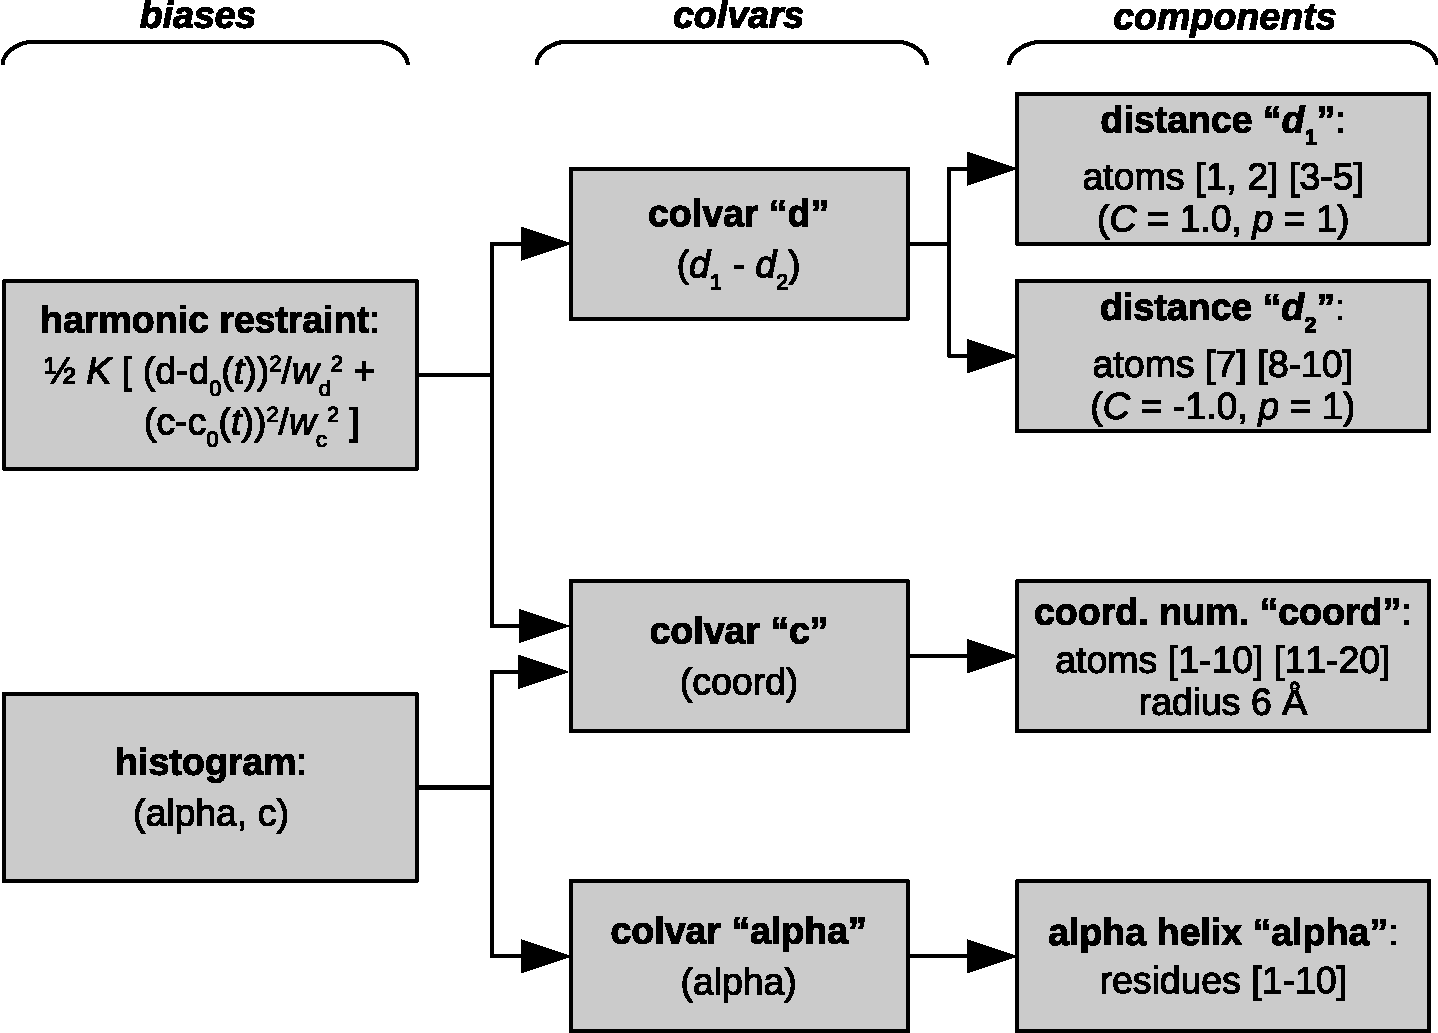
\includegraphics[width=12cm]{figures/colvars_diagram}}
\cvvmdugonly{\includegraphics[width=12cm]{pictures/colvars_diagram}}
\cvrefmanonly{\ifdefined\HCode{\HCode{<img class="diagram" src="colvars_diagram.png" alt="Colvars diagram">}}\else\includegraphics[width=12cm]{colvars_diagram}\fi}
  \caption[Graphical representation of a Colvars configuration.]{Graphical representation of a Colvars configuration\cvlammpsonly{ \textbf{(note:} \emph{currently, the $\alpha$-helical content colvar is unavailable in LAMMPS)}}.
    The colvar called ``$d$'' is defined as the difference between two distances: the first distance ($d_{1}$) is taken between the center of mass of atoms 1 and 2 and that of atoms 3 to 5, the second ($d_{2}$) between atom 7 and the center of mass of atoms 8 to 10.
The difference $d = d_{1} - d_{2}$ is obtained by multiplying the two by a coefficient $C = +1$ or $C = -1$, respectively.
The colvar called ``$c$'' is the coordination number calculated between atoms 1 to 10 and atoms 11 to 20.  A harmonic restraint is applied to both $d$ and $c$: to allow using the same force constant $K$, both $d$ and $c$ are scaled by their respective fluctuation widths $w_d$ and $w_c$.
\cvnamebasedonly{A third colvar ``alpha'' is defined as the $\alpha$-helical content of residues 1 to 10.}
The values of ``$c$''\cvnamebasedonly{ and ``alpha''} are also recorded throughout the simulation as a joint 2-dimensional histogram.
}
  \label{fig:colvars_diagram}
\end{figure}

{%
% verbatim can't appear within commands
\noindent\ttfamily
colvar \{\\
\-~~\# difference of two distances\\
\-~~name d \\
\-~~width 0.2  \# 0.2 \AA{} of estimated fluctuation width \\
\-~~distance \{\\
\-~~~~componentCoeff  1.0\\
\-~~~~group1 \{ atomNumbers 1 2 \}\\
\-~~~~group2 \{ atomNumbers 3 4 5 \}\\
\-~~\}\\
\-~~distance \{\\
\-~~~~componentCoeff -1.0\\
\-~~~~group1 \{ atomNumbers 7 \}\\
\-~~~~group2 \{ atomNumbers 8 9 10 \}\\
\-~~\}\\
\}\\
\\
colvar \{\\
\-~~name c\\
\-~~coordNum \{\\
\-~~~~cutoff 6.0\\
\-~~~~group1 \{ atomNumbersRange  1-10 \}\\
\-~~~~group2 \{ atomNumbersRange 11-20 \}\\
\-~~\}\\
\}\\}
\cvnamebasedonly{{%
\noindent\ttfamily\\
colvar \{\\
\-~~name alpha\\
\-~~alpha \{\\
\-~~~~psfSegID PROT\\
\-~~~~residueRange 1-10\\
\-~~\}\\
\}}}
{%
\noindent\ttfamily\\
\\
harmonic \{\\
\-~~colvars d c\\
\-~~centers 3.0 4.0\\
\-~~forceConstant 5.0\\
\}\\

\noindent histogram \{\\
\-~~colvars c\cvnamebasedonly{ alpha}\\
\}\\}

%\cvlammpsonly{\textbf{Note:} \emph{currently, the $\alpha$-helical content colvar is unavailable in LAMMPS, as it requires a name-based topology; future releases will overcome this limitation.}}

Section \ref{sec:colvar} explains how to define a colvar and its behavior, regardless of its specific functional form.
To define colvars that are appropriate to a specific physical system, Section \ref{sec:colvar_atom_groups} documents how to select atoms, and section \ref{sec:colvar} lists all of the available functional forms, which we call ``colvar components''.
Finally, section \ref{sec:colvarbias} lists the available methods and algorithms to perform biased simulations and multidimensional analysis of colvars.


\cvsubsec{Output files}{sec:colvars_output}

During a simulation with collective variables defined, the following three output files are written:

\begin{itemize}

\item A \emph{state file}, named \outputName\texttt{.colvars.state}; this file is in ASCII (plain text) format\cvnamdonly{, regardless of the value of \texttt{binaryOutput} in the NAMD configuration}.  This file is written at the end of the specified run\cvscriptonly{, but can also be written at any time with the command \texttt{cv save} (\ref{sec:cv_command_io})}.\\
  \emph{This is the only Colvars output file needed to continue a simulation.}

\item If the parameter \refkey{colvarsRestartFrequency}{Colvars-global|colvarsRestartFrequency} is larger than zero, a \emph{restart file} is written every that many steps: this file is fully equivalent to the final state file.
  The name of this file is \restartName\texttt{.colvars.state}.

\item If the parameter \refkey{colvarsTrajFrequency}{Colvars-global|colvarsTrajFrequency} is greater than 0 (default: 100), a \emph{trajectory file} is written during the simulation: its name is \outputName\texttt{.colvars.traj}; unlike the state file, it is not needed to restart a simulation, but can be used later for post-processing and analysis.

\end{itemize}

Other output files may also be written by specific methods, e.g.{} the ABF or metadynamics methods (\ref{sec:colvarbias_abf}, \ref{sec:colvarbias_meta}).
Like the trajectory file, they are needed only for analyzing, not continuing a simulation.
All such files' names also begin with the prefix \outputName.

\cvnamdonly{Lastly, the total energy of all biases or restraints applied to the colvars appears under the NAMD standard output, under the MISC column.}


\cvsec{Defining collective variables}{sec:colvar}

A collective variable is defined by the keyword \texttt{colvar} followed by its configuration options contained within curly braces:

{\bigskip\noindent\ttfamily
colvar \{\\
\-~~name xi\\
\-~~$<$other options$>$\\
\-~~function\_name \{\\
\-~~~~$<$parameters$>$\\
\-~~~~$<$atom selection$>$\\
\-~~\}\\
\}\\
}

\noindent{}There are multiple ways of defining a variable:
\begin{itemize}
\item The \emph{simplest and most common way} way is using one of the precompiled functions (here called ``components''), which are listed in section~\ref{sec:cvc_list}.  For example, using the keyword \texttt{rmsd} (section \ref{sec:cvc_rmsd}) defines the variable as the root mean squared deviation (RMSD) of the selected atoms.
\item A new variable may also be constructed as a linear or polynomial combination of the components listed in section~\ref{sec:cvc_list} (see \ref{sec:cvc_superp} for details).
\cvleptononly{
\item A user-defined mathematical function of the existing components (see list in section~\ref{sec:cvc_list}), or of the atomic coordinates directly (see the \texttt{cartesian} keyword in \ref{sec:cvc_cartesian}).
The function is defined through the keyword \refkey{customFunction}{colvar|customFunction} (see \ref{sec:colvar_custom_function} for details).
}
\cvscriptonly{
\item A user-defined Tcl function of the existing components (see list in section~\ref{sec:cvc_list}), or of the atomic coordinates directly (see the \texttt{cartesian} keyword in \ref{sec:cvc_cartesian}).
The function is provided by a separate Tcl script, and referenced through the keyword \refkey{scriptedFunction}{colvar|scriptedFunction} (see \ref{sec:colvar_scripted} for details).
}
\end{itemize}
Choosing a component (function) is the only parameter strictly required to define a collective variable.
It is also highly recommended to specify a name for the variable:
\begin{itemize}
\label{sec:colvar_general}
\item %
  \labelkey{colvar|name}
  \keydef
    {name}{%
    \texttt{colvar}}{%
    Name of this colvar}{%
    string}{%
    ``\texttt{colvar}'' + numeric id}{%
    The name is an unique case-sensitive string which allows the
    Colvars module to identify this colvar unambiguously; it is also
    used in the trajectory file to label to the columns corresponding
    to this colvar.}

\end{itemize}


\cvsubsec{Choosing a function}{sec:cvc_list}

In this context, the function that computes a colvar is called a \emph{component}.
A component's choice and definition consists of including in the variable's configuration a keyword indicating the type of function (e.g.{} \texttt{rmsd}), followed by a definition block specifying the atoms involved (see \ref{sec:colvar_atom_groups}) and any additional parameters (cutoffs, ``reference'' values, \ldots).
\emph{At least one component must be chosen to define a variable:} if none of the keywords listed below is found, an error is raised.

The following components implement functions with a scalar value (i.e.{} a real number):
\begin{itemize}
\item \refkey{distance}{colvar|distance}: distance between two groups;
\item \refkey{distanceZ}{colvar|distanceZ}: projection of a distance vector on an axis;
\item \refkey{distanceXY}{colvar|distanceXY}: projection of a distance vector on a plane;
\item \refkey{distanceInv}{colvar|distanceInv}: mean distance between two groups of atoms (e.g.~NOE-based distance);
\item \refkey{angle}{colvar|angle}: angle between three groups;
\item \refkey{dihedral}{colvar|dihedral}: torsional (dihedral) angle between four groups;
\item \refkey{dipoleAngle}{colvar|dipoleAngle}: angle between two groups and dipole of a third group;
\item \refkey{dipoleMagnitude}: magnitude of the dipole of a group of atoms;
\item \refkey{polarTheta}{colvar|polarTheta}: polar angle of a group in spherical coordinates;
\item \refkey{polarPhi}{colvar|polarPhi}: azimuthal angle of a group in spherical coordinates;
\item \refkey{coordNum}{colvar|coordNum}: coordination number between two groups;
\item \refkey{selfCoordNum}{colvar|selfCoordNum}: coordination number of atoms within a
  group;
\item \refkey{hBond}{colvar|hBond}: hydrogen bond between two atoms;
\item \refkey{rmsd}{colvar|rmsd}: root mean square deviation (RMSD) from a set of
  reference coordinates;
\item \refkey{eigenvector}{colvar|eigenvector}: projection of the atomic coordinates on a
  vector;
\item \refkey{orientationAngle}{colvar|orientationAngle}: angle of the best-fit rotation from
  a set of reference coordinates;
\item \refkey{orientationProj}{colvar|orientationProj}: cosine of \refkey{orientationProj}{colvar|orientationProj};
\item \refkey{spinAngle}{colvar|spinAngle}: projection orthogonal to an axis of the best-fit rotation
  from a set of reference coordinates;
\item \refkey{tilt}{colvar|tilt}: projection on an axis of the best-fit rotation
  from a set of reference coordinates;
\item \refkey{gyration}{colvar|gyration}: radius of gyration of a group of atoms;
\item \refkey{inertia}{colvar|inertia}: moment of inertia of a group of atoms;
\item \refkey{inertiaZ}{colvar|inertiaZ}: moment of inertia of a group of atoms around a chosen axis;
\cvnamebasedonly{
\item \refkey{alpha}{colvar|alpha}: $\alpha$-helix content of a protein segment.
\item \refkey{dihedralPC}{colvar|dihedralPC}: projection of protein backbone dihedrals onto a dihedral principal component.
}
\end{itemize}

Some components do not return scalar, but vector values:
\begin{itemize}
\item \refkey{distanceVec}{colvar|distanceVec}: distance vector between two groups (length: 3);
\item \refkey{distanceDir}{colvar|distanceDir}: unit vector parallel to distanceVec (length: 3);
\item \refkey{cartesian}{colvar|cartesian}: vector of atomic Cartesian coordinates (length: $N$ times the number of Cartesian components requested, X, Y or Z);
\item \refkey{distancePairs}{colvar|distancePairs}: vector of mutual distances (length: $N_{\mathrm{1}}\times{}N_{\mathrm{2}}$);
\item \refkey{orientation}{colvar|orientation}: best-fit rotation, expressed as a unit quaternion (length: 4).
\end{itemize}

The types of components used in a colvar (scalar or not) determine the
properties of that colvar, and particularly which biasing or analysis methods
can be applied.

\textbf{What if ``X'' is not listed?} If a function type is not available on this list, it may be possible to define it as a polynomial superposition of existing ones (see \ref{sec:cvc_superp})\cvleptononly{, a custom function (see \ref{sec:colvar_custom_function})}\cvscriptonly{, or a scripted function (see \ref{sec:colvar_scripted})}.

In the rest of this section, all available component types are listed, along with their physical units and the ranges of values, if limited.
Such limiting values can be used to define \refkey{lowerBoundary}{colvar|lowerBoundary} and \refkey{upperBoundary}{colvar|upperBoundary} in the parent colvar.

For each type of component, the available configurations keywords are listed:
when two components share certain keywords, the second component references to
the documentation of the first one that uses that keyword.
The very few keywords that are available for all types of components are listed in a separate section \ref{sec:cvc_common}.

\newenvironment{cvcoptions}%
  {\noindent\textbf{List of keywords} (see also \ref{sec:cvc_superp} for additional options):
  \begin{itemize}}
  {
  \end{itemize}
}

\cvsubsec{Distances}{sec:cvc_distances}


\cvsubsubsec{\texttt{distance}: center-of-mass distance between two groups.}{sec:cvc_distance}
\labelkey{colvar|distance}

The \texttt{distance \{...\}} block defines a distance component between the two atom groups, \texttt{group1} and \texttt{group2}.

\begin{cvcoptions}
\item %
  \labelkey{colvar|distance|group1}
  \key
    {group1}{%
    \texttt{distance}}{%
    First group of atoms}{%
    Block \texttt{group1 \{...\}}}{%
    First group of atoms.}

\item %
  \labelkey{colvar|distance|group2}
  \simkey{group2}{\texttt{distance}}{group1}

\item %
  \labelkey{colvar|distance|forceNoPBC}
  \keydef
    {forceNoPBC}{%
    \texttt{distance}}{%
    Calculate absolute rather than minimum-image distance?}{%
    boolean}{%
    \texttt{no}}{%
    By default, in calculations with periodic boundary conditions, the
    \texttt{distance} component returns the distance according to the
    minimum-image convention. If this parameter is set to \texttt{yes},
    PBC will be ignored and the distance between the coordinates as maintained
    internally will be used. This is only useful in a limited number of
    special cases, e.g. to describe the distance between remote points
    of a single macromolecule, which cannot be split across periodic cell
    boundaries, and for which the minimum-image distance might give the
    wrong result because of a relatively small periodic cell.}

\item %
  \labelkey{colvar|distance|oneSiteTotalForce}
  \keydef
    {oneSiteTotalForce}{%
    \texttt{angle}, \texttt{dipoleAngle}, \texttt{dihedral}}{%
    Measure total force on group 1 only?}{%
    boolean}{%
    \texttt{no}}{%
    If this is set to \texttt{yes}, the total force is measured along
    a vector field (see equation~(\ref{eq:gradient_vector}) in
    section~\ref{sec:colvarbias_abf}) that only involves atoms of
    \texttt{group1}.  This option is only useful for ABF, or custom
    biases that compute total forces.  See
    section~\ref{sec:colvarbias_abf} for details.}

\end{cvcoptions}

The value returned is a positive number (in \AA), ranging from $0$
to the largest possible interatomic distance within the chosen
boundary conditions (with PBCs, the minimum image convention is used
unless the \texttt{forceNoPBC} option is set).


\cvsubsubsec{\texttt{distanceZ}: projection of a distance vector on an axis.}{sec:cvc_distanceZ}
\labelkey{colvar|distanceZ}

The \texttt{distanceZ~\{...\}} block defines a distance projection
component, which can be seen as measuring the distance between two
groups projected onto an axis, or the position of a group along such
an axis.  The axis can be defined using either one reference group and
a constant vector, or dynamically based on two reference groups.
One of the groups can be set to a dummy atom to allow the use of an absolute Cartesian coordinate.

\begin{cvcoptions}
\item %
  \labelkey{colvar|distanceZ|main}
  \key
    {main}{%
    \texttt{distanceZ}}{%
    Main group of atoms}{%
    Block \texttt{main \{...\}}}{%
    Group of atoms whose position $\bm{r}$ is measured.}

\item %
  \labelkey{colvar|distanceZ|ref}
  \key
    {ref}{%
    \texttt{distanceZ}}{%
    Reference group of
    atoms}{%
    Block \texttt{ref \{...\}}}{%
    Reference group of atoms.  The position of its center of mass is
    noted $\bm{r}_1$ below.}

\item %
  \labelkey{colvar|distanceZ|ref2}
  \keydef
    {ref2}{%
    \texttt{distanceZ}}{%
    Secondary reference
    group}{%
    Block \texttt{ref2 \{...\}}}{%
    none}{%
    Optional group of reference atoms, whose position $\bm{r}_2$ can
    be used to define a dynamic projection axis: $\bm{e}=(\| \bm{r}_2
    - \bm{r}_1\|)^{-1} \times (\bm{r}_2 - \bm{r}_1)$.  In this case,
    the origin is $\bm{r}_m = 1/2 (\bm{r}_1+\bm{r}_2)$, and the value
    of the component is $\bm{e} \cdot (\bm{r}-\bm{r}_m)$.}

\item %
  \labelkey{colvar|distanceZ|axis}
  \keydef
    {axis}{%
    \texttt{distanceZ}}{%
    Projection axis (\AA{})}{%
    \texttt{(x, y, z)} triplet}{%
    \texttt{(0.0, 0.0, 1.0)}}{%
    The three components of this vector define a
    projection axis $\bm{e}$ for the distance vector $\bm{r} -
    \bm{r}_1$ joining the centers of groups \texttt{ref} and
    \texttt{main}. The value of the component is then $\bm{e} \cdot
    (\bm{r}-\bm{r}_1)$.  The vector should be written as three
    components separated by commas and enclosed in parentheses.}

\item %
  \dupkey{forceNoPBC}{\texttt{distanceZ}}{colvar|distance|forceNoPBC}{\texttt{distance} component}

\item %
  \dupkey{oneSiteTotalForce}{\texttt{distanceZ}}{colvar|distance|oneSiteTotalForce}{\texttt{distance} component}
\end{cvcoptions}
This component returns a number (in \AA{}) whose range is determined
by the chosen boundary conditions.  For instance, if the $z$ axis is
used in a simulation with periodic boundaries, the returned value ranges
between $-b_{z}/2$ and $b_{z}/2$, where $b_{z}$ is the box length
along $z$ (this behavior is disabled if \texttt{forceNoPBC} is set).


\cvsubsubsec{\texttt{distanceXY}: modulus of the projection of a distance vector on a plane.}{sec:cvc_distanceXY}
\labelkey{colvar|distanceXY}

The \texttt{distanceXY~\{...\}} block defines a distance projected on
a plane, and accepts the same keywords as the component \texttt{distanceZ}, i.e.
\texttt{main}, \texttt{ref}, either \texttt{ref2} or \texttt{axis},
and \texttt{oneSiteTotalForce}.  It returns the norm of the
projection of the distance vector between \texttt{main} and
\texttt{ref} onto the plane orthogonal to the axis.  The axis is
defined using the \texttt{axis} parameter or as the vector joining
\texttt{ref} and \texttt{ref2} (see \texttt{distanceZ} above).

\begin{cvcoptions}
\item %
  \dupkey{main}{\texttt{distanceXY}}{colvar|distanceZ|main}{\texttt{distanceZ} component}
\item %
  \dupkey{ref}{\texttt{distanceXY}}{colvar|distanceZ|ref}{\texttt{distanceZ} component}
\item %
  \dupkey{ref2}{\texttt{distanceXY}}{colvar|distanceZ|ref2}{\texttt{distanceZ} component}
\item %
  \dupkey{axis}{\texttt{distanceXY}}{colvar|distanceZ|axis}{\texttt{distanceZ} component}
\item %
  \dupkey{forceNoPBC}{\texttt{distanceXY}}{colvar|distance|forceNoPBC}{\texttt{distance} component}
\item %
  \dupkey{oneSiteTotalForce}{\texttt{distanceZ}}{colvar|distance|oneSiteTotalForce}{\texttt{distance} component}
\end{cvcoptions}



\cvsubsubsec{\texttt{distanceVec}: distance vector  between two groups.}{sec:cvc_distanceVec}
\labelkey{colvar|distanceVec}

The \texttt{distanceVec~\{...\}} block defines
a distance vector component, which accepts the same keywords as
the component \texttt{distance}: \texttt{group1}, \texttt{group2}, and
\texttt{forceNoPBC}. Its value is the 3-vector joining the centers
of mass of \texttt{group1} and \texttt{group2}.

\begin{cvcoptions}
\item %
  \dupkey{group1}{\texttt{distanceVec}}{colvar|distance|group1}{\texttt{distance} component}
\item %
  \simkey{group2}{\texttt{distanceVec}}{group1}
\item %
  \dupkey{forceNoPBC}{\texttt{distanceVec}}{colvar|distance|forceNoPBC}{\texttt{distance} component}
\item %
  \dupkey{oneSiteTotalForce}{\texttt{distanceVec}}{colvar|distance|oneSiteTotalForce}{\texttt{distance} component}
\end{cvcoptions}



\cvsubsubsec{\texttt{distanceDir}: distance unit vector between two groups.}{sec:cvc_distanceDir}
\labelkey{colvar|distanceDir}

The \texttt{distanceDir~\{...\}} block defines
a distance unit vector component, which accepts the same keywords as
the component \texttt{distance}: \texttt{group1}, \texttt{group2}, and
\texttt{forceNoPBC}.  It returns a
3-dimensional unit vector $\mathbf{d} = (d_{x}, d_{y}, d_{z})$, with
$|\mathbf{d}| = 1$.

\begin{cvcoptions}
\item %
  \dupkey{group1}{\texttt{distanceDir}}{colvar|distance|group1}{\texttt{distance} component}
\item %
  \simkey{group2}{\texttt{distanceDir}}{group1}
\item %
  \dupkey{forceNoPBC}{\texttt{distanceDir}}{colvar|distance|forceNoPBC}{\texttt{distance} component}
\item %
  \dupkey{oneSiteTotalForce}{\texttt{distanceDir}}{colvar|distance|oneSiteTotalForce}{\texttt{distance} component}
\end{cvcoptions}


\cvsubsubsec{\texttt{distanceInv}: mean distance between two groups of atoms.}{sec:cvc_distanceInv}
\labelkey{colvar|distanceInv}

The \texttt{distanceInv~\{...\}} block defines a generalized mean distance between two groups of atoms 1 and 2, weighted with exponent $1/n$:
\begin{equation}
  \label{eq:distanceInv}
  d_{\mathrm{1,2}}^{[n]} \; = \;   \left(\frac{1}{N_{\mathrm{1}}N_{\mathrm{2}}}\sum_{i,j} \left(\frac{1}{\Vert\mathbf{d}^{ij}\Vert}\right)^{n} \right)^{-1/n}
\end{equation}
where $\Vert\mathbf{d}^{ij}\Vert$ is the distance between atoms $i$ and $j$ in groups 1 and 2 respectively, and $n$ is an even integer.

\begin{cvcoptions}
\item %
  \dupkey{group1}{\texttt{distanceInv}}{colvar|distance|group1}{\texttt{distance} component}
\item %
  \simkey{group2}{\texttt{distanceInv}}{group1}
\item %
  \dupkey{oneSiteTotalForce}{\texttt{distanceInv}}{colvar|distance|oneSiteTotalForce}{\texttt{distance} component}
\item %
  \keydef
    {exponent}{%
    \texttt{distanceInv}}{%
    Exponent $n$ in equation~\ref{eq:distanceInv}}{%
    positive even integer}{%
    6}{Defines the exponent to which the individual distances are elevated before averaging.  The default value of 6 is useful for example to applying restraints based on NOE-measured distances.}
\end{cvcoptions}
This component returns a number in \AA{}, ranging from $0$ to the largest possible distance within the chosen boundary conditions.


\cvsubsec{Angles}{sec:cvc_angles}


\cvsubsubsec{\texttt{angle}: angle between three groups.}{sec:cvc_angle}
\labelkey{colvar|angle}

The \texttt{angle~\{...\}} block defines an angle, and contains the
three blocks \texttt{group1}, \texttt{group2} and \texttt{group3}, defining
the three groups.  It returns an angle (in degrees) within the
interval $[0:180]$.

\begin{cvcoptions}
\item %
  \dupkey{group1}{\texttt{angle}}{colvar|distance|group1}{\texttt{distance} component}
\item %
  \simkey{group2}{\texttt{angle}}{group1}
\item %
  \simkey{group3}{\texttt{angle}}{group1}
\item %
  \dupkey{forceNoPBC}{\texttt{angle}}{colvar|distance|forceNoPBC}{\texttt{distance} component}
\item %
  \dupkey{oneSiteTotalForce}{\texttt{angle}}{colvar|distance|oneSiteTotalForce}{\texttt{distance} component}
\end{cvcoptions}



\cvsubsubsec{\texttt{dipoleAngle}: angle between two groups and dipole of a third group.}{sec:cvc_dipoleAngle}
\labelkey{colvar|dipoleAngle}

The \texttt{dipoleAngle~\{...\}} block defines an angle, and contains the
three blocks \texttt{group1}, \texttt{group2} and \texttt{group3}, defining
the three groups, being \texttt{group1} the group where dipole is calculated. 
It returns an angle (in degrees) within the interval $[0:180]$.

\begin{cvcoptions}
\item %
  \dupkey{group1}{\texttt{dipoleAngle}}{colvar|distance|group1}{\texttt{distance} component}
\item %
  \simkey{group2}{\texttt{dipoleAngle}}{group1}
\item %
  \simkey{group3}{\texttt{dipoleAngle}}{group1}
\item %
  \dupkey{forceNoPBC}{\texttt{dipoleAngle}}{colvar|distance|forceNoPBC}{\texttt{distance} component}
\item %
  \dupkey{oneSiteTotalForce}{\texttt{dipoleAngle}}{colvar|distance|oneSiteTotalForce}{\texttt{distance} component}
\end{cvcoptions}


\cvsubsubsec{\texttt{dihedral}: torsional angle between four groups.}{sec:cvc_dihedral}
\labelkey{colvar|dihedral}

The \texttt{dihedral~\{...\}} block defines a torsional angle, and
contains the blocks \texttt{group1}, \texttt{group2}, \texttt{group3}
and \texttt{group4}, defining the four groups.  It returns an angle
(in degrees) within the interval $[-180:180]$.  The Colvars module
calculates all the distances between two angles taking into account
periodicity.  For instance, reference values for restraints or range
boundaries can be defined by using any real number of choice.

\begin{cvcoptions}
\item %
  \dupkey{group1}{\texttt{dihedral}}{colvar|distance|group1}{\texttt{distance} component}
\item %
  \simkey{group2}{\texttt{dihedral}}{group1}
\item %
  \simkey{group3}{\texttt{dihedral}}{group1}
\item %
  \simkey{group4}{\texttt{dihedral}}{group1}
\item %
  \dupkey{forceNoPBC}{\texttt{dihedral}}{colvar|distance|forceNoPBC}{\texttt{distance} component}
\item %
  \dupkey{oneSiteTotalForce}{\texttt{dihedral}}{colvar|distance|oneSiteTotalForce}{\texttt{distance} component}
\end{cvcoptions}


\cvsubsubsec{\texttt{polarTheta}: polar angle in spherical coordinates.}{sec:cvc_polarTheta}
\labelkey{colvar|polarTheta}

The \texttt{polarTheta~\{...\}} block defines the polar angle in
spherical coordinates, for the center of mass of a group of atoms 
described by the block \texttt{atoms}.  It returns an angle
(in degrees) within the interval $[0:180]$.
To obtain spherical coordinates in a frame of reference tied to
another group of atoms, use the \texttt{fittingGroup} (\ref{sec:colvar_atom_groups_ref_frame}) option
within the \texttt{atoms} block.
An example is provided in file \texttt{examples/11\_polar\_angles.in} of the Colvars public repository.

\begin{cvcoptions}
\item %
  \labelkey{colvar|polarTheta|atoms}
  \key
    {atoms}{%
    \texttt{polarPhi}}{%
    Atom group}{%
    \texttt{atoms~\{...\}} block}{%
    Defines the group of atoms for the COM of which the angle should be calculated.
    }
\end{cvcoptions}


\cvsubsubsec{\texttt{polarPhi}: azimuthal angle in spherical coordinates.}{sec:cvc_polarPhi}
\labelkey{colvar|polarPhi}

The \texttt{polarPhi~\{...\}} block defines the azimuthal angle in
spherical coordinates, for the center of mass of a group of atoms 
described by the block \texttt{atoms}. It returns an angle
(in degrees) within the interval $[-180:180]$.  The Colvars module
calculates all the distances between two angles taking into account
periodicity.  For instance, reference values for restraints or range
boundaries can be defined by using any real number of choice.
To obtain spherical coordinates in a frame of reference tied to
another group of atoms, use the \texttt{fittingGroup} (\ref{sec:colvar_atom_groups_ref_frame}) option
within the \texttt{atoms} block.
An example is provided in file \texttt{examples/11\_polar\_angles.in} of the Colvars public repository.


\begin{cvcoptions}
\item %
  \labelkey{colvar|polarPhi|atoms}
  \key
    {atoms}{%
    \texttt{polarPhi}}{%
    Atom group}{%
    \texttt{atoms~\{...\}} block}{%
    Defines the group of atoms for the COM of which the angle should be calculated.
    }
\end{cvcoptions}


\cvsubsec{Contacts}{sec:cvc_contacts}


\cvsubsubsec{\texttt{coordNum}: coordination number between two groups.}{sec:cvc_coordNum}
\labelkey{colvar|coordNum}

The \texttt{coordNum \{...\}} block defines
a coordination number (or number of contacts), which calculates the
function $(1-(d/d_0)^{n})/(1-(d/d_0)^{m})$, where $d_0$ is the
``cutoff'' distance, and $n$ and $m$ are exponents that can control
its long range behavior and stiffness \cite{Iannuzzi2003}.  This
function is summed over all pairs of atoms in \texttt{group1} and
\texttt{group2}:
\begin{equation}
  \label{eq:cvc_coordNum}
  C (\mathtt{group1}, \mathtt{group2}) \; = \; 
  \sum_{i\in\mathtt{group1}}\sum_{j\in\mathtt{group2}} {
    \frac{1 - (|\mathbf{x}_{i}-\mathbf{x}_{j}|/d_{0})^{n}}{
      1 - (|\mathbf{x}_{i}-\mathbf{x}_{j}|/d_{0})^{m} }
  }
\end{equation}

\begin{cvcoptions}

\item %
  \labelkey{colvar|coordNum|group1}
  \dupkey{group1}{\texttt{coordNum}}{colvar|distance|group1}{\texttt{distance} component}

\item %
  \labelkey{colvar|coordNum|group2}
  \simkey{group2}{\texttt{coordNum}}{group1}

\item %
  \labelkey{colvar|coordNum|cutoff}
  \keydef
    {cutoff}{%
    \texttt{coordNum}}{%
    ``Interaction'' distance (\AA)}{%
    positive decimal}{%
    4.0}{%
    This number defines the switching distance to define an
    interatomic contact: for $d \ll d_0$, the switching function
    $(1-(d/d_0)^{n})/(1-(d/d_0)^{m})$ is close to 1, at $d = d_0$ it
    has a value of $n/m$ ($1/2$ with the default $n$ and $m$), and at
    $d \gg d_0$ it goes to zero approximately like $d^{m-n}$.  Hence,
    for a proper behavior, $m$ must be larger than $n$.}

\item %
  \labelkey{colvar|coordNum|cutoff3}
  \keydef
    {cutoff3}{%
    \texttt{coordNum}}{%
    Reference distance vector (\AA)}{%
    ``\texttt{(x, y, z)}'' triplet of positive decimals}{%
    \texttt{(4.0, 4.0, 4.0)}}{%
    The three components of this vector define three different cutoffs
    $d_{0}$ for each direction.  This option is mutually exclusive with
    \texttt{cutoff}.}

\item %
  \labelkey{colvar|coordNum|expNumer}
  \keydef
    {expNumer}{%
    \texttt{coordNum}}{%
    Numerator exponent}{%
    positive even integer}{%
    6}{%
    This number defines the $n$ exponent for the switching function.}

\item %
  \labelkey{colvar|coordNum|expDenom}
  \keydef
    {expDenom}{%
    \texttt{coordNum}}{%
    Denominator exponent}{%
    positive even integer}{%
    12}{%
    This number defines the $m$ exponent for the switching function.}

\item %
  \labelkey{colvar|coordNum|group2CenterOnly}
  \keydef
    {group2CenterOnly}{%
    \texttt{coordNum}}{%
    Use only \texttt{group2}'s center of
    mass}{%
    boolean}{%
    \texttt{off}}{%
    If this option is \texttt{on}, only contacts between each atoms in \texttt{group1} and the center of mass of     \texttt{group2} are calculated (by default, the sum extends over all pairs of atoms in \texttt{group1} and \texttt{group2}).
If \texttt{group2} is a \texttt{dummyAtom}, this option is set to \texttt{yes} by default.
}

\item %
    \labelkey{colvar|coordNum|tolerance}
    \keydef
     {tolerance}{%
     \texttt{coordNum}}{%
     Pairlist control}{%
    decimal}{%
    0.0}{This controls the pairlist feature, dictating the minimum value for each summation element in Eq.~\ref{eq:cvc_coordNum} such that the pair that contributed the summation element is included in subsequent simulation timesteps until the next pairlist recalculation. For most applications, this value should be small (eg. 0.001) to avoid missing important contributions to the overall sum. Higher values will improve performance by reducing the number of pairs that contribute to the sum. Values above 1 will exclude all possible pair interactions. Similarly, values below 0 will never exclude a pair from consideration. To ensure continuous forces, Eq.~\ref{eq:cvc_coordNum} is further modified by subtracting the tolerance and then rescaling so that each pair covers the range $\left[0, 1\right]$.
  }

\item %
    \labelkey{colvar|coordNum|pairListFrequency}
    \keydef
     {pairListFrequency}{%
     \texttt{coordNum}}{%
     Pairlist regeneration frequency}{%
    positive integer}{%
    100}{This controls the pairlist feature, dictating how many steps are taken between regenerating pairlists if the tolerance is greater than 0.
  }
\end{cvcoptions}

This component returns a dimensionless number, which ranges from
approximately 0 (all interatomic distances are much larger than the
cutoff) to $N_{\mathtt{group1}} \times N_{\mathtt{group2}}$ (all distances
are less than the cutoff), or $N_{\mathtt{group1}}$ if
\texttt{group2CenterOnly} is used.  For performance reasons, at least
one of \texttt{group1} and \texttt{group2} should be of limited size or \texttt{group2CenterOnly} should be used: the cost of the loop over all pairs grows as $N_{\mathtt{group1}} \times N_{\mathtt{group2}}$.
Setting $\mathtt{tolerance} > 0$ ameliorates this to some degree, although every pair is still checked to regenerate the pairlist.



\cvsubsubsec{\texttt{selfCoordNum}: coordination number between atoms within a group.}{sec:cvc_selfCoordNum}
\labelkey{colvar|selfCoordNum}

The \texttt{selfCoordNum \{...\}} block defines
a coordination number similarly to the component \texttt{coordNum},
but the function is summed over atom pairs within \texttt{group1}:
\begin{equation}
  \label{eq:cvc_selfCoordNum}
  C (\mathtt{group1}) \; = \; 
  \sum_{i\in\mathtt{group1}}\sum_{j > i} {
    \frac{1 - (|\mathbf{x}_{i}-\mathbf{x}_{j}|/d_{0})^{n}}{
      1 - (|\mathbf{x}_{i}-\mathbf{x}_{j}|/d_{0})^{m} }
  }
\end{equation}
The keywords accepted by \texttt{selfCoordNum} are a subset of
those accepted by \texttt{coordNum}, namely \texttt{group1}
(here defining \emph{all} of the atoms to be considered),
\texttt{cutoff}, \texttt{expNumer}, and \texttt{expDenom}.

\begin{cvcoptions}
\item %
  \dupkey{group1}{\texttt{selfCoordNum}}{colvar|coordNum|group1}{\texttt{coordNum} component}
\item %
  \dupkey{cutoff}{\texttt{selfCoordNum}}{colvar|coordNum|cutoff}{\texttt{coordNum} component}
\item %
  \dupkey{cutoff3}{\texttt{selfCoordNum}}{colvar|coordNum|cutoff3}{\texttt{coordNum} component}
\item %
  \dupkey{expNumer}{\texttt{selfCoordNum}}{colvar|coordNum|expNumer}{\texttt{coordNum} component}
\item %
  \dupkey{expDenom}{\texttt{selfCoordNum}}{colvar|coordNum|expDenom}{\texttt{coordNum} component}
\item %
  \dupkey{tolerance}{\texttt{selfCoordNum}}{colvar|coordNum|tolerance}{\texttt{coordNum} component}
\item %
  \dupkey{pairListFrequency}{\texttt{selfCoordNum}}{colvar|coordNum|pairListFrequency}{\texttt{coordNum} component}
\end{cvcoptions}

This component returns a dimensionless number, which ranges from
approximately 0 (all interatomic distances much larger than the
cutoff) to $N_{\mathtt{group1}} \times (N_{\mathtt{group1}} - 1) / 2$ (all
distances within the cutoff).  For performance reasons,
\texttt{group1} should be of limited size, because the cost of the
loop over all pairs grows as $N_{\mathtt{group1}}^2$.



\cvsubsubsec{\texttt{hBond}: hydrogen bond between two atoms.}{sec:cvc_hBond}
\labelkey{colvar|hBond}

The \texttt{hBond \{...\}} block defines a hydrogen
bond, implemented as a coordination number (eq.~\ref{eq:cvc_coordNum})
between the donor and the acceptor atoms.  Therefore, it accepts the
same options \texttt{cutoff} (with a different default value of
3.3~\AA{}), \texttt{expNumer} (with a default value of 6) and
\texttt{expDenom} (with a default value of 8).  Unlike
\texttt{coordNum}, it requires two atom numbers, \texttt{acceptor} and
\texttt{donor}, to be defined.  It returns an adimensional number,
with values between 0 (acceptor and donor far outside the cutoff
distance) and 1 (acceptor and donor much closer than the cutoff).

\begin{cvcoptions}
\item %
  \key
    {acceptor}{%
    \texttt{hBond}}{%
    Number of the acceptor atom}{%
    positive integer}{%
    Number that uses the same convention as \texttt{atomNumbers}.}
\item %
  \simkey{donor}{\texttt{hBond}}{acceptor}
\item %
  \dupkey{cutoff}{\texttt{hBond}}{colvar|coordNum|cutoff}{\texttt{coordNum} component}\\
  \textbf{Note:} default value is 3.3~\AA.
\item %
  \dupkey{expNumer}{\texttt{hBond}}{colvar|coordNum|expNumer}{\texttt{coordNum} component}\\
  \textbf{Note:} default value is 6.
\item %
  \dupkey{expDenom}{\texttt{hBond}}{colvar|coordNum|expDenom}{\texttt{coordNum} component}\\
  \textbf{Note:} default value is 8.
\end{cvcoptions}


\cvsubsec{Collective metrics}{sec:cvc_collective}


\cvsubsubsec{\texttt{rmsd}: root mean square displacement (RMSD) from reference positions.}{sec:cvc_rmsd}
\labelkey{colvar|rmsd}

The block \texttt{rmsd~\{...\}} defines the root mean square replacement
(RMSD) of a group of atoms with respect to a reference structure.  For
each set of coordinates $\{ \mathbf{x}_1(t), \mathbf{x}_2(t), \ldots
\mathbf{x}_N(t) \}$, the colvar component \texttt{rmsd} calculates the
optimal rotation
$U^{\{\mathbf{x}_{i}(t)\}\rightarrow\{\mathbf{x}_{i}^{\mathrm{(ref)}}\}}$
that best superimposes the coordinates $\{\mathbf{x}_{i}(t)\}$ onto a
set of reference coordinates $\{\mathbf{x}_{i}^{\mathrm{(ref)}}\}$.
Both the current and the reference coordinates are centered on their
centers of geometry, $\mathbf{x}_{\mathrm{cog}}(t)$ and
$\mathbf{x}_{\mathrm{cog}}^{\mathrm{(ref)}}$.  The root mean square
displacement is then defined as:
\begin{equation}
  \label{eq:cvc_rmsd}
  { \mathrm{RMSD}(\{\mathbf{x}_{i}(t)\},
    \{\mathbf{x}_{i}^{\mathrm{(ref)}}\}) } \; = \; \sqrt{
    \frac{1}{N} \sum_{i=1}^{N} \left|
      U
      \left(\mathbf{x}_{i}(t) - \mathbf{x}_{\mathrm{cog}}(t)\right) -
      \left(\mathbf{x}_{i}^{\mathrm{(ref)}} -
        \mathbf{x}_{\mathrm{cog}}^{\mathrm{(ref)}} \right) \right|^{2} }
\end{equation}
The optimal rotation
$U^{\{\mathbf{x}_{i}(t)\}\rightarrow\{\mathbf{x}_{i}^{\mathrm{(ref)}}\}}$
is calculated within the formalism developed in
reference~\cite{Coutsias2004}, which guarantees a continuous
dependence of
$U^{\{\mathbf{x}_{i}(t)\}\rightarrow\{\mathbf{x}_{i}^{\mathrm{(ref)}}\}}$
with respect to $\{\mathbf{x}_{i}(t)\}$.

\begin{cvcoptions}

\item %
  \labelkey{colvar|rmsd|atoms}
  \key
    {atoms}{%
    \texttt{rmsd}}{%
    Atom group}{%
    \texttt{atoms~\{...\}} block}{%
    Defines the group of atoms of which the RMSD should be calculated.
    Optimal fit options (such as \texttt{refPositions} and
    \texttt{rotateReference}) should typically NOT be set within this
    block. Exceptions to this rule are the special cases discussed in
    the \emph{Advanced usage} paragraph below.
    }

\item %
  \labelkey{colvar|rmsd|refPositions}
  \key
    {refPositions}{%
    \texttt{rmsd}}{%
    Reference coordinates}{%
    space-separated list of \texttt{(x, y, z)} triplets}{%
    This option (mutually exclusive with \texttt{refPositionsFile}) sets the reference coordinates for RMSD calculation, and uses these to compute the roto-translational fit.  
    It is functionally equivalent to the option \refkey{refPositions}{atom-group|refPositions} in the atom group definition, which also supports more advanced fitting options.
    }

\item %
  \labelkey{colvar|rmsd|refPositionsFile}
  \key
    {refPositionsFile}{%
    \texttt{rmsd}}{%
    Reference coordinates file}{%
    UNIX filename}{%
    This option (mutually exclusive with \texttt{refPositions}) sets the reference coordinates for RMSD calculation, and uses these to compute the roto-translational fit.  
    It is functionally equivalent to the option \refkey{refPositionsFile}{atom-group|refPositionsFile} in the atom group definition, which also supports more advanced fitting options.
    }

\cvnamebasedonly{
\item %
  \labelkey{colvar|rmsd|refPositionsCol}
  \key
    {refPositionsCol}{%
    \texttt{rmsd}}{%
    PDB column containing atom flags}{%
    \texttt{O}, \texttt{B}, \texttt{X}, \texttt{Y}, or \texttt{Z}}{%
    If \texttt{refPositionsFile} is a PDB file that contains all the atoms in the topology, this option may be provided to set which PDB field is used to flag the reference coordinates for \texttt{atoms}.
  }

\item %
  \labelkey{colvar|rmsd|refPositionsColValue}
  \key
    {refPositionsColValue}{%
    \texttt{rmsd}}{%
    Atom selection flag in the PDB column}{%
    positive decimal}{%
    If defined, this value identifies in the PDB column
    \texttt{refPositionsCol} of the file \texttt{refPositionsFile}
    which atom positions are to be read.  Otherwise, all positions
    with a non-zero value are read.
  }
}
\end{cvcoptions}
This component returns a positive real number (in \AA).


\cvsubsubsec{Advanced usage of the \texttt{rmsd} component.}{sec:cvc_rmsd_advanced}
In the standard usage as described above, the \texttt{rmsd} component
calculates a minimum RMSD, that is, current coordinates are optimally
fitted onto the same reference coordinates that are used to 
compute the RMSD value. The fit itself is handled by the atom group
object, whose parameters are automatically set by the \texttt{rmsd}
component.
For very specific applications, however, it may be
useful to control the fitting process separately from the definition
of the reference coordinates, to evaluate various types of
non-minimal RMSD values. This can be achieved by setting the
related options (\texttt{refPositions}, etc.) explicitly in the
atom group block. This allows for the following non-standard cases:

\begin{enumerate}
\item applying the optimal translation, but no rotation
(\texttt{rotateReference off}), to bias or restrain the shape and
orientation, but not the position of the atom group;
\item applying the optimal rotation, but no translation
(\texttt{centerReference off}), to bias or restrain the shape and
position, but not the orientation of the atom group;
\item disabling the application of optimal roto-translations, which
lets the RMSD component decribe the deviation of atoms
from fixed positions in the laboratory frame: this allows for custom
positional restraints within the Colvars module;
\item fitting the atomic positions to different reference coordinates
than those used in the RMSD calculation itself;
\item applying the optimal rotation and/or translation from a separate
atom group, defined through \texttt{fittingGroup}: the RMSD then
reflects the deviation from reference coordinates in a separate, moving
reference frame.
\end{enumerate}


\cvscriptonly{
\cvsubsubsec{Path collective variables}{sec:pathcv}

An application of the \texttt{rmsd} component is "path collective variables",\cite{Branduardi2007}
which are implemented as Tcl-scripted combinations or RMSDs.
The implementation is available as file \texttt{colvartools/pathCV.tcl}, and
an example is provided in file \texttt{examples/10\_pathCV.namd} of the Colvars public repository.}


\cvsubsubsec{\texttt{eigenvector}: projection of the atomic  coordinates on a vector.}{sec:cvc_eigenvector}
\labelkey{colvar|eigenvector}

The block \texttt{eigenvector~\{...\}} defines the projection of the coordinates
of a group of atoms (or more precisely, their deviations from the
reference coordinates) onto a vector in $\mathbb{R}^{3n}$, where $n$ is the
number of atoms in the group. The computed quantity is the
total projection:
\begin{equation}
  \label{eq:cvc_eigenvector}
  { p(\{\mathbf{x}_{i}(t)\},
    \{\mathbf{x}_{i}^{\mathrm{(ref)}}\}) } \; = \; {
    \sum_{i=1}^{n}  \mathbf{v}_{i} \cdot
    \left(U(\mathbf{x}_{i}(t) - \mathbf{x}_{\mathrm{cog}}(t)) -
      (\mathbf{x}_{i}^{\mathrm{(ref)}} -
      \mathbf{x}_{\mathrm{cog}}^{\mathrm{(ref)}}) \right)\mathrm{,} }
\end{equation}
where, as in the \texttt{rmsd} component, $U$ is the optimal rotation
matrix, $\mathbf{x}_{\mathrm{cog}}(t)$ and
$\mathbf{x}_{\mathrm{cog}}^{\mathrm{(ref)}}$ are the centers of
geometry of the current and reference positions respectively, and
$\mathbf{v}_{i}$ are the components of the vector for each atom.
Example choices for $(\mathbf{v}_{i})$ are an eigenvector
of the covariance matrix (essential mode), or a normal
mode of the system.  It is assumed that $\sum_{i}\mathbf{v}_{i} = 0$:
otherwise, the Colvars module centers the $\mathbf{v}_{i}$
automatically when reading them from the configuration.

\begin{cvcoptions}
\item %
  \dupkey{atoms}{\texttt{eigenvector}}{colvar|rmsd|atoms}{\texttt{rmsd} component}
\item %
  \dupkey{refPositions}{\texttt{eigenvector}}{colvar|rmsd|refPositions}{\texttt{rmsd} component}
\item %
  \dupkey{refPositionsFile}{\texttt{eigenvector}}{colvar|rmsd|refPositionsFile}{\texttt{rmsd} component}
\cvnamebasedonly{
\item %
  \dupkey{refPositionsCol}{\texttt{eigenvector}}{colvar|rmsd|refPositionsCol}{\texttt{rmsd} component}
\item %
  \dupkey{refPositionsColValue}{\texttt{eigenvector}}{colvar|rmsd|refPositionsColValue}{\texttt{rmsd} component}
}

\item %
  \key
    {vector}{%
    \texttt{eigenvector}}{%
    Vector components}{%
    space-separated list of \texttt{(x, y, z)} triplets}{%
    This option (mutually exclusive with \texttt{vectorFile}) sets the values of the vector components.}

\item %
  \key
    {vectorFile}{%
    \texttt{eigenvector}}{%
    file containing vector components}{%
    UNIX filename}{%
    This option (mutually exclusive with \texttt{vector}) sets the name of a coordinate file containing the vector components; the file is read according to the same format used for \texttt{refPositionsFile}.
    \cvnamebasedonly{For a PDB file specifically, the components are read from the X, Y and Z fields.
      \textbf{Note:} \emph{The PDB file has limited precision and fixed-point numbers: in some cases, the vector components may not be accurately represented; a XYZ file should be used instead, containing floating-point numbers.}}
  }

\cvnamebasedonly{
\item %
  \key
    {vectorCol}{%
    \texttt{eigenvector}}{%
    PDB column used to flag participating atoms}{%
    \texttt{O} or \texttt{B}}{%
    Analogous to \texttt{atomsCol}.}

\item %
  \key
    {vectorColValue}{%
    \texttt{eigenvector}}{%
    Value used to flag participating atoms in the PDB file}{%
    positive decimal}{%
    Analogous to \texttt{atomsColValue}.}
}

\item %
  \keydef
    {differenceVector}{%
    \texttt{eigenvector}}{%
    The $3n$-dimensional vector is the difference between \texttt{vector} and \texttt{refPositions}}{%
    boolean}{%
    \texttt{off}}{%
    If this option is \texttt{on}, the numbers provided by \texttt{vector}\cvnamebasedonly{ or \texttt{vectorFile}} are interpreted as another set of positions, $\mathbf{x}_{i}'$: the vector $\mathbf{v}_{i}$ is then defined as $\mathbf{v}_{i} = \left(\mathbf{x}_{i}' - \mathbf{x}_{i}^{\mathrm{(ref)}}\right)$.
This allows to conveniently define a colvar $\xi$ as a projection on the linear transformation between two sets of positions, ``A'' and ``B''.
For convenience, the vector is also normalized so that $\xi = 0$ when the atoms are at the set of positions ``A'' and $\xi = 1$ at the set of positions ``B''.
}
\end{cvcoptions}
This component returns a number (in \AA), whose value ranges between
the smallest and largest absolute positions in the unit cell during
the simulations (see also \texttt{distanceZ}).  Due to the
normalization in eq.~\ref{eq:cvc_eigenvector}, this range does not
depend on the number of atoms involved.


\cvsubsubsec{\texttt{gyration}: radius of gyration of a group  of atoms.}{sec:cvc_gyration}
\labelkey{colvar|gyration}

The block \texttt{gyration~\{...\}} defines the
parameters for calculating the radius of gyration of a group of atomic
positions $\{ \mathbf{x}_1(t), \mathbf{x}_2(t), \ldots \mathbf{x}_N(t)
\}$ with respect to their center of geometry,
$\mathbf{x}_{\mathrm{cog}}(t)$:
\begin{equation}
  \label{eq:colvar_gyration}
  R_{\mathrm{gyr}} \; = \; \sqrt{ \frac{1}{N}
    \sum_{i=1}^{N} \left|\mathbf{x}_{i}(t) -
      \mathbf{x}_{\mathrm{cog}}(t)\right|^{2} }
\end{equation}
This component must contain one \texttt{atoms~\{...\}} block to
define the atom group, and returns a positive number, expressed in
\AA{}.

\begin{cvcoptions}
\item %
  \dupkey{atoms}{\texttt{gyration}}{colvar|rmsd|atoms}{\texttt{rmsd} component}
\end{cvcoptions}


\cvsubsubsec{\texttt{inertia}: total moment of inertia of a group  of atoms.}{sec:cvc_inertia}
\labelkey{colvar|inertia}

The block \texttt{inertia~\{...\}} defines the
parameters for calculating the total moment of inertia of a group of atomic
positions $\{ \mathbf{x}_1(t), \mathbf{x}_2(t), \ldots \mathbf{x}_N(t)
\}$ with respect to their center of geometry,
$\mathbf{x}_{\mathrm{cog}}(t)$:
\begin{equation}
  \label{eq:colvar_inertia}
  I \; = \; \sum_{i=1}^{N} \left|\mathbf{x}_{i}(t) -
      \mathbf{x}_{\mathrm{cog}}(t)\right|^{2}
\end{equation}
\emph{Note that all atomic masses are set to 1 for simplicity.}
This component must contain one \texttt{atoms~\{...\}} block to
define the atom group, and returns a positive number, expressed in
\AA{}$^{2}$.

\begin{cvcoptions}
\item %
  \dupkey{atoms}{\texttt{inertia}}{colvar|rmsd|atoms}{\texttt{rmsd} component}
\end{cvcoptions}


\cvsubsubsec{\texttt{dipoleMagnitude}: dipole magnitude of a group of atoms.}{sec:cvc_dipoleMagnitude}
The \texttt{dipoleMagnitude~\{...\}} block defines the dipole magnitude of a group of atoms (norm of the dipole moment's vector), being \texttt{atoms} the group where dipole magnitude is calculated.
It returns the magnitude in elementary charge $e$ times \cvnamdonly{\AA}\cvvmdonly{\AA}\cvlammpsonly{(length unit)}.

\begin{cvcoptions}
\item %
  \dupkey{atoms}{\texttt{dipoleMagnitude}}{colvar|rmsd|atoms}{\texttt{rmsd} component}
\end{cvcoptions}


\cvsubsubsec{\texttt{inertiaZ}: total moment of inertia of a group of atoms around a chosen axis.}{sec:cvc_inertiaZ}
\labelkey{colvar|inertiaZ}

The block \texttt{inertiaZ~\{...\}} defines the
parameters for calculating the component along the axis $\mathbf{e}$ of the moment of inertia of a group of atomic
positions $\{ \mathbf{x}_1(t), \mathbf{x}_2(t), \ldots \mathbf{x}_N(t)
\}$ with respect to their center of geometry,
$\mathbf{x}_{\mathrm{cog}}(t)$:
\begin{equation}
  \label{eq:colvar_inertia_z}
  I_{\mathbf{e}} \; = \; \sum_{i=1}^{N} \left(\left(\mathbf{x}_{i}(t) -
      \mathbf{x}_{\mathrm{cog}}(t)\right)\cdot\mathbf{e}\right)^{2}
\end{equation}
\emph{Note that all atomic masses are set to 1 for simplicity.}
This component must contain one \texttt{atoms~\{...\}} block to
define the atom group, and returns a positive number, expressed in
\AA{}$^{2}$.


\begin{cvcoptions}
\item %
  \dupkey{atoms}{\texttt{inertiaZ}}{colvar|rmsd|atoms}{\texttt{rmsd} component}
\item %
  \keydef
    {axis}{%
    \texttt{inertiaZ}}{%
    Projection axis (\AA{})}{%
    \texttt{(x, y, z)} triplet}{%
    \texttt{(0.0, 0.0, 1.0)}}{%
    The three components of this vector define (when normalized) the
    projection axis $\mathbf{e}$.}
\end{cvcoptions}


\cvsubsec{Rotations}{sec:cvc_rotations}


\cvsubsubsec{\texttt{orientation}: orientation from reference coordinates.}{sec:cvc_orientation}
\labelkey{colvar|orientation}

The block \texttt{orientation~\{...\}} returns the
same optimal rotation used in the \texttt{rmsd} component to
superimpose the coordinates $\{\mathbf{x}_{i}(t)\}$ onto a set of
reference coordinates $\{\mathbf{x}_{i}^{\mathrm{(ref)}}\}$.  Such
component returns a four dimensional vector $\mathsf{q} = (q_0, q_1,
q_2, q_3)$, with $\sum_{i} q_{i}^{2} = 1$; this \emph{quaternion}
expresses the optimal rotation $\{\mathbf{x}_{i}(t)\} \rightarrow
\{\mathbf{x}_{i}^{\mathrm{(ref)}}\}$ according to the formalism in
reference~\cite{Coutsias2004}.  The quaternion $(q_0, q_1, q_2, q_3)$
can also be written as $\left(\cos(\theta/2), \,
  \sin(\theta/2)\mathbf{u}\right)$, where $\theta$ is the angle and
$\mathbf{u}$ the normalized axis of rotation; for example, a rotation
of 90$^{\circ}$ around the $z$ axis is expressed as
``\texttt{(0.707, 0.0, 0.0, 0.707)}''.  The script
\texttt{quaternion2rmatrix.tcl} provides Tcl functions for converting
to and from a $4\times{}4$ rotation matrix in a format suitable for
usage in VMD.

As for the component \texttt{rmsd}, the available options are \texttt{atoms}, \texttt{refPositionsFile}\cvnamebasedonly{, \texttt{refPositionsCol} and \texttt{refPositionsColValue}, } and \texttt{refPositions}.

\textbf{Note:} \texttt{refPositions}and \texttt{refPositionsFile} define the set of positions \emph{from which} the optimal rotation is calculated, but this rotation is not applied to the coordinates of the atoms involved: it is used instead to define the variable itself.

\begin{cvcoptions}
\item %
  \dupkey{atoms}{\texttt{orientation}}{colvar|rmsd|atoms}{\texttt{rmsd} component}
\item %
  \dupkey{refPositions}{\texttt{orientation}}{colvar|rmsd|refPositions}{\texttt{rmsd} component}
\item %
  \dupkey{refPositionsFile}{\texttt{orientation}}{colvar|rmsd|refPositionsFile}{\texttt{rmsd} component}

\cvnamebasedonly{
\item %
  \dupkey{refPositionsCol}{\texttt{orientation}}{colvar|rmsd|refPositionsCol}{\texttt{rmsd} component}
\item %
  \dupkey{refPositionsColValue}{\texttt{orientation}}{colvar|rmsd|refPositionsColValue}{\texttt{rmsd} component}
}

\item %
  \keydef
    {closestToQuaternion}{%
    \texttt{orientation}}{%
    Reference rotation}{%
    ``\texttt{(q0, q1, q2, q3)}'' quadruplet}{%
    \texttt{(1.0, 0.0, 0.0, 0.0)} (``null'' rotation)}{%
    Between the two equivalent quaternions $(q_0, q_1, q_2, q_3)$ and
    $(-q_0, -q_1, -q_2, -q_3)$, the closer to \texttt{(1.0, 0.0, 0.0,
      0.0)} is chosen.  This simplifies the visualization of the
    colvar trajectory when sampled values are a smaller subset of all
    possible rotations.  \textbf{Note:} \emph {this only affects the
      output, never the dynamics}.}

\end{cvcoptions}

\textbf{Tip: stopping the rotation of a protein.}  To stop the
rotation of an elongated macromolecule in solution (and use an
anisotropic box to save water molecules), it is possible to define a
colvar with an \texttt{orientation} component, and restrain it throuh
the \texttt{harmonic} bias around the identity rotation, \texttt{(1.0,
  0.0, 0.0, 0.0)}.  Only the overall orientation of the macromolecule
is affected, and \emph{not} its internal degrees of freedom.  The user
should also take care that the macromolecule is composed by a single
chain, or disable \texttt{wrapAll} otherwise.



\cvsubsubsec{\texttt{orientationAngle}: angle of rotation from reference coordinates.}{sec:cvc_orientationAngle}
\labelkey{colvar|orientationAngle}

The block \texttt{orientationAngle~\{...\}} accepts the same base options as
the component \texttt{orientation}: \texttt{atoms}, \texttt{refPositions}, \texttt{refPositionsFile}\cvnamebasedonly{, \texttt{refPositionsCol} and \texttt{refPositionsColValue}}.
The returned value is the angle of rotation $\theta$ between the current and the reference positions.
This angle is expressed in degrees within the range [0$^{\circ}$:180$^{\circ}$].

\begin{cvcoptions}
\item %
  \dupkey{atoms}{\texttt{orientationAngle}}{colvar|rmsd|atoms}{\texttt{rmsd} component}
\item %
  \dupkey{refPositions}{\texttt{orientationAngle}}{colvar|rmsd|refPositions}{\texttt{rmsd} component}
\item %
  \dupkey{refPositionsFile}{\texttt{orientationAngle}}{colvar|rmsd|refPositionsFile}{\texttt{rmsd} component}

\cvnamebasedonly{
\item %
  \dupkey{refPositionsCol}{\texttt{orientationAngle}}{colvar|rmsd|refPositionsCol}{\texttt{rmsd} component}
\item %
  \dupkey{refPositionsColValue}{\texttt{orientationAngle}}{colvar|rmsd|refPositionsColValue}{\texttt{rmsd} component}
}
\end{cvcoptions}


\cvsubsubsec{\texttt{orientationProj}: cosine of the angle of rotation from reference coordinates.}  {sec:cvc_orientationProj}
\labelkey{colvar|orientationProj}

The block \texttt{orientationProj~\{...\}} accepts the same base options as
the component \texttt{orientation}: \texttt{atoms}, \texttt{refPositions}, \texttt{refPositionsFile}\cvnamebasedonly{, \texttt{refPositionsCol} and \texttt{refPositionsColValue}}.
The returned value is the cosine of the angle of rotation $\theta$ between the current and the reference positions.
The range of values is [-1:1].

\begin{cvcoptions}
\item %
  \dupkey{atoms}{\texttt{orientationProj}}{colvar|rmsd|atoms}{\texttt{rmsd} component}
\item %
  \dupkey{refPositions}{\texttt{orientationProj}}{colvar|rmsd|refPositions}{\texttt{rmsd} component}
\item %
  \dupkey{refPositionsFile}{\texttt{orientationProj}}{colvar|rmsd|refPositionsFile}{\texttt{rmsd} component}
\cvnamebasedonly{
\item %
  \dupkey{refPositionsCol}{\texttt{orientationProj}}{colvar|rmsd|refPositionsCol}{\texttt{rmsd} component}
\item %
  \dupkey{refPositionsColValue}{\texttt{orientationProj}}{colvar|rmsd|refPositionsColValue}{\texttt{rmsd} component}
}
\end{cvcoptions}


\cvsubsubsec{\texttt{spinAngle}: angle of rotation around a given axis.}{sec:cvc_spinAngle}
\labelkey{colvar|spinAngle}

The complete rotation described by \texttt{orientation} can optionally be decomposed into two sub-rotations: one is a ``\emph{spin}'' rotation around \textbf{e}, and the other a ``\emph{tilt}'' rotation around an axis orthogonal to \textbf{e}.
The component \texttt{spinAngle} measures the angle of the ``spin'' sub-rotation around \textbf{e}.

\begin{cvcoptions}
\item %
  \dupkey{atoms}{\texttt{spinAngle}}{colvar|rmsd|atoms}{\texttt{rmsd} component}
\item %
  \dupkey{refPositions}{\texttt{spinAngle}}{colvar|rmsd|refPositions}{\texttt{rmsd} component}
\item %
  \dupkey{refPositionsFile}{\texttt{spinAngle}}{colvar|rmsd|refPositionsFile}{\texttt{rmsd} component}
\cvnamebasedonly{
\item %
  \dupkey{refPositionsCol}{\texttt{spinAngle}}{colvar|rmsd|refPositionsCol}{\texttt{rmsd} component}
\item %
  \dupkey{refPositionsColValue}{\texttt{spinAngle}}{colvar|rmsd|refPositionsColValue}{\texttt{rmsd} component}
}
\item %
  \labelkey{colvar|spinAngle|axis}
  \keydef
    {axis}{%
    \texttt{tilt}}{%
    Special rotation axis (\AA{})}{%
    \texttt{(x, y, z)} triplet}{%
    \texttt{(0.0, 0.0, 1.0)}}{%
    The three components of this vector define (when normalized) the special rotation axis used to calculate the \texttt{tilt} and \texttt{spinAngle} components.}
\end{cvcoptions}
The component \texttt{spinAngle} returns an angle (in degrees) within the periodic interval $[-180:180]$.  

\textbf{Note:} the value of \texttt{spinAngle} is a continuous function almost everywhere, with the exception of configurations with the corresponding ``tilt'' angle equal to 180$^\circ$ (i.e.~the \texttt{tilt} component is equal to $-1$): in those cases, \texttt{spinAngle} is undefined.  If such configurations are expected, consider defining a \texttt{tilt} colvar using the same axis \textbf{e}, and restraining it with a lower wall away from $-1$.


\cvsubsubsec{\texttt{tilt}: cosine of the rotation orthogonal to a given axis.}{sec:cvc_tilt}
\labelkey{colvar|tilt}

The component \texttt{tilt} measures the cosine of the angle of the ``tilt'' sub-rotation, which combined with the ``spin'' sub-rotation provides the complete rotation of a group of atoms.
The cosine of the tilt angle rather than the tilt angle itself is implemented, because the latter is unevenly distributed even for an isotropic system: consider as an analogy the angle $\theta$ in the spherical coordinate system.
The component \texttt{tilt} relies on the same options as \texttt{spinAngle}, including the definition of the axis \textbf{e}.
The values of \texttt{tilt} are real numbers in the interval $[-1:1]$: the value $1$ represents an orientation fully parallel to \textbf{e} (tilt angle = 0$^\circ$), and the value $-1$ represents an anti-parallel orientation.

\begin{cvcoptions}
\item %
  \dupkey{atoms}{\texttt{tilt}}{colvar|rmsd|atoms}{\texttt{rmsd} component}
\item %
  \dupkey{refPositions}{\texttt{tilt}}{colvar|rmsd|refPositions}{\texttt{rmsd} component}
\item %
  \dupkey{refPositionsFile}{\texttt{tilt}}{colvar|rmsd|refPositionsFile}{\texttt{rmsd} component}
\cvnamebasedonly{
\item %
  \dupkey{refPositionsCol}{\texttt{tilt}}{colvar|rmsd|refPositionsCol}{\texttt{rmsd} component}
\item %
  \dupkey{refPositionsColValue}{\texttt{tilt}}{colvar|rmsd|refPositionsColValue}{\texttt{rmsd} component}
}
\item %
  \dupkey{axis}{\texttt{tilt}}{colvar|spinAngle|axis}{\texttt{spinAngle} component}
\end{cvcoptions}
 

\cvnamebasedonly{

\cvsubsec{Protein structure descriptors}{sec:cvc_protein}

\cvsubsubsec{\texttt{alpha}: $\alpha$-helix content of a protein segment.}{sec:cvc_alpha}
\labelkey{colvar|alpha}

The block \texttt{alpha~\{...\}} defines the
parameters to calculate the helical content of a segment of protein
residues.  The $\alpha$-helical content across the $N+1$ residues
$N_{0}$ to $N_{0}+N$ is calculated by the formula:
\begin{eqnarray}
  \label{eq:colvars_alpha}
  { 
    \alpha\left(
      \mathrm{C}_{\alpha}^{(N_{0})},
      \mathrm{O}^{(N_{0})},
      \mathrm{C}_{\alpha}^{(N_{0}+1)},
      \mathrm{O}^{(N_{0}+1)},
      \ldots
      \mathrm{N}^{(N_{0}+5)},
      \mathrm{C}_{\alpha}^{(N_{0}+5)},
      \mathrm{O}^{(N_{0}+5)},
      \ldots
      \mathrm{N}^{(N_{0}+N)},
      \mathrm{C}_{\alpha}^{(N_{0}+N)}
    \right)
  } \; = \; \; \; \; \\ \; \; \; \; {
    \nonumber
    \frac{1}{2(N-2)} 
    \sum_{n=N_{0}}^{N_{0}+N-2}
    \mathrm{angf}\left(
        \mathrm{C}_{\alpha}^{(n)},
        \mathrm{C}_{\alpha}^{(n+1)},
        \mathrm{C}_{\alpha}^{(n+2)}\right)
  } \; + \; {
    \frac{1}{2(N-4)} 
    \sum_{n=N_{0}}^{N_{0}+N-4}
    \mathrm{hbf}\left(
      \mathrm{O}^{(n)},
      \mathrm{N}^{(n+4)}\right) \mathrm{,}
  } \\
\end{eqnarray}
where the score function for the $\mathrm{C}_{\alpha} -
\mathrm{C}_{\alpha} - \mathrm{C}_{\alpha}$ angle is defined as: 
\begin{equation}
  \label{eq:colvars_alpha_Calpha}
  {
    \mathrm{angf}\left(
      \mathrm{C}_{\alpha}^{(n)},
      \mathrm{C}_{\alpha}^{(n+1)},
      \mathrm{C}_{\alpha}^{(n+2)}\right)
  } \; = \; {
    \frac{1 - \left(\theta(
        \mathrm{C}_{\alpha}^{(n)},
        \mathrm{C}_{\alpha}^{(n+1)},
        \mathrm{C}_{\alpha}^{(n+2)}) -
        \theta_{0}\right)^{2} /
      \left(\Delta\theta_{\mathrm{tol}}\right)^{2}}{
      1 - \left(\theta(
        \mathrm{C}_{\alpha}^{(n)},
        \mathrm{C}_{\alpha}^{(n+1)},
        \mathrm{C}_{\alpha}^{(n+2)}) -
        \theta_{0}\right)^{4} /
      \left(\Delta\theta_{\mathrm{tol}}\right)^{4}} \mathrm{,}
  }
\end{equation}
and the score function for the $\mathrm{O}^{(n)} \leftrightarrow
\mathrm{N}^{(n+4)}$ hydrogen bond is defined through a \texttt{hBond}
colvar component on the same atoms.

\begin{cvcoptions}

\item %
  \labelkey{colvar|alpha|residueRange}
  \key
    {residueRange}{%
      \texttt{alpha}}{%
      Potential $\alpha$-helical residues}{%
    ``$<$Initial residue number$>$-$<$Final residue number$>$''}{%
    This option specifies the range of residues on which this
    component should be defined.  The Colvars module looks for the
    atoms within these residues named ``\texttt{CA}'', ``\texttt{N}''
    and ``\texttt{O}'', and raises an error if any of those atoms is
    not found.}

\item %
  \labelkey{colvar|alpha|psfSegID}
  \key
    {psfSegID}{%
    \texttt{alpha}}{%
    PSF segment identifier}{%
    string (max 4 characters)}{%
    This option sets the PSF segment identifier for the residues
    specified in \texttt{residueRange}.  This option is only required
    when PSF topologies are used.}


\item %
  \labelkey{colvar|alpha|hBondCoeff}
  \keydef
    {hBondCoeff}{%
    \texttt{alpha}}{%
    Coefficient for the hydrogen bond term}{%
    positive between 0 and 1}{%
    0.5}{%
    This number specifies the contribution to the total value from the
    hydrogen bond terms.  0 disables the hydrogen bond terms, 1
    disables the angle terms.}

\item %
  \labelkey{colvar|alpha|angleRef}
  \keydef
    {angleRef}{%
    \texttt{alpha}}{%
    Reference $\mathrm{C}_{\alpha} -
    \mathrm{C}_{\alpha} - \mathrm{C}_{\alpha}$ angle}{%
    positive decimal}{%
    88$^{\circ}$}{%
    This option sets the reference angle used in the score function
    (\ref{eq:colvars_alpha_Calpha}).}

\item %
  \labelkey{colvar|alpha|angleTol}
  \keydef
    {angleTol}{%
    \texttt{alpha}}{%
    Tolerance in the $\mathrm{C}_{\alpha} -
    \mathrm{C}_{\alpha} - \mathrm{C}_{\alpha}$ angle}{%
    positive decimal}{%
    15$^{\circ}$}{%
    This option sets the angle tolerance used in the score function
    (\ref{eq:colvars_alpha_Calpha}).}

\item %
  \labelkey{colvar|alpha|hBondCutoff}
  \keydef
    {hBondCutoff}{%
    \texttt{alpha}}{%
    Hydrogen bond cutoff}{%
    positive decimal}{%
    3.3~\AA{}}{%
    Equivalent to the \texttt{cutoff} option in the \texttt{hBond}
    component.}

\item %
  \labelkey{colvar|alpha|hBondExpNumer}
  \keydef
    {hBondExpNumer}{%
    \texttt{alpha}}{%
    Hydrogen bond numerator exponent}{%
    positive integer}{%
    6}{%
    Equivalent to the \texttt{expNumer} option in the \texttt{hBond}
    component.}

\item %
  \labelkey{colvar|alpha|hBondExpDenom}
  \keydef
    {hBondExpDenom}{%
    \texttt{alpha}}{%
    Hydrogen bond denominator exponent}{%
    positive integer}{%
    8}{%
    Equivalent to the \texttt{expDenom} option in the \texttt{hBond}
    component.}

\end{cvcoptions}

This component returns positive values, always comprised between 0
(lowest $\alpha$-helical score) and 1 (highest $\alpha$-helical
score).


\cvsubsubsec{\texttt{dihedralPC}: protein dihedral pricipal component}{sec:cvc_dihedralPC}
\labelkey{colvar|dihedralPC}

The block \texttt{dihedralPC~\{...\}} defines the
parameters to calculate the projection of backbone dihedral angles within
a protein segment onto a \emph{dihedral principal component}, following
the formalism of dihedral principal component analysis (dPCA) proposed by
Mu et al.\cite{Mu2005} and documented in detail by Altis et
al.\cite{Altis2007}.
Given a peptide or protein segment of $N$ residues, each with Ramachandran
angles $\phi_i$ and $\psi_i$, dPCA rests on a variance/covariance analysis
of the $4(N-1)$ variables $\cos(\psi_1), \sin(\psi_1), \cos(\phi_2), \sin(\phi_2)
\cdots \cos(\phi_N), \sin(\phi_N)$. Note that angles $\phi_1$ and $\psi_N$
have little impact on chain conformation, and are therefore discarded,
following the implementation of dPCA in the analysis software Carma.\cite{Glykos2006}

For a given principal component (eigenvector) of coefficients
$(k_i)_{1 \leq i \leq 4(N-1)}$,
the projection of the current backbone conformation is:
\begin{equation}
\xi = \sum_{n=1}^{N-1} k_{4n-3} \cos(\psi_n) + k_{4n-2} \sin (\psi_n)
+ k_{4n-1} \cos (\phi_{n+1}) + k_{4n} \sin(\phi_{n+1})
\end{equation}

\texttt{dihedralPC} expects the same parameters as the \texttt{alpha}
component for defining the relevant residues (\texttt{residueRange}
and \texttt{psfSegID}) in addition to the following:

\begin{cvcoptions}

\item %
  \dupkey{residueRange}{\texttt{dihedralPC}}{colvar|alpha|residueRange}{\texttt{alpha} component}

\item %
  \dupkey{psfSegID}{\texttt{dihedralPC}}{colvar|alpha|psfSegID}{\texttt{alpha} component}

\item %
  \key
    {vectorFile}{%
    \texttt{dihedralPC}}{%
    File containing dihedral PCA eigenvector(s)}{%
    file name}{%
    A text file containing the coefficients of dihedral PCA eigenvectors on the
    cosine and sine coordinates. The vectors should be arranged in columns,
    as in the files output by Carma.\cite{Glykos2006}}

\item %
  \key
    {vectorNumber}{%
    \texttt{dihedralPC}}{%
    File containing dihedralPCA eigenvector(s)}{%
    positive integer}{%
    Number of the eigenvector to be used for this component.}
\end{cvcoptions}

} % end of \cvnamebasedonly


\cvsubsec{Raw data: building blocks for custom functions}{sec:cvc_raw}

\cvsubsubsec{\texttt{cartesian}: vector of atomic Cartesian coordinates.}{sec:cvc_cartesian}
\labelkey{colvar|cartesian}

The \texttt{cartesian~\{...\}} block defines a component returning a flat vector containing
the Cartesian coordinates of all participating atoms, in the order
$(x_1, y_1, z_1, \cdots, x_n, y_n, z_n)$.

\begin{cvcoptions}
\item %
  \key
    {atoms}{%
    \texttt{cartesian}}{%
    Group of atoms}{%
    Block \texttt{atoms \{...\}}}{%
    Defines the atoms whose coordinates make up the value of the component.
    If \texttt{rotateReference} or \texttt{centerReference} are defined, coordinates
    are evaluated within the moving frame of reference.}
\end{cvcoptions}


\cvsubsubsec{\texttt{distancePairs}: set of pairwise distances between two groups.}{sec:cvc_distancePairs}
\labelkey{colvar|distancePairs}

The \texttt{distancePairs~\{...\}} block defines a $N_{\mathrm{1}}\times{}N_{\mathrm{2}}$-dimensional variable that includes all mutual distances between the atoms of two groups.
This can be useful, for example, to develop a new variable defined over two groups, by using the \texttt{scriptedFunction} feature.

\begin{cvcoptions}
\item %
  \dupkey{group1}{\texttt{distancePairs}}{colvar|distance|group1}{\texttt{distance} component}
\item %
  \simkey{group2}{\texttt{distancePairs}}{group1}
\item %
  \dupkey{forceNoPBC}{\texttt{distancePairs}}{colvar|distance|forceNoPBC}{\texttt{distance} component}
\end{cvcoptions}
This component returns a $N_{\mathrm{1}}\times{}N_{\mathrm{2}}$-dimensional vector of numbers, each ranging from $0$ to the largest possible distance within the chosen boundary conditions.



\cvsubsec{Shared keywords for all components}{sec:cvc_common}

The following options can be used for any of the above colvar components in order to obtain a polynomial combination\cvscriptonly{ or any user-supplied function provided by \refkey{scriptedFunction}{sec:cvc_superp}}.
\begin{itemize}
\item %
  \keydef
    {name}{%
    any component}{%
    Name of this component}{%
    string}{%
    type of component + numeric id}{%
    The name is an unique case-sensitive string which allows the
    Colvars module to identify this component. This is useful, for example,
    when combining multiple components via a \texttt{scriptedFunction}.
    \cvnamdonly{It also defines the variable name representing the component's value in a \refkey{customFunction}{colvar|customFunction} expression.}}

\item %
  \keydef
    {scalable}{%
    any component}{%
    Attempt to calculate this component in parallel?}{%
    boolean}{%
    \texttt{on}, if available}{%
    If set to \texttt{on} (default), the Colvars module will attempt to calculate this component in parallel to reduce overhead.
    Whether this option is available depends on the type of component: currently supported are \texttt{distance}, \texttt{distanceZ}, \texttt{distanceXY}, \texttt{distanceVec}, \texttt{distanceDir}, \texttt{angle} and \texttt{dihedral}.
    This flag influences computational cost, but does not affect numerical results: therefore, it should only be turned off for debugging or testing purposes.
  }
\end{itemize}


\cvsubsec{Periodic components}{sec:cvc_periodic}
The following components returns
real numbers that lie in a periodic interval:
\begin{itemize}
\item \texttt{dihedral}: torsional angle between four groups;
\item \texttt{spinAngle}: angle of rotation around a predefined axis
  in the best-fit from a set of reference coordinates.
\end{itemize}
In certain conditions, \texttt{distanceZ} can also be periodic, namely
when periodic boundary conditions (PBCs) are defined in the simulation
and \texttt{distanceZ}'s axis is parallel to a unit cell vector.

In addition, a custom \cvscriptonly{or scripted} scalar colvar may be periodic
depending on its user-defined expression. It will only be treated as such by
the Colvars module if the period is specified using the \texttt{period} keyword,
while \texttt{wrapAround} is optional.

The following keywords can be used within periodic components\cvleptononly{, or within custom variables (\ref{sec:colvar_custom_function})}\cvscriptonly{, or wthin scripted variables \ref{sec:colvar_scripted}}).

\begin{itemize}
\item %
  \keydef
    {period}{%
    \texttt{distanceZ}, custom colvars}{%
    Period of the component}{%
    positive decimal}{%
    0.0}{%
    Setting this number enables the treatment of \texttt{distanceZ} as
    a periodic component: by default, \texttt{distanceZ} is not
    considered periodic.  The keyword is supported, but irrelevant
    within \texttt{dihedral} or \texttt{spinAngle}, because their
    period is always 360~degrees.}

\item %
  \keydef
    {wrapAround}{%
    \texttt{distanceZ}, \texttt{dihedral}, \texttt{spinAngle}, custom colvars}{%
    Center of the wrapping interval for periodic variables}{%
    decimal}{%
    0.0}{%
    By default, values of the periodic components are centered around zero, ranging from $-P/2$ to $P/2$, where $P$ is the period.
    Setting this number centers the interval around this value.
    This can be useful for convenience of output, or to set the walls for a \texttt{harmonicWalls} in an order that would not otherwise be allowed.}
\end{itemize}

Internally, all differences between two values of a periodic colvar
follow the minimum image convention: they are calculated based on
the two periodic images that are closest to each other.

\emph{Note: linear or polynomial combinations of periodic components (see \ref{sec:cvc_superp}) may become meaningless when components cross the periodic boundary.  Use such combinations carefully: estimate the range of possible values of each component in a given simulation, and make use of \texttt{wrapAround} to limit this problem whenever possible.}


\cvsubsec{Non-scalar components}{sec:cvc_non_scalar}

When one of the following components are used, the defined colvar returns a value that is not a scalar number:
\begin{itemize}
\item \texttt{distanceVec}: 3-dimensional vector of the distance
  between two groups;
\item \texttt{distanceDir}: 3-dimensional unit vector of the distance
  between two groups;
\item \texttt{orientation}: 4-dimensional unit quaternion representing
  the best-fit rotation from a set of reference coordinates.
\end{itemize}
The distance between two 3-dimensional unit vectors is computed as the
angle between them.  The distance between two quaternions is computed
as the angle between the two 4-dimensional unit vectors: because the
orientation represented by $\mathsf{q}$ is the same as the one
represented by $-\mathsf{q}$, distances between two quaternions are
computed considering the closest of the two symmetric images.

Non-scalar components carry the following restrictions:
\begin{itemize}
\item Calculation of total forces (\texttt{outputTotalForce} option)
  is currently not implemented.
\item Each colvar can only contain one non-scalar component.
\item Binning on a grid (\texttt{abf}, \texttt{histogram} and
  \texttt{metadynamics} with \texttt{useGrids} enabled) is currently
  not implemented for colvars based on such components.
\end{itemize}

\emph{Note: while these restrictions apply to individual colvars based
  on non-scalar components, no limit is set to the number of scalar
  colvars.  To compute multi-dimensional histograms and PMFs, use sets
  of scalar colvars of arbitrary size.}


\cvsubsubsec{Calculating total forces}{sec:cvc_sys_forces}
In addition to the restrictions due to the type of value computed (scalar or non-scalar),
a final restriction can arise when calculating total force
(\texttt{outputTotalForce} option or application of a \texttt{abf}
bias).  total forces are available currently only for the following
components: \texttt{distance}, \texttt{distanceZ},
\texttt{distanceXY}, \texttt{angle}, \texttt{dihedral}, \texttt{rmsd},
\texttt{eigenvector} and \texttt{gyration}.



\cvsubsec{Linear and polynomial combinations of components}{sec:cvc_superp}

To extend the set of possible definitions of colvars $\xi(\mathbf{r})$, multiple components
$q_i(\mathbf{r})$ can be summed with the formula:
\begin{equation}
  \label{eq:colvar_combination}
  \xi(\mathbf{r}) = \sum_i c_i [q_i(\mathbf{r})]^{n_i}
\end{equation}
where each component appears with a unique coefficient $c_i$ (1.0 by
default) the positive integer exponent $n_i$ (1 by default).

Any set of components can be combined within a colvar, provided that
they return the same type of values (scalar, unit vector, vector, or
quaternion).  By default, the colvar is the sum of its components.
Linear or polynomial combinations (following
equation~(\ref{eq:colvar_combination})) can be obtained by setting the
following parameters, which are common to all components:
\begin{itemize}
\item %
  \keydef
    {componentCoeff}{%
    any component}{%
    Coefficient of this component in the colvar}{%
    decimal}{%
    \texttt{1.0}}{%
    Defines the coefficient by which this component is multiplied
    (after being raised to \texttt{componentExp}) before being added
    to the sum.}

\item %
  \keydef
    {componentExp}{%
    any component}{%
    Exponent of this component in the colvar}{%
    integer}{%
    \texttt{1}}{%
    Defines the power at which the value of this component is raised
    before being added to the sum.  When this exponent is
    different than 1 (non-linear sum), total forces and the Jacobian
    force are not available, making the colvar unsuitable for ABF calculations.}
\end{itemize}

\textbf{Example:} To define the \emph{average} of a colvar across
different parts of the system, simply define within the same colvar
block a series of components of the same type (applied to different
atom groups), and assign to each component a \texttt{componentCoeff}
of $1/N$.


\cvleptononly{
\cvsubsec{Custom functions}{sec:colvar_custom_function}

Collective variables may be defined by specifying a custom function as an analytical
expression such as \texttt{cos(x) + y\^{}2}.
The expression is parsed by the Lepton expression parser (written by Peter Eastman),
which produces efficient evaluation routines for the function itself as well as its derivatives.
The expression may use the collective variable components as variables, refered to as their \texttt{name} string.
Scalar elements of vector components may be accessed by appending a 1-based index to their \texttt{name}.
When implementing generic functions of Cartesian coordinates rather
than functions of existing components, the \texttt{cartesian} component
may be particularly useful.
A scalar-valued custom variable may be manually defined as periodic by providing
the keyword \texttt{period}, and the optional keyword \texttt{wrapAround}, with the
same meaning as in periodic components (see \ref{sec:cvc_periodic} for details).
A vector variable may be defined by specifying the \texttt{customFunction} parameter several times: each expression defines one scalar element of the vector colvar.
This is illustrated in the example below.

\bigskip
{%
% verbatim can't appear within commands
\noindent\ttfamily colvar \{\\
\-~~name custom\\
\\
\-~~\# A 2-dimensional vector function of a scalar x and a 3-vector r\\
\-~~customFunction cos(x) * (r1 + r2 + r3)\\
\-~~customFunction sqrt(r1 * r2)\\
\\
\-~~distance \{\\
\-~~~~name x\\
\-~~~~group1 \{ atomNumbers 1 \}\\
\-~~~~group2 \{ atomNumbers 50 \}\\
\-~~\}\\
\-~~distanceVec \{\\
\-~~~~name r\\
\-~~~~group1 \{ atomNumbers 10 11 12 \}\\
\-~~~~group2 \{ atomNumbers  20 21 22 \}\\
\-~~\}\\
\}}

\begin{itemize}
\item %
   \labelkey{colvar|customFunction}
   \key 
    {customFunction}{%
    \texttt{colvar}}{%
    Compute colvar as a custom function of its components}{%
    string}{%
    Defines the colvar as a scalar expression of its colvar components. Multiple mentions can
    be used to define a vector variable  (as in the example above).}

\item %
  \keydef
    {customFunctionType}{%
    \texttt{colvar}}{%
    Type of value returned by the scripted colvar}{%
    string}{%
    \texttt{scalar}}{%
    With this flag, the user may specify whether the
    colvar is a scalar or one of the following vector types: \texttt{vector3}
    (a 3D vector), \texttt{unit\_vector3} (a normalized 3D vector), or
    \texttt{unit\_quaternion} (a normalized quaternion), or \texttt{vector}.
    Note that the scalar and vector cases are not necessary, as they are detected automatically.}
\end{itemize}
}


\cvscriptonly{
\cvsubsec{Scripted functions}{sec:colvar_scripted}
When scripting is supported\cvnamdonly{ (default in NAMD)}\cvvmdonly{ (default in VMD)},
a colvar may be defined as a scripted function of its components,
rather than a linear or polynomial combination.
When implementing generic functions of Cartesian coordinates rather
than functions of existing components, the \texttt{cartesian} component
may be particularly useful.
A scalar-valued scripted variable may be manually defined as periodic by providing
the keyword \texttt{period}, and the optional keyword \texttt{wrapAround}, with the
same meaning as in periodic components (see \ref{sec:cvc_periodic} for details).

An example of elaborate scripted colvar is given in example 10, in the
form of path-based collective variables as defined by Branduardi et al\cite{Branduardi2007}
(\ref{sec:pathcv}).

\begin{itemize}
 \item %
   \labelkey{colvar|scriptedFunction}
   \key 
    {scriptedFunction}{%
    \texttt{colvar}}{%
    Compute colvar as a scripted function of its components}{%
    string}{%
    If this option is specified, the colvar will be computed as a
    scripted function of the values of its components.
    To that effect, the user should define two Tcl procedures:
    \texttt{calc\_$<$scriptedFunction$>$} and \texttt{calc\_$<$scriptedFunction$>$\_gradient},
    both accepting as many parameters as the colvar has components.
    Values of the components will be passed to those procedures in the
    order defined by their sorted \texttt{name} strings. Note that if all
    components are of the same type, their default names are sorted in the
    order in which they are defined, so that names need only be specified
    for combinations of components of different types.
    \texttt{calc\_$<$scriptedFunction$>$} should return one value of 
    type $<$scriptedFunctionType$>$, corresponding to the colvar value.
    \texttt{calc\_$<$scriptedFunction$>$\_gradient} should return a Tcl list
    containing the derivatives of the function with respect to each
    component. 
    If both the function and some of the components are vectors, the gradient
    is really a Jacobian matrix that should be passed as a linear vector in
    row-major order, i.e. for a function $f_i(x_j)$: $\nabla_x f_1 \nabla_x f_2 \cdots$.
  }

\item%
  \keydef
    {scriptedFunctionType}{%
    \texttt{colvar}}{%
    Type of value returned by the scripted colvar}{%
    string}{%
    \texttt{scalar}}{%
    If a colvar is defined as a scripted function, its type is not constrained by
    the types of its components. With this flag, the user may specify whether the
    colvar is a scalar or one of the following vector types: \texttt{vector3}
    (a 3D vector), \texttt{unit\_vector3} (a normalized 3D vector), or
    \texttt{unit\_quaternion} (a normalized quaternion), or \texttt{vector}
    (a vector whose size is specified by \texttt{scriptedFunctionVectorSize}).
    Non-scalar values should be passed as space-separated lists.}

 \item %
  \key
    {scriptedFunctionVectorSize}{%
    \texttt{colvar}}{%
    Dimension of the vector value of a scripted colvar}{%
    positive integer}{%
    This parameter is only valid when \texttt{scriptedFunctionType} is
    set to \texttt{vector}. It defines the vector length of the colvar value
    returned by the function.}
\end{itemize}
} % \cvscriptonly



\cvsubsec{Defining grid parameters}{sec:colvar_grid_params}

Many algorithms require the definition of boundaries and/or characteristic spacings that can be used to define discrete ``states'' in the collective variable, or to combine variables with very different units.
The parameters described below offer a way to specify these parameters only once for each variable, while using them multiple times in restraints, time-dependent biases or analysis methods.

\begin{itemize}

\item %
  \labelkey{colvar|width}
  \keydef
    {width}{%
    \texttt{colvar}}{%
    Unit of the variable, or grid spacing}{%
    positive decimal}{%
    1.0}{%
    This number defines the effective unit of measurement for the collective variable, and is used by the biasing methods for the following purposes.
    Harmonic (\ref{sec:colvarbias_harmonic}), harmonic walls (\ref{sec:colvarbias_harmonic_walls}) and linear restraints (\ref{sec:colvarbias_linear}) use it to set the physical unit of the force constant, which is useful for multidimensional restraints involving multiple variables with very different units (for examples, $\AA$ or degrees $^\circ$) with a single, scaled force constant.
    The values of the scaled force constant in the units of each variable are printed at initialization time. 
    Histograms (\ref{sec:colvarbias_histogram}), ABF (\ref{sec:colvarbias_abf}) and metadynamics (\ref{sec:colvarbias_meta}) all use this number as the initial choice for the grid spacing along this variable: for this reason, \texttt{width} should generally be no larger than the standard deviation of the colvar in an unbiased simulation.
    Unless it is required to control the spacing, it is usually simplest to keep the default value of 1, so that restraint force constants are provided with their full physical unit.
  }

\item %
  \labelkey{colvar|lowerBoundary}
  \key
    {lowerBoundary}{%
    \texttt{colvar}}{%
    Lower boundary of the colvar}{%
    decimal}{%
    Defines the lowest end of the interval of ``relevant'' values for the colvar.
    This number can be either a true physical boundary, or a user-defined number.  
    Together with \texttt{upperBoundary} and \texttt{width}, it is used to define a grid of values along the variable (not available for variables with vector values, \ref{sec:cvc_non_scalar}).
    \emph{This option does not affect dynamics: to confine a colvar within a certain interval, use a \texttt{harmonicWalls} bias.}
}

\item %
  \labelkey{colvar|upperBoundary} %
  \key
    {upperBoundary}{%
    \texttt{colvar}}{%
    Upper boundary of the colvar}{%
    decimal}{%
    Similarly to \texttt{lowerBoundary}, defines the highest possible or allowed value.}

\item %
  \keydef
    {hardLowerBoundary}{%
    \texttt{colvar}}{%
    Whether the lower boundary is the physical lower limit}{%
    boolean}{%
    \texttt{off}}{%
    This option does not affect simulation results, but enables some internal optimizations.
    Depending on its mathematical definition, a colvar may have ``natural'' boundaries: for example, a \texttt{distance} colvar has a ``natural'' lower boundary at 0.  Setting this option instructs the Colvars module that the user-defined lower boundary is ``natural''.
See Section~\ref{sec:cvc_list} for the physical ranges of values of each component.}

\item %
  \keydef
    {hardUpperBoundary}{%
    \texttt{colvar}}{%
    Whether the upper boundary is the physical upper limit of the colvar's values}{%
    boolean}{%
    \texttt{off}}{%
    Analogous to \texttt{hardLowerBoundary}.}

\item %
  \labelkey{colvar|expandBoundaries} %
  \keydef
    {expandBoundaries}{%
    \texttt{colvar}}{%
    Allow to expand the two boundaries if needed}{%
    boolean}{%
    \texttt{off}}{%
    If defined, biasing and analysis methods may keep their own copies
    of \texttt{lowerBoundary} and \texttt{upperBoundary}, and expand
    them to accommodate values that do not fit in the initial range.
    Currently, this option is used by the metadynamics bias
    (\ref{sec:colvarbias_meta}) to keep all of its hills fully within
    the grid.  This option cannot be used when
      the initial boundaries already span the full period of a periodic
      colvar.}

\end{itemize}



\cvsubsec{Trajectory output}{sec:colvar_traj_output}

\begin{itemize}
\item %
  \keydef
    {outputValue}{%
    \texttt{colvar}}{%
    Output a trajectory for this colvar}{%
    boolean}{%
    \texttt{on}}{%
    If \texttt{colvarsTrajFrequency} is non-zero, the value of this
    colvar is written to the trajectory file every
    \texttt{colvarsTrajFrequency} steps in the column labeled
    ``$<$\texttt{name}$>$''.}

\item %
  \keydef
    {outputVelocity}{%
    \texttt{colvar}}{%
    Output a velocity trajectory for this colvar}{%
    boolean}{%
    \texttt{off}}{%
    If \texttt{colvarsTrajFrequency} is defined, the
    finite-difference calculated velocity of this colvar are written
    to the trajectory file under the label
    ``\texttt{v\_}$<$\texttt{name}$>$''.}

\item %
  \keydef
    {outputEnergy}{%
    \texttt{colvar}}{%
    Output an energy trajectory for this colvar}{%
    boolean}{%
    \texttt{off}}{%
    This option applies only to extended Lagrangian colvars. If
    \texttt{colvarsTrajFrequency} is defined, the kinetic energy of
    the extended degree and freedom and the potential energy of the
    restraining spring are are written to the trajectory file under
    the labels ``\texttt{Ek\_}$<$\texttt{name}$>$'' and
    ``\texttt{Ep\_}$<$\texttt{name}$>$''.}

\item %
  \labelkey{colvar|outputTotalForce}
  \keydef
    {outputTotalForce}{%
    \texttt{colvar}}{%
    Output a total force trajectory for this
    colvar}{%
    boolean}{%
    \texttt{off}}{%
    If \texttt{colvarsTrajFrequency} is defined, the total force on this
    colvar (i.e.~the projection of all atomic total forces
    onto this colvar --- see
    equation~(\ref{eq:gradient_vector}) in
    section~\ref{sec:colvarbias_abf}) are written to the trajectory
    file under the label ``\texttt{fs\_}$<$\texttt{name}$>$''.
    For extended Lagrangian colvars, the ``total force'' felt by the extended degree of freedom
    is simply the force from the harmonic spring.
    \textbf{Note:} not all components support this option.  The
    physical unit for this force is \cvnamdonly{kcal/mol}\cvvmdonly{kcal/mol}\cvlammpsonly{the unit of energy specified by \texttt{units}}, divided by the colvar unit U.}

\item %
  \keydef
    {outputAppliedForce}{%
    \texttt{colvar}}{%
    Output an applied force trajectory for this
    colvar}{%
    boolean}{%
    \texttt{off}}{%
    If \texttt{colvarsTrajFrequency} is defined, the total force
    applied on this colvar by Colvars biases are
    written to the trajectory under the label
    ``\texttt{fa\_}$<$\texttt{name}$>$''. 
    For extended Lagrangian colvars, this force is actually applied to the
    extended degree of freedom rather than the geometric colvar itself.
    The physical unit for this
    force is \cvnamdonly{kcal/mol}\cvvmdonly{kcal/mol}\cvlammpsonly{the unit of energy specified by \texttt{units}} divided by the colvar unit.}

\end{itemize}


\cvsubsec{Extended Lagrangian}{sec:colvar_extended}

The following options enable extended-system
dynamics, where a colvar is coupled to an additional degree of freedom 
(fictitious particle) by a harmonic spring.
All biasing and confining forces are then applied to the extended degree
of freedom. The ``actual'' geometric colvar (function of Cartesian 
coordinates) only feels the force from the harmonic spring.
This is particularly useful when combined with an ABF bias (\ref{sec:colvarbias_abf})
to perform eABF simulations (\ref{sec:eABF}).

\begin{itemize}
\item %
  \keydef
    {extendedLagrangian}{%
    \texttt{colvar}}{%
    Add extended degree of freedom}{%
    boolean}{%
    \texttt{off}}{%
    Adds a fictitious particle to be coupled to the colvar by a harmonic
    spring. The fictitious mass and the force constant of the coupling
    potential are derived from the parameters \texttt{extendedTimeConstant}
    and \texttt{extendedFluctuation}, described below. Biasing forces on the
    colvar are applied to this fictitious particle, rather than to the
    atoms directly.  This implements the extended Lagrangian formalism
    used in some metadynamics simulations~\cite{Iannuzzi2003}.
    \cvnamdonly{The energy associated with the extended degree of freedom is reported
    under the MISC title in NAMD's energy output.}
    }

\item %
  \key
    {extendedFluctuation}{%
    \texttt{colvar}}{%
    Standard deviation between the colvar and the fictitious
    particle (colvar unit)}{%
    positive decimal}{%
    Defines the spring stiffness for the \texttt{extendedLagrangian}
    mode, by setting the typical deviation between the colvar and the extended
    degree of freedom due to thermal fluctuation.
    The spring force constant is calculated internally as $k_B T / \sigma^2$,
    where $\sigma$ is the value of \texttt{extendedFluctuation}.}

\item %
  \keydef
    {extendedTimeConstant}{%
    \texttt{colvar}}{%
    Oscillation period of the fictitious particle (fs)}{%
    positive decimal}{%
    \texttt{200}}{%
    Defines the inertial mass of the fictitious particle, by setting the
    oscillation period of the harmonic oscillator formed by the fictitious
    particle and the spring. The period
    should be much larger than the MD time step to ensure accurate integration
    of the extended particle's equation of motion.
    The fictitious mass is calculated internally as $k_B T (\tau/2 \pi \sigma)^2$,
    where $\tau$ is the period and $\sigma$ is the typical fluctuation (see above).}

\item %
  \keydef
    {extendedTemp}{%
    \texttt{colvar}}{%
    Temperature for the extended degree of freedom (K)}{%
    positive decimal}{%
    thermostat temperature}{%
    Temperature used for calculating the coupling force constant of the
    extended variable (see \texttt{extendedFluctuation}) and, if needed, as a
    target temperature for extended Langevin dynamics (see
    \texttt{extendedLangevinDamping}). This should normally be left at its
    default value.}

\item %
  \keydef
    {extendedLangevinDamping}{%
    \texttt{colvar}}{%
    Damping factor for extended Langevin dynamics
    (ps$^{-1}$)}{%
    positive decimal}{%
    \texttt{1.0}}{%
    If this is non-zero, the extended degree of freedom undergoes Langevin dynamics
    at temperature \texttt{extendedTemp}. The friction force is minus
    \texttt{extendedLangevinDamping} times the velocity. This is useful because
    the extended dynamics coordinate may heat up in the transient
    non-equilibrium regime of ABF. Use moderate damping values, to limit
    viscous friction (potentially slowing down diffusive sampling) and stochastic
    noise (increasing the variance of statistical measurements). In
    doubt, use the default value.}
\end{itemize}


\cvsubsec{Multiple time-step variables}{sec:mts_colvar}

\begin{itemize}

  \item %
    \keydef
      {timeStepFactor}{%
      \texttt{colvar}}{%
      Compute this colvar once in a certain number of timesteps}{%
      positive integer}{%
      \texttt{1}}{%
      Instructs this colvar to activate at a time interval equal to the base (MD)
      timestep times \texttt{timeStepFactor}.\cite{Ferrarotti2015}
      At other time steps, the value of the
      variable is not updated, and no biasing forces are applied.
      Any forces exerted by biases are accumulated over the given time interval,
      then applied as an impulse at the next update.
      }
\end{itemize}

\cvsubsec{Backward-compatibility}{sec:colvar_compatibility}

\begin{itemize}

\item %
  \keydef
    {subtractAppliedForce}{%
    \texttt{colvar}}{%
    Do not include biasing forces in the total force for this colvar}{%
    boolean}{%
    \texttt{off}}{%
    If the colvar supports total force calculation (see \ref{sec:cvc_sys_forces}), all forces applied to this colvar by biases will be removed from the total force.
    This keyword allows to recover some of the ``system force'' calculation available in the Colvars module     before version 2016-08-10.
    Please note that removal of \emph{all} other external forces (including biasing forces applied to a         different colvar) is \emph{no longer supported}, due to changes in the underlying simulation engines (primarily NAMD).
    This option may be useful when continuing a previous simulation where the removal of external/applied forces is essential.
    \emph{For all new simulations, the use of this option is not recommended.}
}

\end{itemize}


\cvsubsec{Statistical analysis}{sec:colvar_acf}

Run-time calculations of statistical properties that depend explicitly on time can be performed for individual collective variables.
Currently, several types of time correlation functions, running averages and running standard deviations are implemented.
For run-time computation of histograms, please see the histogram bias (\ref{sec:colvarbias_histogram}).

\begin{itemize}

\item %
  \labelkey{colvar|corrFunc}
  \keydef
    {corrFunc}{%
    \texttt{colvar}}{%
    Calculate a time correlation function?}{%
    boolean}{%
    \texttt{off}}{%
    Whether or not a time correlaction function should be calculated
    for this colvar.}

\item %
  \key
    {corrFuncWithColvar}{%
    \texttt{colvar}}{%
    Colvar name for the correlation function}{%
    string}{%
    By default, the auto-correlation function (ACF) of this colvar,
    $\xi_{i}$, is calculated.  When this option is specified, the
    correlation function is calculated instead with another colvar,
    $\xi_{j}$, which must be of the same type (scalar, vector, or
    quaternion) as $\xi_{i}$.}

\item%
  \keydef
    {corrFuncType}{%
    \texttt{colvar}}{%
    Type of the correlation function}{%
    \texttt{velocity}, \texttt{coordinate} or
    \texttt{coordinate\_p2}}{%
    \texttt{velocity}}{%
    With \texttt{coordinate} or \texttt{velocity}, the correlation
    function $C_{i,j}(t)$~= $\left\langle \Pi\left(\xi_{i}(t_{0}),
        \xi_{j}(t_{0}+t)\right) \right\rangle$ is calculated between
    the variables $\xi_{i}$ and $\xi_{j}$, or their velocities.
    $\Pi(\xi_{i}, \xi_{j})$ is the scalar product when calculated
    between scalar or vector values, whereas for quaternions it is the
    cosine between the two corresponding rotation axes.  With
    \texttt{coordinate\_p2}, the second order Legendre polynomial,
    $(3\cos(\theta)^{2}-1)/2$, is used instead of the cosine.}

\item %
  \keydef
    {corrFuncNormalize}{%
    \texttt{colvar}}{%
    Normalize the time correlation function?}{%
    boolean}{%
    \texttt{on}}{%
    If enabled, the value of the correlation function at $t$~= 0
    is normalized to 1; otherwise, it equals to $\left\langle
      O\left(\xi_{i}, \xi_{j}\right) \right\rangle$.}

\item %
  \keydef
    {corrFuncLength}{%
    \texttt{colvar}}{%
    Length of the time correlation function}{%
    positive integer}{%
    \texttt{1000}}{%
    Length (in number of points) of the time correlation function.}

\item %
  \keydef
    {corrFuncStride}{%
    \texttt{colvar}}{%
    Stride of the time correlation function}{%
    positive integer}{%
    \texttt{1}}{%
    Number of steps between two values of the time correlation function.}

\item %
  \keydef
    {corrFuncOffset}{%
    \texttt{colvar}}{%
    Offset of the time correlation function}{%
    positive integer}{%
    \texttt{0}}{%
    The starting time (in number of steps) of the time correlation
    function (default: $t$~= 0).  \textbf{Note:} \emph{the value at $t$~= 0 is always
    used for the normalization}.}

\item %
  \keydef
    {corrFuncOutputFile}{%
    \texttt{colvar}}{%
    Output file for the time correlation function}{%
    UNIX filename}{%
    \outputName\texttt{.$<$name$>$.corrfunc.dat}}{%
    The time correlation function is saved in this file.}

\item %
  \labelkey{colvar|runAve}
  \keydef
    {runAve}{%
    \texttt{colvar}}{%
    Calculate the running average and standard deviation}{%
    boolean}{%
    \texttt{off}}{%
    Whether or not the running average and standard deviation should
    be calculated for this colvar.}

\item %
  \keydef
    {runAveLength}{%
    \texttt{colvar}}{%
    Length of the running average window}{%
    positive integer}{%
    \texttt{1000}}{%
    Length (in number of points) of the running average window.}

\item %
  \keydef
    {runAveStride}{%
    \texttt{colvar}}{%
    Stride of the running average window values}{%
    positive integer}{%
    \texttt{1}}{%
    Number of steps between two values within the running average window.}

\item %
  \keydef
    {runAveOutputFile}{%
    \texttt{colvar}}{%
    Output file for the running average and standard deviation}{%
    UNIX filename}{%
    \outputName\texttt{.$<$name$>$.runave.traj}}{%
    The running average and standard deviation are saved in this file.}

\end{itemize}


\cvsec{Selecting atoms}{sec:colvar_atom_groups}

To define collective variables, atoms are usually selected as groups.  Each group is defined using an identifier that is unique in the context of the specific colvar component (e.g.~for a distance component, the two groups are \texttt{group1} and \texttt{group2}).
The identifier is followed by a brace-delimited block containing selection keywords and other parameters, including an optional \texttt{name}:

\begin{itemize}
\item \key
  {name}{%
  atom group}{%
  Unique name for the atom group}{%
  string}{%
  This parameter defines a unique name for this atom group, which can be referred to
  in the definition of other atom groups (including in other colvars) by invoking
  \texttt{atomsOfGroup} as a selection keyword.}
\end{itemize}


\cvsubsec{Atom selection keywords}{sec:colvar_atom_groups_sel}

Selection keywords may be used individually or in combination with each other, and each can be repeated any number of times.
Selection is incremental: each keyword adds the corresponding atoms to the selection, so that different sets of atoms can be combined.
However, atoms included by multiple keywords are only counted once.
Below is an example configuration for an atom group called ``\texttt{atoms}''.
\textbf{Note: }\emph{this is an unusually varied combination of selection keywords, demonstrating how they can be combined together: most simulations only use one of them.}\\

{%
% verbatim can't appear within commands
\noindent\ttfamily atoms \{\\
\\
\-~~\# add atoms 1 and 3 to this group (note: the first atom in the system is 1)\\
\-~~atomNumbers \{ \\
\-~~~~1 3\\
\-~~\}\\
\\
\-~~\# add atoms starting from 20 up to and including 50\\
\-~~atomNumbersRange  20-50\\
}
\cvnamebasedonly{{%
\noindent\ttfamily\\
\-~~\# add all the atoms with occupancy 2 in the file atoms.pdb\\
\-~~atomsFile             atoms.pdb\\
\-~~atomsCol              O\\
\-~~atomsColValue         2.0\\
\\
\-~~\# add all the C-alphas within residues 11 to 20 of segments "PR1" and "PR2"\\
\-~~psfSegID              PR1 PR2\\
\-~~atomNameResidueRange  CA 11-20\\
\-~~atomNameResidueRange  CA 11-20\\
}}
{\noindent\ttfamily\\
\-~~\# add index group (requires a .ndx file to be provided globally)\\
\-~~indexGroup Water\\
\}\\}


The resulting selection includes atoms 1 and 3, those between 20 and 50,\cvnamebasedonly{ the $\mathrm{C}_{\alpha}$ atoms between residues 11 and 20 of the two segments \texttt{PR1} and \texttt{PR2},} and those in the index group called ``Water''.
The indices of this group are read from the file provided by the global keyword \refkey{indexFile}{Colvars-global|indexFile}.

\cvvmdonly{In the current version, the Colvars module does not manipulate VMD atom selections directly: however, these can be converted to atom groups within the Colvars configuration string, using selection keywords such as \texttt{atomNumbers}.}
The complete list of selection keywords available in \MDENGINE{} is:

\begin{itemize}

\item %
  \key
    {atomNumbers}{%
    atom group}{%
    List of atom numbers}{%
    space-separated list of positive integers}{%
    This option adds to the group all the atoms whose numbers are in
    the list.  \emph{The number of the first atom in the system is 1: to convert from a VMD selection, use ``atomselect get serial''.}
  }

\item %
  \key
    {indexGroup}{%
    atom group}{%
    Name of index group to be used (GROMACS format)}{%
    string}{%
    If the name of an index file has been provided by \texttt{indexFile}, this option allows to select one index group from that file: the atoms from that index group will be used to define the current group.}

\item %
  \key
    {atomsOfGroup}{%
    atom group}{%
    Name of group defined previously}{%
    string}{%
    Refers to a group defined previously using its user-defined \texttt{name}.
    This adds all atoms of that named group to the current group.}

\item %
  \key
    {atomNumbersRange}{%
    atom group}{%
    Atoms within a number range}{%
    $<$Starting number$>$-$<$Ending number$>$}{%
    This option includes in the group all atoms whose numbers are within the range specified.  \emph{The number of the first atom in the system is 1.}
  }

\cvnamebasedonly{
\item %
  \key
    {atomNameResidueRange}{%
    atom group}{%
    Named atoms within a range of residue numbers}{%
    $<$Atom name$>$ $<$Starting residue$>$-$<$Ending residue$>$}{%
    This option adds to the group all the atoms with the provided
    name, within residues in the given range.}

\item %
  \key
    {psfSegID}{%
    atom group}{%
    PSF segment identifier}{%
    space-separated list of strings (max 4 characters)}{%
    This option sets the PSF segment identifier for
    \texttt{atomNameResidueRange}.  Multiple values may be provided,
    which correspond to multiple instances of
    \texttt{atomNameResidueRange}, in order of their occurrence.
    This option is only necessary if a PSF topology file is used.}

\item %
  \key
    {atomsFile}{%
    atom group}{%
    PDB file name for atom selection}{%
    UNIX filename}{%
    This option selects atoms from the PDB file provided and adds them
    to the group according to numerical flags in the column
    \texttt{atomsCol}.  \textbf{Note:} \emph{the sequence of atoms in the PDB file
    provided must match that in the system's topology}.}

\item %
  \key
    {atomsCol}{%
    atom group}{%
    PDB column to use for atom selection flags}{%
    \texttt{O}, \texttt{B}, \texttt{X}, \texttt{Y}, or \texttt{Z}}{%
    This option specifies which PDB column in \texttt{atomsFile} is used to determine which atoms are to be included in the group.
  }

\item %
  \key
    {atomsColValue}{%
    atom group}{%
    Atom selection flag in the PDB column}{%
    positive decimal}{%
    If defined, this value in \texttt{atomsCol} identifies atoms in \texttt{atomsFile} that are included in the group.
    If undefined, all atoms with a non-zero value in \texttt{atomsCol} are included.}
}

\item %
  \key
    {dummyAtom}{%
    atom group}{%
    Dummy atom position (\AA{})}{%
    \texttt{(x, y, z)} triplet}{%
    Instead of selecting any atom, this option makes the group a virtual particle at a fixed position in space.  This is useful e.g.~to replace a group's center of geometry with a user-defined position.}

\end{itemize}

\cvsubsec{Moving frame of reference.}{sec:colvar_atom_groups_ref_frame}

The following options define an automatic calculation of an optimal translation (\texttt{centerReference}) or optimal rotation (\texttt{rotateReference}), that superimposes the positions of this group to a provided set of reference coordinates.
This can allow, for example, to effectively remove from certain colvars the effects of molecular tumbling and of diffusion.
Given the set of atomic positions $\mathbf{x}_{i}$, the colvar $\xi$ can be defined on a set of roto-translated positions $\mathbf{x}_{i}' = R(\mathbf{x}_{i} - \mathbf{x}^{\mathrm{C}}) + \mathbf{x}^{\mathrm{ref}}$.
$\mathbf{x}^{\mathrm{C}}$ is the geometric center of the $\mathbf{x}_{i}$, $R$ is the optimal rotation matrix to the reference positions and $\mathbf{x}^{\mathrm{ref}}$ is the geometric center of the reference positions.

Components that are defined based on pairwise distances are naturally invariant under global roto-translations.
Other components are instead affected by global rotations or translations: however, they can be made invariant if they are expressed in the frame of reference of a chosen group of atoms, using the \texttt{centerReference} and \texttt{rotateReference} options.
Finally, a few components are defined by convention using a roto-translated frame (e.g. the minimal RMSD): for these components, \texttt{centerReference} and \texttt{rotateReference} are enabled by default.
In typical applications, the default settings result in the expected behavior.

\paragraph*{Warning on rotating frames of reference and periodic boundary conditions.}
\texttt{rotateReference} affects coordinates that depend on minimum-image distances in periodic boundary conditions (PBC).
After rotation of the coordinates, the periodic cell vectors become irrelevant: the rotated system is effectively non-periodic.
A safe way to handle this is to ensure that the relevant inter-group distance vectors remain smaller than the half-size of the periodic cell.
If this is not desirable, one should avoid the rotating frame of reference, and apply orientational restraints to the reference group instead, in order to keep the orientation of the reference group consistent with the orientation of the periodic cell.

\paragraph*{Warning on rotating frames of reference and ABF.}
Note that \texttt{centerReference} and \texttt{rotateReference} may affect the Jacobian derivative of colvar components in a way that is not taken into account by default.
Be careful when using these options in ABF simulations or when using total force values.

\begin{itemize}

\item %
  \keydef
    {centerReference}{%
    atom group}{%
    Implicitly remove translations for this group}{%
    boolean}{%
    \texttt{off}}{%
    If this option is \texttt{on}, the center of geometry of the group will be aligned with that of the reference positions provided by \cvnamebasedonly{either} \texttt{refPositions} or \texttt{refPositionsFile}.
    Colvar components will only have access to the aligned positions.
\textbf{Note}: unless otherwise specified, \texttt{rmsd} and \texttt{eigenvector} set this option to \texttt{on} \emph{by default}.
}

\item %
  \keydef
    {rotateReference}{%
    atom group}{%
    Implicitly remove rotations for this group}{%
    boolean}{%
    \texttt{off}}{%
    If this option is \texttt{on}, the coordinates of this group will be optimally superimposed to the reference positions provided by \cvnamebasedonly{either} \texttt{refPositions} or \texttt{refPositionsFile}.
    The rotation will be performed around the center of geometry if \texttt{centerReference} is \texttt{on}, or around the origin otherwise.
    The algorithm used is the same employed by the \texttt{orientation} colvar component~\cite{Coutsias2004}.
    Forces applied to the atoms of this group will also be implicitly rotated back to the original frame.
    \textbf{Note}: unless otherwise specified, \texttt{rmsd} and \texttt{eigenvector} set this option to \texttt{on} \emph{by default}.
}

\item %
  \labelkey{atom-group|refPositions}
  \key
    {refPositions}{%
    atom group}{%
    Reference positions for fitting (\AA)}{%
    space-separated list of \texttt{(x, y, z)} triplets}{%
    \label{key:colvars:atom_group:refPositions}
    This option provides a list of reference coordinates for \texttt{centerReference} and/or \texttt{rotateReference}, and is mutually exclusive with \texttt{refPositionsFile}.
    If only \texttt{centerReference} is \texttt{on}, the list may contain a single (x, y, z) triplet; if also \texttt{rotateReference} is \texttt{on}, the list should be as long as the atom group, and \emph{its order must match the order in which atoms were defined}.
}

\item %
  \labelkey{atom-group|refPositionsFile}
  \key
    {refPositionsFile}{%
    atom group}{%
    File containing the reference positions for fitting}{%
    UNIX filename}{%
    \label{key:colvars:atom_group:refPositionsFile}
    This option provides a list of reference coordinates for \texttt{centerReference} and/or \texttt{rotateReference}, and is mutually exclusive with \texttt{refPositions}.
    The acceptable file format is XYZ, which is read in double precision\cvnamebasedonly{, or PDB; \emph{the latter is discouraged if the precision of the reference coordinates is a concern}}.
    Atomic positions are read differently depending on the following scenarios:
    \textbf{(i)} the file contains exactly as many records as the atoms in the group: all positions are read in sequence;
    \textbf{(ii)} (most common case) the file contains coordinates for the entire system: only the positions corresponding to the numeric indices of the atom group are read\cvnamebasedonly{;
      \textbf{(iii)} if the file is a PDB file and \texttt{refPositionsCol} is specified, positions are read according to the value of the column \texttt{refPositionsCol} (which may be the same as \texttt{atomsCol})}.
    In each case, atoms are read from the file \emph{in order of increasing number}.
}


\cvnamebasedonly{
\item %
  \key
    {refPositionsCol}{%
    atom group}{%
    PDB column containing atom flags}{%
    \texttt{O}, \texttt{B}, \texttt{X}, \texttt{Y}, or \texttt{Z}}{%
    Like \texttt{atomsCol} for \texttt{atomsFile}, indicates which column to use to identify the atoms in \texttt{refPositionsFile} (if this is a PDB file).}

\item %
  \key
    {refPositionsColValue}{%
    atom group}{%
    Atom selection flag in the PDB column}{%
    positive decimal}{%
    Analogous to \texttt{atomsColValue}, but applied to \texttt{refPositionsCol}.}
}

\item %
  \labelkey{atom-group|fittingGroup} %
  \keydef
    {fittingGroup}{%
    atom group}{%
    Use an alternate set of atoms to define the roto-translation}{%
    Block \texttt{fittingGroup \{ ... \}}}{%
    This group itself}{%
    If either \texttt{centerReference} or \texttt{rotateReference} is defined, this keyword defines an alternate atom group to calculate the optimal roto-translation.
    Use this option to define a continuous rotation if the structure of the group involved changes significantly (a typical symptom would be the message ``Warning: discontinuous rotation!'').

\cvnamebasedonly{
    The following example illustrates the syntax of \texttt{fittingGroup}: a group called ``\texttt{atoms}'' is defined, including 8 C$_{\alpha}$ atoms of a protein of 100 residues.
    An optimal roto-translation is calculated automatically by fitting the C$_{\alpha}$ trace of the rest of the protein onto the coordinates provided by a PDB file.}

{%
\noindent\ttfamily
\# Example: defining a group "atoms", with its coordinates expressed \\
\# on a roto-translated frame of reference defined by a second group\\
atoms \{\\
\\
\-~~psfSegID              PROT\\
\-~~atomNameResidueRange  CA 41-48\\
\\
\-~~centerReference yes\\
\-~~rotateReference yes\\
\-~~fittingGroup \{\\
\-~~~~\# define the frame by fitting the rest of the protein\\
\-~~~~psfSegID              PROT PROT\\
\-~~~~atomNameResidueRange  CA  1-40\\
\-~~~~atomNameResidueRange  CA 49-100\\
\-~~\} \\
\-~~refPositionsFile all.pdb  \# can be the entire system\\
\}\\}
}
\end{itemize}

The following two options have default values appropriate for the vast majority of applications, and are only provided to support rare, special cases.
\begin{itemize}

\item %
  \keydef
    {enableFitGradients}{%
    atom group}{%
    Include the roto-translational contribution to colvar gradients}{%
    boolean}{%
    \texttt{on}}{%
    When either \texttt{centerReference} or \texttt{rotateReference} is on,
    the gradients of some colvars include terms proportional to
    $\partial{}R/\partial\mathbf{x}_{i}$ (rotational gradients) and
    $\partial\mathbf{x}^{\mathrm{C}}/\partial\mathbf{x}_{i}$ (translational gradients).
    By default, these terms are calculated and included in the total gradients;
    if this option is set to \texttt{off}, they are neglected.
    In the case of a minimum RMSD component, this flag is automatically disabled
    because the contributions of those derivatives to the gradients cancel out.
}

\item %
  \keydef
    {enableForces}{%
    atom group}{%
    Apply forces from this colvar to this group}{%
    boolean}{%
    \texttt{on}}{%
    If this option is \texttt{off}, no forces are applied the atoms in the group.
    Other forces are not affected (i.e. those
    from the MD engine, from other colvars, and other external forces).
    For dummy atoms, this option is \texttt{off} by default.
 }

\end{itemize}


\cvsubsec{Treatment of periodic boundary conditions.}{sec:colvar_atom_groups_wrapping}

\cvnamdonly{
 In simulations with periodic boundary conditions, NAMD maintains
  the coordinates of all the atoms within a molecule contiguous to
  each other (i.e.~there are no spurious ``jumps'' in the molecular
  bonds).  The Colvars module relies on this when calculating a group's
  center of geometry, but this condition may fail if the group spans
  different molecules.  In that case, writing the NAMD output and restart files
  using \texttt{wrapAll} or \texttt{wrapWater} could produce wrong results
  when a simulation run is continued from a previous one.  
  The user should then determine, according to which
  type of colvars are being calculated, whether \texttt{wrapAll} or
  \texttt{wrapWater} can be enabled.

  In general, internal coordinate wrapping by NAMD does not affect the calculation of colvars if each atom group satisfies one or more of the following:
}
\cvlammpsonly{
In simulations with periodic boundary conditions, many of the implemented colvar components rely on the fact that each position within a group of atoms is at the nearest periodic image from the center of geometry of the group itself.
However, due to the internal wrapping of individual atomic positions done by LAMMPS, this assumption is broken if the group straddles one of the unit cell's boundaries.
For this reason, within the Colvars module all coordinates are unwrapped by default to avoid discontinuities (see \texttt{unwrap} keyword in \ref{sec:colvars_mdengine_parameters}).

The user should determine whether maintaining the default value of \texttt{unwrap}, depending on the specifics of each system.
In general, internal coordinate wrapping by LAMMPS does not affect the calculation of colvars if each atom group satisfies one or more of the following:
}
\cvvmdonly{
  When periodic boundary conditions are defined, the Colvars module requires that the coordinates of each molecular fragment are contiguous, without ``jumps'' when a fragment is partially wrapped near a periodic boundary.
  The Colvars module relies on this assumption when calculating a group's center of geometry, but the condition may fail if the group spans different molecules.
  In general, coordinate wrapping does not affect the calculation of colvars if each atom group satisfies one or more of the following:
}

\begin{enumerate}
  \item[\emph{i)}] it is composed by only one atom;
  \item[\emph{ii)}] it is used by a colvar component which does not make use of its center of geometry, but only of pairwise distances (\texttt{distanceInv}, \texttt{coordNum}, \texttt{hBond}, \texttt{alpha}, \texttt{dihedralPC});
  \item[\emph{iii)}]  it is used by a colvar component that ignores the ill-defined Cartesian components of its center of mass (such as the $x$ and $y$ components of a membrane's center of mass modeled with \texttt{distanceZ})\cvnamdonly{;
  \item[\emph{iv)}] it has all of its atoms within the same molecular fragment%
}.
\end{enumerate}
\cvvmdonly{If none of these conditions are met, wrapping may affect the calculation of collective variables: a possible solution is to use \texttt{pbc wrap} or \texttt{pbc unwrap} prior to processing a trajectory with the Colvars module.}


\cvsubsec{Performance of a Colvars calculation based on group size.}{sec:colvar_atom_groups_scaling}

In simulations performed with message-passing programs (such as NAMD or LAMMPS), the calculation of energy and forces is distributed (i.e., parallelized) across multiple nodes, as well as over the processor cores of each node.
When Colvars is enabled, certain atomic coordinates are collected on a single node, where the calculation of collective variables and of their biases is executed.
This means that for simulations over large numbers of nodes, a Colvars calculation may produce a significant overhead, coming from the costs of transmitting atomic coordinates to one node and of processing them.
\cvnamdonly{The latency-tolerant design and dynamic load balancing of NAMD may alleviate both factors, but a noticeable performance impact may be observed.}

Performance can be improved in multiple ways:
\begin{itemize}
\item The calculation of variables, components and biases can be distributed over the processor cores of the node where the Colvars module is executed.
  Currently, an equal weight is assigned to each colvar, or to each component of those colvars that include more than one component.
  The performance of simulations that use many colvars or components is improved automatically.
  For simulations that use a single large colvar, it may be advisable to partition it in multiple components, which will be then distributed across the available cores.
  \cvnamdonly{In NAMD, this feature is enabled in all binaries compiled using SMP builds of Charm++ with the CkLoop extension.}
  \cvlammpsonly{In LAMMPS, this feature is supported automatically when LAMMPS is compiled with OpenMP support.}
  If printed, the message ``SMP parallelism is available.'' indicates the availability of the option\cvvmdonly{ (will be supported in a future relase of VMD)}.
  If available, the option is turned on by default, but may be disabled using the keyword \refkey{smp}{Colvars-global|smp} if required for debugging.

\cvnamdonly{
  % Use the following command to identify them:
  % grep -B10 'provide(f_cvc_com_based' * |grep '\:\:'|grep '(std::string const &conf)'
\item NAMD also offers a parallelized calculation of the centers of mass of groups of atoms.
  This option is on by default for all components that are simple functions of centers of mass, and is controlled by the keyword \refkey{scalable}{sec:cvc_common}.
  When supported, the message ``Will enable scalable calculation for group \ldots'' is printed for each group.
}

\item As a general rule, the size of atom groups should be kept relatively small (up to a few thousands of atoms, depending on the size of the entire system in comparison).
To gain an estimate of the computational cost of a large colvar, one can use a test calculation of the same colvar in VMD (hint: use the \texttt{time} Tcl command to measure the cost of running \texttt{cv update}).
\end{itemize}


\cvsec{Biasing and analysis methods}{sec:colvarbias}

All of the biasing and analysis methods implemented recognize the following options:
\begin{itemize}

\item %
  \labelkey{colvarbias|name}
  \keydef
    {name}{%
    colvar bias}{%
    Identifier for the bias}{%
    string}{%
    \texttt{$<$type of bias$><$bias index$>$}}{%
    This string is used to identify the bias or analysis method in
    output messages and to name some output files.}

\item %
  \labelkey{colvarbias|colvars}
  \key
    {colvars}{%
    colvar bias}{%
    Collective variables involved}{%
    space-separated list of colvar names}{%
    This option selects by name all the colvars to which this bias or
    analysis will be applied.}

\item %
  \labelkey{colvarbias|outputEnergy}
  \keydef
    {outputEnergy}{%
    colvar bias}{%
    Write the current bias energy to the trajectory file}{%
    boolean}{%
    \texttt{off}}{%
    If this option is chosen and  \texttt{colvarsTrajFrequency} is not zero, the current value of the biasing energy will be written to the trajectory file during the simulation.
}

\end{itemize}

In addition, restraint biases (\ref{sec:colvarbias_harmonic}, \ref{sec:colvarbias_harmonic_walls}, \ref{sec:colvarbias_linear}, ...) and metadynamics biases (\ref{sec:colvarbias_meta}) offer the following optional keywords, which allow the use of thermodynamic integration (TI) to compute potentials of mean force (PMFs).  In adaptive biasing force (ABF) biases (\ref{sec:colvarbias_abf}) the same keywords are not recognized because their functionality is always included.

\begin{itemize}

\item %
  \labelkey{colvarbias|writeTIPMF}
  \keydef
    {writeTIPMF}{%
    colvar bias}{%
    Write the PMF computed by thermodynamic integration}{%
    boolean}{%
    \texttt{off}}{%
    If the bias is applied to a variable that supports the calculation of total forces (see \refkey{outputTotalForce}{sec:colvar} and \ref{sec:cvc_sys_forces}), this option allows calculating the corresponding PMF by thermodynanic integration, and writing it to the file \outputName{}\texttt{.$<$name$>$.ti.pmf}, where \texttt{$<$name$>$} is the name of the bias.
    The total force includes the forces applied to the variable by all bias, except those from this bias itself.
    If any bias applies time-dependent forces besides the one using this option, an error is raised.
}


\item %
  \labelkey{colvarbias|writeTISamples}
  \keydef
    {writeTISamples}{%
    colvar bias}{%
    Write the free-energy gradient samples}{%
    boolean}{%
    \texttt{off}}{%
    This option allows to compute total forces for use with thermodynamic integration as done by the keyword \refkey{writeTIPMF}{sec:colvarbias}.
    The names of the files containing the variables' histogram and mean thermodynamic forces are \outputName\texttt{.$<$name$>$.ti.count} and \outputName\texttt{.$<$name$>$.ti.grad}, respectively: these can be used by \texttt{abf\_integrate} (see \ref{sec:colvarbias_abf_post}) or similar utility.
    Note that because this file contains mean forces instead of free-energy gradients, \texttt{abf\_integrate $<$filename$>$ -s -1.0} should be used.
    This option is on by default when \texttt{writeTIPMF} is on, but can be enabled separately if the bias is applied to more than one variable, making not possible the direct integration of the PMF at runtime.
    If any bias applies time-dependent forces besides the one using this option, an error is raised.
}

\end{itemize}


\cvsubsec{Adaptive Biasing Force}{sec:colvarbias_abf}

For a full description of the Adaptive Biasing Force method, see
reference~\cite{Darve2008}. For details about this implementation,
see references~\cite{Henin2004} and \cite{Henin2010}. \textbf{When
publishing research that makes use of this functionality, please cite
references~\cite{Darve2008} and \cite{Henin2010}.}

An alternate usage of this feature is the application of custom
tabulated biasing potentials to one or more colvars. See
\texttt{inputPrefix} and \texttt{updateBias} below.

Combining ABF with the extended Lagrangian feature (\ref{sec:colvar_extended})
of the variables produces the extended-system ABF variant of the method
(\ref{sec:eABF}).

ABF is based on the thermodynamic integration (TI) scheme for
computing free energy profiles. The free energy as a function
of a set of collective variables $\bm{\xi}=(\xi_{i})_{i\in[1,n]}$
is defined from the canonical distribution of $\bm{\xi}$, ${\mathcal P}(\bm{\xi})$:

\begin{equation}
  \label{eq:free}
  A(\bm{\xi}) = -\frac{1}{\beta} \ln {\mathcal P}(\bm{\xi}) + A_0
\end{equation}

In the TI formalism, the free energy is obtained from its gradient, 
which is generally calculated in the form of the average of a force
$\bm{F}_\xi$ exerted on $\bm{\xi}$, taken over an iso-$\bm{\xi}$ surface:

\begin{equation}
  \label{eq:gradient}
  \bm{\nabla}_\xi A(\bm{\xi}) = \left\langle -\bm{F}_\xi \right\rangle_{\bm{\xi}}
\end{equation}

Several formulae that take the form of~(\ref{eq:gradient}) have been
proposed.  This implementation relies partly on the classic
formulation~\cite{Carter1989}, and partly on a more versatile scheme
originating in a work by Ruiz-Montero et al.~\cite{Ruiz-Montero1997},
generalized by den Otter~\cite{denOtter2000} and extended to multiple
variables by Ciccotti et al.~\cite{Ciccotti2005}.  Consider a system
subject to constraints of the form $\sigma_{k}(\vx) = 0$.  Let
$(\bm{v}_{i})_{i\in[1,n]}$ be arbitrarily chosen vector fields
($\mathbb{R}^{3N}\rightarrow\mathbb{R}^{3N}$) verifying, for all $i$,
$j$, and $k$:

\begin{eqnarray}
\label{eq:ortho_gradient}
\bm{v}_{i} \cdot \gradx \xi_{j}    & = & \delta_{ij}\\
\label{eq:ortho_constraints}
\bm{v}_{i} \cdot \gradx \sigma_{k} & = & 0
\end{eqnarray}

then the following holds~\cite{Ciccotti2005}:

\begin{equation}
\label{eq:gradient_vector}
\frac{\partial A}{\partial \xi_{i}} = \left\langle \bm{v}_{i} \cdot \gradx V
- k_B T \gradx \cdot \bm{v}_{i} \right\rangle_{\bm{\xi}}
\end{equation}

where $V$ is the potential energy function.
$\bm{v}_{i}$ can be interpreted as the direction along which the force
acting on variable $\xi_{i}$ is measured, whereas the second term in the
average corresponds to the geometric entropy contribution that appears
as a Jacobian correction in the classic formalism~\cite{Carter1989}.
Condition~(\ref{eq:ortho_gradient}) states that the direction along
which the total force on $\xi_{i}$ is measured is orthogonal to the
gradient of $\xi_{j}$, which means that the force measured on $\xi_{i}$
does not act on $\xi_{j}$.

Equation~(\ref{eq:ortho_constraints}) implies that constraint forces
are orthogonal to the directions along which the free energy gradient is
measured, so that the measurement is effectively performed on unconstrained
degrees of freedom.
\cvnamdonly{In NAMD, constraints are typically applied to the lengths of
bonds involving hydrogen atoms, for example in TIP3P water molecules (parameter \texttt{rigidBonds}\cvnamdugonly{, section~\ref{section:rigidBonds}}).}

In the framework of ABF,
${\bf F}_\xi$ is accumulated in bins of finite size $\delta \xi$,
thereby providing an estimate of the free energy gradient
according to equation~({\ref{eq:gradient}}).
The biasing force applied along the collective variables
to overcome free energy barriers is calculated as:

\begin{equation}
  \label{eq:abf}
  {\bf F}^{\rm ABF} = \alpha(N_\xi) \times \gradx \widetilde A(\bm{\xi})
\end{equation}

where $\gradx \widetilde A$ denotes the current estimate of the
free energy gradient at the current point $\bm{\xi}$ in the collective
variable subspace, and $\alpha(N_\xi)$ is a scaling factor that is ramped
from 0 to 1 as the local number of samples $N_\xi$ increases
to prevent nonequilibrium effects in the early phase of the simulation,
when the gradient estimate has a large variance.
See the \texttt{fullSamples} parameter below for details.

As sampling of the phase space proceeds, the estimate
$\gradx \widetilde A$ is progressively refined. The biasing
force introduced in the equations of motion guarantees that in
the bin centered around $\bm{\xi}$,
the forces acting along the selected collective variables average
to zero over time. Eventually, as the undelying free energy surface is canceled
by the adaptive bias, evolution of the system along $\bm{\xi}$
is governed mainly by diffusion.
Although this implementation of ABF can in principle be used in 
arbitrary dimension, a higher-dimension collective variable space is likely
to result in sampling difficulties.
Most commonly, the number of variables is one or two.


\cvsubsubsec{ABF requirements on collective variables}{sec:colvarbias_abf_req}

The following conditions must be met for an ABF simulation to be possible and
to produce an accurate estimate of the free energy profile.
Note that these requirements do not apply when using the extended-system
ABF method (\ref{sec:eABF}).

\begin{enumerate}
 \item \emph{Only linear combinations} of colvar components can be used in ABF calculations.
 \item \emph{Availability of total forces} is necessary. The following colvar components
can be used in ABF calculations:
\texttt{distance}, \texttt{distance\_xy}, \texttt{distance\_z}, \texttt{angle},
\texttt{dihedral}, \texttt{gyration},  \texttt{rmsd} and \texttt{eigenvector}.
Atom groups may not be replaced by dummy atoms, unless they are excluded
from the force measurement by specifying \texttt{oneSiteTotalForce}, if available.
 \item \emph{Mutual orthogonality of colvars}. In a multidimensional ABF calculation,
equation~(\ref{eq:ortho_gradient}) must be satisfied for any two colvars $\xi_{i}$ and $\xi_{j}$.
Various cases fulfill this orthogonality condition:
\begin{itemize}
 \item $\xi_{i}$ and $\xi_{j}$ are based on non-overlapping sets of atoms.
 \item atoms involved in the force measurement on $\xi_{i}$ do not participate in
the definition of $\xi_{j}$. This can be obtained using the option \texttt{oneSiteTotalForce}
of the \texttt{distance}, \texttt{angle}, and \texttt{dihedral} components
(example: Ramachandran angles $\phi$, $\psi$).
 \item $\xi_{i}$ and $\xi_{j}$ are orthogonal by construction. Useful cases are the sum and
difference of two components, or \texttt{distance\_z} and \texttt{distance\_xy} using the same axis.
\end{itemize}
 \item \emph{Mutual orthogonality of components}: when several components are combined into a colvar,
it is assumed that their vectors $\bm{v}_{i}$ (equation~(\ref{eq:gradient_vector}))
are mutually orthogonal. The cases described for colvars in the previous paragraph apply.
% (example: difference of distances).
 \item \emph{Orthogonality of colvars and constraints}: equation~\ref{eq:ortho_constraints} can
be satisfied in two simple ways, if either no constrained atoms are involved in the force measurement
(see point 3 above) or pairs of atoms joined by a constrained bond are part of an \textit{atom group}
which only intervenes through its center (center of mass or geometric center) in the force measurement.
In the latter case, the contributions of the two atoms to the left-hand side of equation~\ref{eq:ortho_constraints}
cancel out. For example, all atoms of a rigid TIP3P water molecule can safely be included in an atom
group used in a \texttt{distance} component.
\end{enumerate}


\cvsubsubsec{Parameters for ABF}{sec:colvarbias_abf_params}

ABF depends on parameters from collective variables to define the grid on which free
energy gradients are computed. In the direction of each colvar, the grid ranges from
\texttt{lowerBoundary} to \texttt{upperBoundary}, and the bin width (grid spacing)
is set by the \refkey{width}{colvar|width} parameter.
The following specific parameters can be set in the ABF configuration block:

\begin{itemize}

\item \dupkey{name}{\texttt{abf}}{sec:colvarbias}{biasing and analysis methods}
\item \dupkey{colvars}{\texttt{abf}}{sec:colvarbias}{biasing and analysis methods}
%\item \dupkey{outputEnergy}{sec:colvarbias}{biasing and analysis methods}

\item \keydef{fullSamples}{\texttt{abf}}{%
    Number of samples in a bin prior
    to application of the ABF}
  {positive integer}
  {200}
  {To avoid nonequilibrium effects due to large fluctuations of the force exerted along the
   colvars, it is recommended to apply a biasing force only after a the estimate has started
   converging. If \texttt{fullSamples} is non-zero, the applied biasing force is scaled by a factor
   $\alpha(N_\xi)$ between 0 and 1.
   If the number of samples $N_\xi$ in the current bin is higher than \texttt{fullSamples},
   the factor is one. If it is less than half of \texttt{fullSamples}, the factor is zero and
   no bias is applied. Between those two thresholds, the factor follows a linear ramp from
   0 to 1: $\alpha(N_\xi) =(2N_\xi/\mathrm{fullSamples})-1$}.

\item \keydef{maxForce}{\texttt{abf}}{%
    Maximum magnitude of the ABF force}
  {positive decimals (one per colvar)}
  {disabled}
  {This option enforces a cap on the magnitude of the biasing force effectively applied
   by this ABF bias on each colvar. This can be useful in the presence of singularities
   in the PMF such as hard walls, where the discretization of the average force becomes
   very inaccurate, causing the colvar's diffusion to get ``stuck'' at the singularity.
   To enable this cap, provide one non-negative value for each colvar. The unit of force
   is \cvnamdonly{kcal/mol}\cvvmdonly{kcal/mol}\cvlammpsonly{the unit of energy specified by \texttt{units}} divided by the colvar unit.}

\item \keydef{hideJacobian}{\texttt{abf}}{%
    Remove geometric entropy term from calculated
    free energy gradient?}
  {boolean}
  {\texttt{no}}
  {In a few special cases, most notably distance-based variables, an alternate definition of
    the potential of mean force is traditionally used, which excludes the Jacobian
    term describing the effect of geometric entropy on the distribution of the variable.
    This results, for example, in particle-particle potentials of mean force being flat
    at large separations.
    Setting this parameter to \texttt{yes} causes the output data to follow that convention,
    by removing this contribution from the output gradients while
    applying internally the corresponding correction to ensure uniform sampling.
    It is not allowed for colvars with multiple components.}

\item \keydef{outputFreq}{\texttt{abf}}{%
    Frequency (in timesteps) at which ABF data files are refreshed}
  {positive integer}
  {Colvars module restart frequency}
  {The files containing the free energy gradient estimate and sampling histogram
    (and the PMF in one-dimensional calculations) are written on disk at the given
    time interval.}

\item \keydef{historyFreq}{\texttt{abf}}{%
    Frequency (in timesteps) at which ABF history files are
  accumulated}
  {positive integer}
  {0}
  {If this number is non-zero, the free energy gradient estimate and sampling histogram
    (and the PMF in one-dimensional calculations) are appended to files on disk at
    the given time interval. History file names use the same prefix as output files, with
    ``\texttt{.hist}'' appended.}

\item \key{inputPrefix}{\texttt{abf}}{%
    Filename prefix for reading ABF data}
  {list of strings}
  {If this parameter is set, for each item in the list, ABF tries to read
    a gradient and a sampling files named \texttt{$<$inputPrefix$>$.grad}
    and \texttt{$<$inputPrefix$>$.count}. This is done at
    startup and sets the initial state of the ABF algorithm.
    The data from all provided files is combined appropriately.
    Also, the grid definition (min and max values, width) need not be the same
    that for the current run. This command is useful to piece together
    data from simulations in different regions of collective variable space,
    or change the colvar boundary values and widths. Note that it is not
    recommended to use it to switch to a smaller width, as that will leave
    some bins empty in the finer data grid.
    This option is NOT compatible with reading the data from a restart file\cvnamdonly{ (\texttt{colvarsInput} option of the NAMD config file)}\cvvmdonly{ (\texttt{cv load} command)}\cvlammpsonly{ (\texttt{input} keyword of the \texttt{fix ID group-ID colvars} command)}.}

\item \keydef{applyBias}{\texttt{abf}}{%
    Apply the ABF bias?}
  {boolean}
  {\texttt{yes}}
  { If this is set to no, the calculation proceeds normally but the adaptive
    biasing force is not applied. Data is still collected to compute
    the free energy gradient. This is mostly intended for testing purposes, and should
    not be used in routine simulations.
  }

\item \keydef{updateBias}{\texttt{abf}}{%
    Update the ABF bias?}
  {boolean}
  {\texttt{yes}}
  { If this is set to no, the initial biasing force (e.g. read from a restart file or
    through \texttt{inputPrefix}) is not updated during the simulation.
    As a result, a constant bias is applied. This can be used to apply a custom, tabulated
    biasing potential to any combination of colvars. To that effect, one should prepare
    a gradient file containing the gradient of the potential to be applied (negative
    of the bias force), and a count file containing only values greater than
    \texttt{fullSamples}. These files must match the grid parameters of the colvars.
  }
\end{itemize}

\cvnamdonly{
\cvsubsubsec{Multiple-replica ABF}{sec:colvarbias_abf_shared}
\label{sec:mw-ABF}

\begin{itemize}
\item \keydef{shared}{\texttt{abf}}{%
    Apply multiple-replica ABF, sharing force samples among the replicas?}
  {boolean}
  {\texttt{no}}
  { This is command requires that NAMD be compiled and executed with multiple-replica
    support.
    If \texttt{shared} is set to yes, the total force samples will be synchronized among all replicas
    at intervals defined by \texttt{sharedFreq}.
    This implements the multiple-walker ABF scheme described in \cite{Minoukadeh2010}; this
    implementation is documented in \cite{Comer2014c}.
    Thus, it is as if total force samples among all replicas are
    gathered in a single shared buffer, which why the algorithm is referred to as shared ABF.
    Shared ABF allows all replicas to benefit from the sampling done by other replicas and can lead to faster convergence of the biasing force.
  }

\item \keydef{sharedFreq}{\texttt{abf}}{%
    Frequency (in timesteps) at which force samples are synchronized among the replicas}
  {positive integer}
  {\texttt{outputFreq}}
  {
  In the current implementation of shared ABF, each replica maintains a separate
  buffer of total force samples that determine the biasing force.
  Every \texttt{sharedFreq} steps, the replicas communicate the samples that
  have been gathered since the last synchronization time, ensuring all replicas
  apply a similar biasing force.
  }
\end{itemize}
}

\cvsubsubsec{Output files}{sec:colvarbias_abf_output}

The ABF bias produces the following files, all in multicolumn text format:
\begin{itemize}
\item \outputName\texttt{.grad}: current estimate of the free energy gradient (grid),
  in multicolumn;
\item \outputName\texttt{.count}: histogram of samples collected, on the same grid;
\item \outputName\texttt{.pmf}: only for one-dimensional calculations, integrated
  free energy profile or PMF.
\end{itemize}

If several ABF biases are defined concurrently, their name is inserted to produce
unique filenames for output, as in \outputName\texttt{.abf1.grad}.
This should not be done routinely and could lead to meaningless results:
only do it if you know what you are doing!

If the colvar space has been partitioned into sections (\emph{windows}) in which independent
ABF simulations have been run, the resulting data can be merged using the
\texttt{inputPrefix} option described above (a run of 0 steps is enough).


\cvsubsubsec{Post-processing: reconstructing a multidimensional free energy surface}{sec:colvarbias_abf_post}

If a one-dimensional calculation is performed, the estimated free energy
gradient is automatically integrated and a potential of mean force is written
under the file name \texttt{<outputName>.pmf}, in a plain text format that
can be read by most data plotting and analysis programs (e.g. gnuplot).

In dimension 2 or greater, integrating the discretized gradient becomes non-trivial. The
standalone utility \texttt{abf\_integrate} is provided to perform that task.
\texttt{abf\_integrate} reads the gradient data and uses it to perform a Monte-Carlo (M-C)
simulation in discretized collective variable space (specifically, on the same grid
used by ABF to discretize the free energy gradient).
By default, a history-dependent bias (similar in spirit to metadynamics) is used:
at each M-C step, the bias at the current position is incremented by a preset amount
(the \emph{hill height}).
Upon convergence, this bias counteracts optimally the underlying gradient;
it is negated to obtain the estimate of the free energy surface.

\texttt{abf\_integrate} is invoked using the command-line:\\
{\small \noindent\ttfamily
abf\_integrate <gradient\_file> [-n <nsteps>] [-t <temp>] [-m (0|1)] [-h <hill\_height>] [-f <factor>]
}

The gradient file name is provided first, followed by other parameters in any order.
They are described below, with their default value in square brackets:
\begin{itemize}
\setlength{\itemsep}{0pt}
\item \texttt{-n}: number of M-C steps to be performed; by default, a minimal number of
steps is chosen based on the size of the grid, and the integration runs until a convergence
criterion is satisfied (based on the RMSD between the target gradient and the real PMF gradient)
\item \texttt{-t}: temperature for M-C sampling (unrelated to the simulation temperature)
  [500~K]
\item \texttt{-s}: scaling factor for the gradients; when using a histogram of total forces obtained from \refkey{outputTotalForce}{colvar|outputTotalForce} or from the output of \refkey{writeTISamples}{colvarbias|writeTISamples}, a scaling factor of -1 should be used [1.0]
\item \texttt{-m}: use metadynamics-like biased sampling? (0 = false) [1]
\item \texttt{-h}: increment for the history-dependent bias (``hill height'') [0.01~kcal/mol]
\item \texttt{-f}: if non-zero, this factor is used to scale the increment stepwise in the 
  second half of the M-C sampling to refine the free energy estimate [0.5]
\end{itemize}

Using the default values of all parameters should give reasonable results in most cases.

\bigskip
\texttt{abf\_integrate} produces the following output files:
\begin{itemize}
\setlength{\itemsep}{0pt}
\item \texttt{<gradient\_file>.pmf}: computed free energy surface
\item \texttt{<gradient\_file>.histo}: histogram of M-C sampling (not
usable in a straightforward way if the history-dependent bias has been applied)
\item \texttt{<gradient\_file>.est}: estimated gradient of the calculated free energy surface
(from finite differences)
\item \texttt{<gradient\_file>.dev}: deviation between the user-provided numerical gradient
and the actual gradient of the calculated free energy surface. The RMS norm of this vector
field is used as a convergence criteria and displayed periodically during the integration.
\end{itemize}

\textbf{Note:} Typically, the ``deviation'' vector field does not
vanish as the integration converges. This happens because the
numerical estimate of the gradient does not exactly derive from a
potential, due to numerical approximations used to obtain it (finite
sampling and discretization on a grid).



\cvsubsec{Extended-system Adaptive Biasing Force (eABF)}{sec:ecolvarbias_abf_extended}
\label{sec:eABF}

Extended-system ABF (eABF) is a variant of ABF (\ref{sec:colvarbias_abf})
where the bias is not applied
directly to the collective variable, but to an extended coordinate  (``fictitious variable'')
$\lambda$ that evolves dynamically according to Newtonian or Langevin dynamics.
Such an extended coordinate is enabled for a given colvar using the
\texttt{extendedLagrangian} and associated keywords (\ref{sec:colvar_extended}).
The theory of eABF and the present implementation are documented in detail
in reference~\cite{Lesage2017}.

Defining an ABF bias on a colvar wherein the \texttt{extendedLagrangian} option
is active will perform eABF; there is no dedicated option. 

The extended variable $\lambda$ is coupled to the colvar $z=\xi(q)$ by the harmonic potential
$(k/2) (z - \lambda)^2$.
Under eABF dynamics, the adaptive bias on $\lambda$ is
the running estimate of the average spring force:
\begin{equation}
F^{\mathrm{bias}}(\lambda^{*}) = \left\langle k(\lambda{} - z) \right\rangle_{\lambda^{*}}
\end{equation}
where the angle brackets indicate a canonical average conditioned by $\lambda=\lambda^*$.
At long simulation times, eABF produces a flat histogram of the extended variable $\lambda$,
and a flattened histogram of $\xi$, whose exact shape depends on the strength of the coupling
as defined by \texttt{extendedFluctuation} in the colvar.
Coupling should be somewhat loose for faster exploration and convergence, but strong
enough that the bias does help overcome barriers along the colvar $\xi$.\cite{Lesage2017}
Distribution of the colvar may be assessed by plotting its histogram, which
is written to the \outputName\texttt{.zcount} file in every eABF simulation.
Note that a \texttt{histogram} bias (\ref{sec:colvarbias_histogram})
applied to an extended-Lagrangian colvar
will access the extended degree of freedom $\lambda$, not the original colvar $\xi$;
however, the joint histogram may be explicitly requested by listing the name of the
colvar twice in a row within the \texttt{colvars} parameter of the \texttt{histogram} block.

The eABF PMF is that of the coordinate $\lambda$, it is not exactly the free energy profile of $\xi$.
That quantity can be calculated based on \cvnamdonly{either} the CZAR
estimator\cvnamdonly{ or the Zheng/Yang estimator}.


\cvsubsubsec{CZAR estimator of the free energy}{sec:colvarbias_ti_ext_czar}

The \emph{corrected z-averaged restraint} (CZAR) estimator
is described in detail in reference~\cite{Lesage2017}.
It is computed automatically in eABF simulations, 
regardless of the number of colvars involved.
Note that ABF may also be applied on a combination of extended and non-extended
colvars; in that case, CZAR still provides an unbiased estimate of the free energy gradient.

CZAR estimates the free energy gradient as:
\begin{equation}
A'(z) = - \frac{1}{\beta} \frac{d\ln  \tilde \rho (z)}{dz}  + k (\langle\lambda\rangle_z - z).
\label{eq:czar}
\end{equation}
where $z=\xi(q)$ is the colvar, $\lambda$ is the extended variable harmonically
coupled to $z$ with a force constant $k$, and $\tilde\rho (z)$ is the observed
distribution (histogram) of $z$, affected by the eABF bias.

Parameters for the CZAR estimator are:
\begin{itemize}
 \item \keydef{CZARestimator}{\texttt{abf}}{%
Calculate CZAR estimator of the free energy?}
  {boolean}
  {\texttt{yes}}
{This option is only available when ABF is performed on extended-Lagrangian colvars.
When enabled, it triggers calculation of the free energy following the CZAR estimator.}

 \item \keydef{writeCZARwindowFile}{\texttt{abf}}{%
Write internal data from CZAR to a separate file?}
  {boolean}
  {\texttt{no}}
{When this option is enabled, eABF simulations will write a file containing the 
$z$-averaged restraint force under the name \outputName\texttt{.zgrad}.
The same information is always included in the colvars state file, which is sufficient
for restarting an eABF simulation.
These separate file is only useful when joining adjacent windows from a stratified
eABF simulation, either to continue the simulation in a broader window or to
compute a CZAR estimate of the PMF over the full range of the coordinate(s).}
\end{itemize}

Similar to ABF, the CZAR estimator produces two output files in multicolumn text format:
\begin{itemize}
\item \outputName\texttt{.czar.grad}: current estimate of the free energy gradient (grid),
  in multicolumn;
\item \outputName\texttt{.czar.pmf}: only for one-dimensional calculations, integrated
  free energy profile or PMF.
\end{itemize}
The sampling histogram associated with the CZAR estimator is the $z$-histogram,
which is written in the file \outputName\texttt{.zcount}.

\cvnamdonly{
\cvsubsubsec{Zheng/Yang estimator of the free energy}{sec:colvarbias_ti_ext_zheng_yang}
\noindent
This feature has been contributed to NAMD by the following authors:

\begin{quote}
   Haohao Fu and Christophe Chipot                                                               \\[0.4cm]
   Laboratoire International Associ\'e 
   Centre National de la Recherche Scientifique et University of Illinois at Urbana--Champaign,   \\
   Unit\'e Mixte de Recherche No. 7565, Universit\'e de Lorraine,                                \\
   B.P. 70239, 54506 Vand\oe uvre-lès-Nancy cedex, France
\end{quote}

\copyright~2016, {\sc Centre National de la Recherche Scientifique}
\medskip

This implementation is fully documented in \cite{Fu2016}.
The Zheng and Yang estimator \cite{Zheng2012} is based on Umbrella Integration~\cite{Kastner2005}.
The free energy gradient is estimated as :

\begin{equation}
A'(\xi^*) =
\frac{\displaystyle \sum_{\lambda} N(\xi^*, \lambda) 
\left[ 
\frac{(\xi^* - \langle\xi\rangle_{\lambda})}{\beta \sigma_{\lambda}^2} - k (\xi^* - \lambda)
\right]}
{\displaystyle \sum_{\lambda} N(\xi^*, \lambda)}
\label{eq:ZhengYang}
\end{equation}
where $\xi$ is the colvar, $\lambda$ is the extended variable harmonically
coupled to $\xi$ with a force constant $k$,
$N(\xi, \lambda)$ is the number of samples collected in a
$(\xi, \lambda)$ bin, which is assumed to be a Gaussian function
of $\xi$ with mean $\langle\xi\rangle_{\lambda}$ and standard deviation
$\sigma_{\lambda}$.

The estimator is enabled through the following option:
\begin{itemize}
\item \keydef{UIestimator}{\texttt{abf}}{%
Calculate UI estimator of the free energy?}
  {boolean}
  {\texttt{no}}
{This option is only available when ABF is performed on extended-Lagrangian colvars.
When enabled, it triggers calculation of the free energy following the UI estimator.}
\end{itemize}

\paragraph*{Usage for multiple--replica eABF.}
The eABF algorithm can be associated with a multiple--walker strategy \cite{Minoukadeh2010,Comer2014c} (\ref{sec:mw-ABF}).
To run a multiple--replica eABF simulation, start a multiple-replica
NAMD run (option \texttt{+replicas}) and set {\tt shared on} in the Colvars config file to enable
the multiple--walker ABF algorithm.
It should be noted that in contrast with classical MW--ABF simulations,
the output files of an MW--eABF simulation only show the free energy estimate of
the corresponding replica.

One can merge the results, using
{\ttfamily ./eabf.tcl -mergemwabf [merged\_filename] [eabf\_output1] [eabf\_output2] ...},
e.g.,
{\ttfamily ./eabf.tcl -mergemwabf merge.eabf eabf.0.UI eabf.1.UI eabf.2.UI eabf.3.UI}.

If one runs an ABF--based calculation, breaking the reaction pathway
into several non--overlapping windows, one can use
{\ttfamily ./eabf.tcl -mergesplitwindow [merged\_fileprefix] [eabf\_output] [eabf\_output2] ...}
to merge the data accrued in these non--overlapping windows.
This option can be utilized in both eABF and classical ABF simulations, e.g.,
{\ttfamily ./eabf.tcl -mergesplitwindow merge window0.czar window1.czar window2.czar window3.czar},
{\ttfamily ./eabf.tcl -mergesplitwindow merge window0.UI window1.UI window2.UI window3.UI} or
{\ttfamily ./eabf.tcl -mergesplitwindow merge abf0 abf1 abf2 abf3}.
}


\cvsubsec{Metadynamics}{sec:colvarbias_meta}

The metadynamics method uses a history-dependent potential \cite{Laio2002} that generalizes to any type of colvars the conformational flooding \cite{Grubmuller1995} and local elevation \cite{Huber1994} methods,  originally formulated to use as colvars the principal components of a covariance matrix or a set of dihedral  angles, respectively.
The metadynamics potential on the colvars $\bm{\xi} = (\xi_{1}, \xi_{2}, \ldots, \xi_{N_{\mathrm{cv}}})$ is defined as:
\begin{equation}
  \label{eq:colvars_meta_pot}
  V_{\mathrm{meta}}(\bm{\xi}(t)) \; = \; {
    \sum_{t' = \delta{}t, \\ 2\delta{}t, \\ \ldots}^{t'<t} W \: {
      \prod_{i = 1}^{N_{\mathrm{cv}}}
      \exp\left(-\frac{(\xi_{i}(t)-\xi_{i}(t'))^{2}}{2\sigma_{\xi_{i}}^{2}}\right)
    }
  }\mathrm{,}
\end{equation}
where $V_{\mathrm{meta}}$ is the history-dependent potential acting on the \emph{current} values of the colvars $\bm{\xi}$, and depends only parametrically on the \emph{previous} values of the colvars.
$V_{\mathrm{meta}}$ is constructed as a sum of $N_{\mathrm{cv}}$-dimensional repulsive Gaussian ``hills'', whose height is a chosen energy constant $W$, and whose centers are the previously explored configurations $\left(\bm{\xi}(\delta{}t), \bm{\xi}(2\delta{}t), \ldots\right)$.

During the simulation, the system evolves towards the nearest minimum of the ``effective'' potential of mean force $\tilde{A}(\bm{\xi})$, which is the sum of the ``real'' underlying potential of mean force $A(\bm{\xi})$  and the the metadynamics potential, $V_{\mathrm{meta}}(\bm{\xi})$.
Therefore, at any given time the probability of observing the configuration $\bm{\xi^{*}}$ is proportional to $\exp\left(-\tilde{A}(\bm{\xi^{*}})/\kappa_{\mathrm{B}}T\right)$: this is also the probability that a new Gaussian ``hill'' is added at that configuration.
If the simulation is run for a sufficiently long time, each local minimum is canceled out by the sum of the Gaussian ``hills''.
At that stage the ``effective'' potential of mean force $\tilde{A}(\bm{\xi})$ is constant, and $-V_{\mathrm{meta}}(\bm{\xi})$ is an accurate estimator of the ``real'' potential of mean force $A(\bm{\xi})$,  save for an additive constant:
\begin{equation}
  \label{eq:colvars_meta_fes}
  A(\bm{\xi}) \; \simeq \; {
    -V_{\mathrm{meta}}(\bm{\xi}) + K
  }
\end{equation}

Assuming that the set of collective variables includes all relevant degrees of freedom, the predicted error of the estimate is a simple function of the correlation times of the colvars $\tau_{\xi_{i}}$, and of the user-defined parameters $W$, $\sigma_{\xi_{i}}$ and $\delta{}t$ \cite{Bussi2006}. 
In typical applications, a good rule of thumb can be to choose the ratio $W/\delta{}t$ much smaller than $\kappa_{\mathrm{B}}T/\tau_{\bm{\xi}}$, where $\tau_{\bm{\xi}}$ is the longest among $\bm{\xi}$'s correlation times: $\sigma_{\xi_{i}}$ then dictates the resolution of the calculated PMF.


\cvsubsubsec{Basic syntax}{sec:colvarbias_meta_basics}

To enable a metadynamics calculation, a \texttt{metadynamics \{...\}} block must be defined in the Colvars configuration file.
Its mandatory keywords are \refkey{colvars}{colvarbias|colvars}, which lists all the variables involved, \refkey{hillWeight}{metadynamics|hillWeight}, which specifies the weight parameter $W$, and \refkey{hillWidth}{metadynamics|hillWidth}, which defines the Gaussian width $2\sigma_{\xi}$ as a number of grid points.

\begin{itemize}

\item \dupkey{name}{\texttt{metadynamics}}{sec:colvarbias}{biasing and analysis methods}
\item \dupkey{colvars}{\texttt{metadynamics}}{sec:colvarbias}{biasing and analysis methods}
\item \dupkey{outputEnergy}{\texttt{metadynamics}}{sec:colvarbias}{biasing and analysis methods}
\item \dupkey{writeTIPMF}{\texttt{metadynamics}}{sec:colvarbias}{biasing and analysis methods}
\item \dupkey{writeTISamples}{\texttt{metadynamics}}{sec:colvarbias}{biasing and analysis methods}

\item %
  \labelkey{metadynamics|hillWeight}
  \key
    {hillWeight}{%
    \texttt{metadynamics}}{%
    Height of each hill (\cvnamdonly{kcal/mol}\cvvmdonly{kcal/mol}\cvlammpsonly{unit of energy specified by \texttt{units}})}{%
    positive decimal}{%
    This option sets the height $W$ of the Gaussian hills that are added during this run.
    Lower values provide more accurate sampling of the system's degrees of freedom at the price of longer simulation times to complete a PMF calculation based on metadynamics.}

\item %
  \labelkey{metadynamics|hillWidth}
  \key
    {hillWidth}{%
    \texttt{metadynamics}}{%
    Width of a Gaussian hill, measured in number of grid points}{%
    positive decimal}{%
    The value of this keyword is the Gaussian width $2\sigma_{\xi_{i}}$, expressed in number of grid points: the grid spacing is determined by \refkey{width}{colvar|width}.
    The values of the parameter $\sigma_{\xi_{i}}$ for each variable $\xi_{i}$ inits physical units are printed by \MDENGINE{} at initialization time.
    Values between 1 and 3 are recommended: smaller values fail to adequately interpolate each Gaussian \cite{Fiorin2013}, while larger values may be unable to account for steep free-energy gradients.}

\item %
  \labelkey{metadynamics|newHillFrequency}
  \keydef
    {newHillFrequency}{%
    \texttt{metadynamics}}{%
    Frequency of hill creation}{%
    positive integer}{%
    \texttt{1000}}{%
    This option sets the number of steps after which a new Gaussian hill is added to the metadynamics potential.
    The product of this number and the integration time-step defines the parameter $\delta{}t$ in eq.~\ref{eq:colvars_meta_pot}.
    Higher values provide more accurate statistical sampling, at the price of longer simulation times to complete a PMF calculation.
    \cvvmdonly{When analyzing data from a previous simulation in VMD, the metadynamics potential does not need to be updated, and it is useful to set this number to 0.}}

\end{itemize}


\cvsubsubsec{Output files}{sec:colvarbias_meta_output}

When interpolating grids are enabled (default behavior), the PMF is written by default every \texttt{colvarsRestartFrequency} steps to the file \outputName\texttt{.pmf}.
The following two options allow to disable or control this behavior and to track statistical convergence:

\begin{itemize}

\item %
  \keydef
    {writeFreeEnergyFile}{%
    \texttt{metadynamics}}{%
    Periodically write the PMF for visualization}{%
    boolean}{%
    \texttt{on}}{%
    When \texttt{useGrids} and this option are \texttt{on}, the PMF is
    written every \texttt{colvarsRestartFrequency} steps.}

\item %
  \keydef
    {keepFreeEnergyFiles}{%
    \texttt{metadynamics}}{%
    Keep all the PMF files}{%
    boolean}{%
    \texttt{off}}{%
    When \texttt{writeFreeEnergyFile} and this option are \texttt{on}, the step number is included in the file name, thus generating a series of PMF files.
    Activating this option can be useful to follow more closely the convergence of the simulation, by comparing PMFs separated by short times.}

\end{itemize}

\textbf{Note:} when Gaussian hills are deposited near the \refkey{lowerBoundary}{colvar|lowerBoundary} or \refkey{upperBoundary}{colvar|upperBoundary} and interpolating grids are used (default behavior), their truncation can give rise to accumulating errors.
In these cases, as a measure of fault-tolerance all Gaussian hills near the boundaries are included in the output state file, and are recalculated analytically whenever the variable falls outside the grid's boundaries.
(Such measure protects the accuracy of the calculation, and can only be disabled by \texttt{hardLowerBoundary} or \texttt{hardUpperBoundary}.)
To avoid gradual loss of performance and growth of the state file, either one of the following solutions is recommended:
\begin{itemize}
\item enabling the option \texttt{expandBoundaries}, so that the grid's boundaries are automatically recalculated whenever necessary; the resulting \texttt{.pmf} will have its abscissas expanded accordingly;
\item applying a \texttt{harmonicWalls} bias with the wall locations well within the interval delimited by \texttt{lowerBoundary} and \texttt{upperBoundary}.
\end{itemize}


\cvsubsubsec{Performance tuning}{sec:colvarbias_meta_performance}
The following options control the computational cost of metadynamics calculations, but do not affect results.
Default values are chosen to minimize such cost with no loss of accuracy.

\begin{itemize}

\item %
  \keydef
    {useGrids}{%
    \texttt{metadynamics}}{%
    Interpolate the hills with grids}{%
    boolean}{%
    \texttt{on}}{%
    This option discretizes all hills for improved performance,
    accumulating their energy and their gradients on two separate grids
    of equal spacing.  Grids are defined by the values of
    \texttt{lowerBoundary}, \texttt{upperBoundary} and \texttt{width}
    for each colvar.  Currently, this option is implemented for all
    types of variables except the non-scalar types (\texttt{distanceDir}
    or \texttt{orientation}).  If \texttt{expandBoundaries} is defined
    in one of the colvars, grids are automatically expanded along the
    direction of that colvar.}

\item %
  \keydef
    {rebinGrids}{%
    \texttt{metadynamics}}{%
    Recompute the grids when reading a state
    file}{%
    boolean}{%
    \texttt{off}}{%
    When restarting from a state file, the grid's parameters (boundaries
    and widths) saved in the state file override those in the
    configuration file.  Enabling this option forces the grids to match
    those in the current configuration file.}

\end{itemize}


\cvsubsubsec{Well-tempered metadynamics}{sec:colvarbias_well_tempered}
The following options define the configuration for the ``well-tempered'' metadynamics approach \cite{Barducci2008}:

\begin{itemize}
\item %
  \keydef
    {wellTempered}{%
    \texttt{metadynamics}}{%
    Perform well-tempered metadynamics}{%
    boolean}{%
    \texttt{off}}{%
    If enabled, this flag causes well-tempered metadynamics as
    described by Barducci et al.\cite{Barducci2008}
    to be performed, rather than standard metadynamics.  The parameter
    \texttt{biasTemperature} is then required.\cvnamdugonly{This feature was contributed by
    Li Li (Luthey-Schulten group, Departement of Chemistry, UIUC).}\cvrefmanonly{This feature 
    was contributed by Li Li (Luthey-Schulten group, Departement of Chemistry, UIUC).}}

\item %
  \key
    {biasTemperature}{%
    \texttt{metadynamics}}{%
    Temperature bias for well-tempered metadynamics}{%
    positive decimal}{%
    When running metadynamics in the long time limit, collective variable space is sampled to a modified
    temperature $T+\Delta T$.  In conventional metadynamics, the temperature ``boost'' $\Delta T$ would
    constantly increases with time.  Instead, in well-tempered metadynamics $\Delta T$ must be defined by the
    user via \texttt{biasTemperature}.  The written PMF includes the
    scaling factor $(T+\Delta T)/\Delta T$ \cite{Barducci2008}.  A careful choice of $\Delta T$ determines the
    sampling and convergence rate, and is hence crucial to the success of a well-tempered metadynamics
    simulation.}
\end{itemize}


\cvsubsubsec{Multiple-replicas metadynamics}{sec:colvarbias_meta_mr}
The following options define metadynamics calculations with more than
one replica:

\begin{itemize}

\item %
  \keydef
    {multipleReplicas}{%
    \texttt{metadynamics}}{%
    Multiple replicas metadynamics}{%
    boolean}{%
    \texttt{off}}{%
    If this option is \texttt{on}, multiple (independent) replica of the
    same system can be run at the same time, and their hills will be
    combined to obtain a single PMF \cite{Raiteri2005}.  Replicas are
    identified by the value of \texttt{replicaID}.  Communication is
    done by files: each replica must be able to read the files
    created by the others, whose paths are communicated through the file
    \texttt{replicasRegistry}.  This file, and the files listed in it,
    are read every \texttt{replicaUpdateFrequency} steps.  Every time
    the colvars state file is written
    (\texttt{colvarsRestartFrequency}), the file:\\
    ``\outputName\texttt{.colvars.}\emph{name}\texttt{.}\emph{replicaID}\texttt{.state}''
    is also written, containing
    the state of the metadynamics bias for \texttt{replicaID}.  In the
    time steps between \texttt{colvarsRestartFrequency}, new hills are
    temporarily written to the file:\\
    ``\outputName\texttt{.colvars.}\emph{name}\texttt{.}\emph{replicaID}\texttt{.hills}'',
    which serves as communication
    buffer.  These files are only required for communication, and may be
    deleted after a new MD run is started with a different
    \texttt{outputName}.  }
  
\item %
  \key
    {replicaID}{%
    \texttt{metadynamics}}{%
    Set the identifier for this replica}{%
    string}{%
    If \texttt{multipleReplicas} is \texttt{on}, this option sets a
    unique identifier for this replica.  All replicas should use
    identical collective variable configurations, except for the value
    of this option.}
  
\item %
  \keydef
    {replicasRegistry}{%
    \texttt{metadynamics}}{%
    Multiple replicas database file}{%
    UNIX filename}{%
    ``\emph{name}\texttt{.replica\_files.txt}''}{%
    If \texttt{multipleReplicas} is \texttt{on}, this option sets the
    path to the replicas' database file.
    % Each line in this file
    % contains one \texttt{replicaID}, and the absolute path to a file
    % listing the state file and the hills-file for that replica (see
    % \texttt{multipleReplicas}).  All these files are generated
    % automatically, but it is advisable that at least
    % \texttt{replicasRegistry} is written by hand to avoid race
    % conditions (multiple replicas writing concurrently to the same
    % file).
  }

\item %
  \keydef
    {replicaUpdateFrequency}{%
    \texttt{metadynamics}}{%
    How often hills are communicated between
    replicas}{%
    positive integer}{%
    \texttt{newHillFrequency}}{%
    If \texttt{multipleReplicas} is \texttt{on}, this option sets the
    number of steps after which each replica (re)reads the other
    replicas' files.  The lowest meaningful value of this number is
    \texttt{newHillFrequency}.  If access to the file system is
    significantly affecting the simulation performance, this number can
    be increased, at the price of reduced synchronization between
    replicas.  Values higher than \texttt{colvarsRestartFrequency} may
    not improve performance significantly.}

\item %
  \keydef
    {dumpPartialFreeEnergyFile}{%
    \texttt{metadynamics}}{%
    Periodically write the contribution to the
    PMF from this replica}{%
    boolean}{%
    \texttt{on}}{%
    When \texttt{multipleReplicas} is \texttt{on}, the file
    \outputName\texttt{.pmf} contains the combined PMF from all
    replicas, provided that \texttt{useGrids} is \texttt{on} (default).
    Enabling this option produces an additional file
    \outputName\texttt{.partial.pmf}, which can be useful to
    quickly monitor the contribution of each replica to the PMF.}

\end{itemize}


\cvsubsubsec{Compatibility and post-processing}{sec:colvarbias_meta_post}
The following options may be useful only for applications that go beyond the calculation of a PMF by metadynamics:
\begin{itemize}

\item %
  \keydef
    {name}{%
    \texttt{metadynamics}}{%
    Name of this metadynamics instance}{%
    string}{%
    ``\texttt{meta}'' + rank number}{%
    This option sets the name for this metadynamics instance.  While it
    is not advisable to use more than one metadynamics instance within
    the same simulation, this allows to distinguish each instance from
    the others.  If there is more than one metadynamics instance, the
    name of this bias is included in the metadynamics output file names, such as e.g.~the \texttt{.pmf} file.}

% \item %
%   \keydef
%     {gridsUpdateFrequency}{%
%     \texttt{metadynamics}}{%
%  Frequency of update of the grids}{%
%     positive integer}{%
%     \texttt{newHillFrequency}}{%
%     When \texttt{useGrids} is \texttt{on}, all the newly created hills
%     are projected onto the two grids every
%     \texttt{gridsUpdateFrequency} steps.}

\item %
  \keydef
    {keepHills}{%
    \texttt{metadynamics}}{%
    Write each individual hill to the state
    file}{%
    boolean}{%
    \texttt{off}}{%
    When \texttt{useGrids} and this option are \texttt{on}, all hills
    are saved to the state file in their analytic form, alongside their
    grids.  This makes it possible to later use exact analytic Gaussians
    for \texttt{rebinGrids}.  To only keep track of the history of the
    added hills, \texttt{writeHillsTrajectory} is preferable.}

\item %
  \keydef
    {writeHillsTrajectory}{%
    \texttt{metadynamics}}{%
    Write a log of new hills}{%
    boolean}{%
    \texttt{off}}{%
    If this option is \texttt{on}, a logfile is written by the
    \texttt{metadynamics} bias, with the name
    ``\outputName\texttt{.colvars.$<$name$>$.hills.traj}'', which
    can be useful to follow the time series of the hills.  When
    \texttt{multipleReplicas} is \texttt{on}, its name changes to\\
    ``\outputName\texttt{.colvars.$<$name$>$.$<$replicaID$>$.hills.traj}''.
    This file can be used to quickly visualize the positions of all
    added hills, in case \texttt{newHillFrequency} does not coincide
    with \texttt{colvarsRestartFrequency}.}

\end{itemize}



\cvsubsec{Harmonic restraints}{sec:colvarbias_harmonic}

The harmonic biasing method may be used to enforce fixed or moving restraints,
including variants of Steered and Targeted MD. Within energy minimization
runs, it allows for restrained minimization, e.g. to calculate relaxed potential
energy surfaces. In the context of the Colvars module, 
harmonic potentials are meant according to their textbook definition:
\begin{equation}
  \label{eq:colvarbias_harmonic}
  V(\xi) = \frac{1}{2} k \left(\frac{\xi - \xi_0}{w_{\xi}}\right)^2
\end{equation}
Note that this differs from harmonic bond and angle potentials in common
force fields, where the factor of one half is typically omitted,
resulting in a non-standard definition of the force constant.

The formula above includes the characteristic length scale $w_{\xi}$ of the colvar $\xi$ (keyword \refkey{width}{colvar|width}) to allow the definition of a multi-dimensional restraint with a unified force constant:
\begin{equation}
  \label{eq:colvarbias_harmonic_multi}
  V(\xi_{1}, \ldots, \xi_{M}) = \frac{1}{2} k \sum_{i=1}^{M} \left(\frac{\xi_{i} - \xi_0}{w_{\xi}}\right)^2
\end{equation}

If one-dimensional or homogeneous multi-dimensional restraints are defined, and there are no other uses for the parameter $w_{\xi}$, \texttt{width} \emph{can be left at its default value of $1$}.

\cvnamdonly{The restraint energy is reported by NAMD under the MISC title.}

A harmonic restraint is set up by a \texttt{harmonic~\{...\}} block, which may contain the following keywords:
\begin{itemize}

\item \dupkey{name}{\texttt{harmonic}}{sec:colvarbias}{biasing and analysis methods}
\item \dupkey{colvars}{\texttt{harmonic}}{sec:colvarbias}{biasing and analysis methods}
\item \dupkey{outputEnergy}{\texttt{harmonic}}{sec:colvarbias}{biasing and analysis methods}
\item \dupkey{writeTIPMF}{\texttt{harmonic}}{sec:colvarbias}{biasing and analysis methods}
\item \dupkey{writeTISamples}{\texttt{harmonic}}{sec:colvarbias}{biasing and analysis methods}

\item %
  \labelkey{harmonic|forceConstant}
  \keydef
    {forceConstant}{%
    \texttt{harmonic}}{%
    Scaled force constant (\cvnamdonly{kcal/mol}\cvvmdonly{kcal/mol}\cvlammpsonly{unit of energy specified by \texttt{units}})}{%
    positive decimal}{%
    \texttt{1.0}}{%
    This option defines a \emph{scaled} force constant $k$ for the harmonic potential (eq.~\ref{eq:colvarbias_harmonic_multi}).
    To ensure consistency for multidimensional restraints, it is divided internally by the square of the specific \texttt{width} of each variable (which is 1 by default).
    This makes all values effectively dimensionless and of commensurate size.
    For instance, if this force constant is set to the thermal energy $\kappa_{\mathrm{B}}T$ (equal to $RT$ if molar units are used), then the amplitude of the thermal fluctuations of each variable $\xi$ will be on the order of its \texttt{width}, $w_{\xi}$.
    This can be used to estimate the optimal spacing of umbrella-sampling windows (under the assumption that the force constant is larger than the curvature of the underlying free energy).
    \emph{The values of the actual force constants $k/w_{\xi}^2$ are always printed when the restraint is defined.}
  }

\item %
  \labelkey{harmonic|centers}
  \key
    {centers}{%
    \texttt{harmonic}}{%
    Initial harmonic restraint centers}{%
    space-separated list of colvar values}{%
    The centers (equilibrium values) of the restraint, $\xi_{0}$, are entered here.
    The number of values must be the number of requested colvars.
    Each value is a decimal number if the corresponding colvar returns
    a scalar, a ``\texttt{(x, y, z)}'' triplet if it returns a unit
    vector or a vector, and a ``\texttt{(q0, q1, q2, q3)}'' quadruplet
    if it returns a rotational quaternion.  If a colvar has
    periodicities or symmetries, its closest image to the restraint
    center is considered when calculating the harmonic potential.}
\end{itemize}

\textbf{Tip:} A complex set of restraints can be applied to a system,
by defining several colvars, and applying one or more harmonic
restraints to different groups of colvars.  In some cases, dozens of
colvars can be defined, but their value may not be relevant: to
limit the size of the colvars trajectory file, it
may be wise to disable \texttt{outputValue} for such ``ancillary''
variables, and leave it enabled only for ``relevant'' ones.


\cvsubsubsec{Moving restraints: steered molecular dynamics}{sec:colvarbias_smd}

The following options allow to change gradually the centers of the harmonic restraints during a simulations.
When the centers are changed continuously, a steered MD in a collective variable space is carried out.

\begin{itemize}

\item %
  \key
    {targetCenters}{%
    \texttt{harmonic}}{%
    Steer the restraint centers towards these
    targets}{%
    space-separated list of colvar values}{%
    When defined, the current \texttt{centers} will be moved towards
    these values during the simulation.
    By default, the centers are moved over a total of 
    \texttt{targetNumSteps} steps by a linear interpolation, in the
    spirit of Steered MD.
    If \texttt{targetNumStages} is set to a nonzero value, the
    change is performed in discrete stages, lasting \texttt{targetNumSteps}
    steps \emph{each}. This second mode may be used to sample successive
    windows in the context
    of an Umbrella Sampling simulation.
    When continuing a simulation
    run, the \texttt{centers} specified in the configuration file
    \texttt{$<$colvarsConfig$>$} are overridden by those saved in
    the restart file \texttt{$<$colvarsInput$>$}.
    To perform Steered MD in an arbitrary space of colvars, it is sufficient
    to use this option and enable \texttt{outputAccumulatedWork} and/or
    \texttt{outputAppliedForce} within each of the colvars involved.}

\item %
  \key
    {targetNumSteps}{%
    \texttt{harmonic}}{%
    Number of steps for steering}{%
    positive integer}{%
    In single-stage (continuous) transformations, defines the number of MD
    steps required to move the restraint centers (or force constant)
    towards the values specified with \texttt{targetCenters} or
    \texttt{targetForceConstant}.
    After the target values have been reached, the centers (resp. force
    constant) are kept fixed. In multi-stage transformations, this sets the
    number of MD steps \emph{per stage}.}

\item %
  \keydef
    {outputCenters}{%
    \texttt{harmonic}}{%
    Write the current centers to the trajectory file}{%
    boolean}{%
    \texttt{off}}{%
    If this option is chosen and  \texttt{colvarsTrajFrequency} is not zero, the positions of the restraint centers will be written to the trajectory file during the simulation.
    This option allows to conveniently extract the PMF from the colvars trajectory files in a steered MD calculation.
}

\end{itemize}

\textbf{Note on restarting moving restraint simulations:} Information
about the current step and stage of a simulation with moving restraints
is stored in the restart file (state file). Thus, such simulations can
be run in several chunks, and restarted directly using the same colvars
configuration file. In case of a restart, the values of parameters such
as \texttt{targetCenters}, \texttt{targetNumSteps}, etc. should not be
changed manually.


\cvsubsubsec{Moving restraints: umbrella sampling}{sec:colvarbias_us}

The centers of the harmonic restraints can also be changed in discrete stages: in this cases a one-dimensional umbrella sampling simulation is performed.
The sampling windows in simulation are calculated in sequence.
The colvars trajectory file may then be used both to evaluate the correlation times between consecutive windows, and to calculate the frequency distribution of the colvar of interest in each window.
Furthermore, frequency distributions on a predefined grid can be automatically obtained by using the \texttt{histogram} bias (see \ref{sec:colvarbias_histogram}).

To activate an umbrella sampling simulation, the same keywords as in the previous section can be used, with the addition of the following:
\begin{itemize}

\item %
  \keydef
    {targetNumStages}{%
    \texttt{harmonic}}{%
    Number of stages for steering}{%
    non-negative integer}{%
    \texttt{0}}{%
    If non-zero, sets the number of stages in which the restraint centers
    or force constant are changed to their target values. If zero, the change
    is continuous. Each stage lasts \texttt{targetNumSteps} MD steps.
    To sample both ends of the transformation, the simulation
    should be run for \texttt{targetNumSteps} $\times$ (\texttt{targetNumStages} + 1).}

\end{itemize}


\cvsubsubsec{Changing force constant}{sec:colvarbias_force_k_ti}

The force constant of the harmonic restraint may also be changed to equilibrate \cite{Deng2009}.

\begin{itemize}

\item %
  \labelkey{harmonic|targetForceConstant}
  \key
    {targetForceConstant}{%
    \texttt{harmonic}}{%
    Change the force constant towards this value}{%
    positive decimal}{%
    When defined, the current \texttt{forceConstant} will be moved towards
    this value during the simulation. Time evolution of the force constant
    is dictated by the \texttt{targetForceExponent} parameter (see below).
    By default, the force constant is changed smoothly over a total of 
    \texttt{targetNumSteps} steps. This is useful to introduce or
    remove restraints in a progressive manner.
    If \texttt{targetNumStages} is set to a nonzero value, the
    change is performed in discrete stages, lasting \texttt{targetNumSteps}
    steps \emph{each}. This second mode may be used to compute the
    conformational free energy change associated with the restraint, within
    the FEP or TI formalisms. For convenience, the code provides an estimate
    of the free energy derivative for use in TI. A more complete free energy
    calculation (particularly with regard to convergence analysis),
    while not handled by the Colvars module, can be performed by post-processing
    the colvars trajectory, if \texttt{colvarsTrajFrequency} is set to a
    suitably small value. It should be noted, however, that restraint
    free energy calculations may be handled more efficiently by an
    indirect route, through the
    determination of a PMF for the restrained coordinate.\cite{Deng2009}}

\item %
  \keydef
    {targetForceExponent}{%
      \texttt{harmonic}}{%
      Exponent in the time-dependence of the force constant}{%
      decimal equal to or greater than 1.0}{%
    \texttt{1.0}}{%
    Sets the exponent, $\alpha$, in the function used to vary the force
    constant as a function of time. The force is varied according to a
    coupling parameter $\lambda$, raised to the power $\alpha$:
    $ k_\lambda = k_0 + \lambda^\alpha (k_1 - k_0)$, where $k_0$,
    $k_\lambda$, and $k_1$ are the initial, current, and final values
    of the force constant. The parameter $\lambda$ evolves linearly from
    0 to 1, either smoothly, or in \texttt{targetNumStages} equally spaced
    discrete stages, or according to an arbitrary schedule set with
    \texttt{lambdaSchedule}.
    When the initial value of the force constant is zero,
    an exponent greater than 1.0 distributes the effects of introducing the
    restraint more smoothly over time than a linear dependence, and
    ensures that there is no singularity in the derivative of the
    restraint free energy with respect to lambda. A value of 4 has
    been found to give good results in some tests.}

\item %
  \key
    {targetEquilSteps}{%
    \texttt{harmonic}}{%
    Number of steps discarded from TI estimate}{%
    positive integer}{%
    Defines the number of steps within each stage that are considered
    equilibration and discarded from the restraint free energy derivative
    estimate reported reported in the output.}

\item %
  \key
    {lambdaSchedule}{%
    \texttt{harmonic}}{%
    Schedule of lambda-points for changing force constant}{%
    list of real numbers between 0 and 1}{%
    If specified together with targetForceConstant, sets the sequence of
    discrete $\lambda$ values that will be used for different stages.
  }

\end{itemize}


\cvsubsec{Computing the work of a changing restraint}{sec:colvarbias_acc_work}

If the restraint centers or force constant are changed continuosly (\texttt{targetNumStages} undefined) it is possible to record the net work performed by the changing restraint:
\begin{itemize}
\item %
  \keydef
    {outputAccumulatedWork}{%
    \texttt{harmonic}}{%
    Write the accumulated work of the changing restraint to the Colvars trajectory file}{%
    boolean}{%
    \texttt{off}}{%
    If \texttt{targetCenters} or \texttt{targetForceConstant} are defined and this option is enabled, the accumulated work from the beginning of the simulation will be written to the trajectory file (\texttt{colvarsTrajFrequency} must be non-zero).
    When the simulation is continued from a state file, the previously accumulated work is included in the integral.
    This option allows to conveniently extract the estimated PMF of a steered MD calculation (when \texttt{targetCenters} is used), or of other simulation protocols.
}
\end{itemize}


\cvsubsec{Harmonic wall restraints}{sec:colvarbias_harmonic_walls}

The \texttt{harmonicWalls~\{...\}} bias is closely related to the harmonic bias (see \ref{sec:colvarbias_harmonic}), with the following two differences: \emph{(i)} instead of a center a \emph{lower wall} and/or an \emph{upper wall} are defined, outside of which the bias implements a half-harmonic potential;
\begin{equation}
  \label{eq:colvarbias_harmonic_walls}
  V(\xi) = \left\{
    \begin{array}{l l}
      \frac{1}{2} k \left(\frac{\xi - \xi_{\mathrm{upper}}}{w_{\xi}}\right)^2 & \mathrm{if }\ \xi > \xi_{\mathrm{upper}} \\
      0 & \mathrm{if }\ \xi_{\mathrm{lower}} \leq \xi \geq \xi_{\mathrm{upper}} \\
      \frac{1}{2} k \left(\frac{\xi - \xi_{\mathrm{lower}}}{w_{\xi}}\right)^2 & \mathrm{if }\ \xi < \xi_{\mathrm{lower}}
    \end{array}
  \right.
\end{equation}
where $\xi_{\mathrm{lower}}$ and $\xi_{\mathrm{upper}}$ are the lower and upper wall thresholds, respectively; \emph{(ii)} because an interval between two walls is defined, only scalar variables can be used (but any number of variables can be defined, and the wall bias is intrinsically multi-dimensional).

\textbf{Note:} this bias replaces the keywords \texttt{lowerWall}, \texttt{lowerWallConstant}, \texttt{upperWall} and \texttt{upperWallConstant} defined in the \texttt{colvar} context.
Those keywords are deprecated.

The \texttt{harmonicWalls} bias implements the following options:
\begin{itemize}
\item \dupkey{name}{\texttt{harmonicWalls}}{sec:colvarbias}{biasing and analysis methods}
\item \dupkey{colvars}{\texttt{harmonicWalls}}{sec:colvarbias}{biasing and analysis methods}
\item \dupkey{outputEnergy}{\texttt{harmonicWalls}}{sec:colvarbias}{biasing and analysis methods}
\item \dupkey{writeTIPMF}{\texttt{harmonicWalls}}{sec:colvarbias}{biasing and analysis methods}
\item \dupkey{writeTISamples}{\texttt{harmonicWalls}}{sec:colvarbias}{biasing and analysis methods}

\item %
  \key
    {lowerWalls}{%
    \texttt{colvar}}{%
    Position of the lower wall}{%
    Space-separated list of decimals}{%
    Defines the values $\xi_{\mathrm{lower}}$ below which a confining restraint on the colvar is applied to each colvar $\xi$.}

\item %
  \key
    {upperWalls}{%
    \texttt{colvar}}{%
    Position of the lower wall}{%
    Space-separated list of decimals}{%
    Defines the values $\xi_{\mathrm{upper}}$ above which a confining restraint on the colvar is applied to each colvar $\xi$.}

\item \dupkey{forceConstant}{\texttt{harmonicWalls}}{sec:colvarbias_harmonic}{Harmonic restraints}

\item %
  \keydef
    {lowerWallConstant}{%
    \texttt{harmonicWalls}}{%
    Force constant for the lower wall}{%
    positive decimal}{%
    \texttt{forceConstant}}{%
    When both sets of walls are defined (lower and upper), this keyword allows setting different force constants for them.
    As with \texttt{forceConstant}, the specified constant is divided internally by the square of the specific \texttt{width} of each variable (see also the equivalent keyword for the harmonic restraint, \refkey{forceConstant}{harmonic|forceConstant}).
    The force constant reported in the output as ``$k$'', and used in the change of force constant scheme, is the geometric mean of \texttt{upperWallConstant} and \texttt{upperWallConstant}.
  }

\item %
  \simkey{upperWallConstant}{\texttt{harmonicWalls}}{lowerWallConstant}

\item \dupkey{targetForceConstant}{\texttt{harmonicWalls}}{sec:colvarbias_harmonic}{Harmonic restraints}

\item %
  \key
    {targetForceConstant}{%
    \texttt{harmonicWalls}}{%
    Change the force constant(s) towards this value}{%
    positive decimal}{%
    This keyword allows changing either one or both of the wall force constants over time.
    In the case that \texttt{lowerWallConstant} and \texttt{upperWallConstant} have the same value, the behavior of this keyword is identical to the corresponding keyword in the \texttt{harmonic} restraint; otherwise, the change schedule is applied to the geometric mean of the two constant.
    When only one set of walls is defined (\texttt{lowerWall} or \texttt{upperWalls}), only the respective force constant is changed.
    \textbf{Note:} if only one of the two force constants is meant to change over time, it is possible to use two instances of \texttt{harmonicWalls}, and apply the changing schedule only to one of them.
  }

\item \dupkey{targetNumSteps}{\texttt{harmonicWalls}}{sec:colvarbias_harmonic}{Harmonic restraints}
\item \dupkey{targetForceExponent}{\texttt{harmonicWalls}}{sec:colvarbias_harmonic}{Harmonic restraints}
\item \dupkey{targetEquilSteps}{\texttt{harmonicWalls}}{sec:colvarbias_harmonic}{Harmonic restraints}
\item \dupkey{targetNumStages}{\texttt{harmonicWalls}}{sec:colvarbias_harmonic}{Harmonic restraints}
\item \dupkey{lambdaSchedule}{\texttt{harmonicWalls}}{sec:colvarbias_harmonic}{Harmonic restraints}
\item \dupkey{outputAccumulatedWork}{\texttt{harmonicWalls}}{sec:colvarbias_harmonic}{Harmonic restraints}

\end{itemize}



\cvsubsec{Linear restraints}{sec:colvarbias_linear}

The linear restraint biasing method is used to minimally bias a
simulation. There is generally a unique strength of bias for each CV
center, which means you must know the bias force constant specifically
for the center of the CV. This force constant may be found by using
experiment directed simulation described in
section \ref{sec:colvarbias_alb}. Please cite Pitera and Chodera when
using \cite{Pitera2012}.

\begin{itemize}

\item \dupkey{name}{\texttt{linear}}{sec:colvarbias}{biasing and analysis methods}
\item \dupkey{colvars}{\texttt{linear}}{sec:colvarbias}{biasing and analysis methods}
\item \dupkey{outputEnergy}{\texttt{linear}}{sec:colvarbias}{biasing and analysis methods}

\item %
  \keydef
    {forceConstant}{%
    \texttt{linear}}{%
    Scaled force constant (\cvnamdonly{kcal/mol}\cvvmdonly{kcal/mol}\cvlammpsonly{unit of energy specified by \texttt{units}})}{%
    positive decimal}{%
    \texttt{1.0}}{%
    This option defines a \emph{scaled} force constant for the linear bias.
    To ensure consistency for multidimensional restraints, it is divided internally by the specific \texttt{width} of each variable (which is 1 by default), so that all variables are effectively dimensionless and of commensurate size.
    See also the equivalent keyword for the harmonic restraint, \refkey{forceConstant}{harmonic|forceConstant}.
    \emph{The values of the actual force constants $k/w_{\xi}$ are always printed when the restraint is defined.}
}

\item %
  \key
    {centers}{%
    \texttt{linear}}{%
    Initial linear restraint centers}{%
    space-separated list of colvar values}{%
    These are analogous to the \refkey{centers}{harmonic|centers} keyword of the harmonic restraint.
    Although they do not affect dynamics, they are here necessary to ensure a well-defined energy for the linear bias.}

\item \dupkey{writeTIPMF}{\texttt{linear}}{sec:colvarbias}{biasing and analysis methods}
\item \dupkey{writeTISamples}{\texttt{linear}}{sec:colvarbias}{biasing and analysis methods}

\item \dupkey{targetForceConstant}{\texttt{linear}}{sec:colvarbias_harmonic}{Harmonic restraints}
\item \dupkey{targetNumSteps}{\texttt{linear}}{sec:colvarbias_harmonic}{Harmonic restraints}
\item \dupkey{targetForceExponent}{\texttt{linear}}{sec:colvarbias_harmonic}{Harmonic restraints}
\item \dupkey{targetEquilSteps}{\texttt{linear}}{sec:colvarbias_harmonic}{Harmonic restraints}
\item \dupkey{targetNumStages}{\texttt{linear}}{sec:colvarbias_harmonic}{Harmonic restraints}
\item \dupkey{lambdaSchedule}{\texttt{linear}}{sec:colvarbias_harmonic}{Harmonic restraints}
\item \dupkey{outputAccumulatedWork}{\texttt{linear}}{sec:colvarbias_harmonic}{Harmonic restraints}

\end{itemize}

\cvsubsec{Adaptive Linear Bias/Experiment Directed Simulation}{sec:colvarbias_alb}

Experiment directed simulation applies a linear bias with a changing
force constant. Please cite White and Voth \cite{White2014} when
using this feature. As opposed to that reference, the force constant here is scaled
by the \texttt{width} corresponding to the biased colvar. In White and
Voth, each force constant is scaled by the colvars set center. The
bias converges to a linear bias, after which it will be the minimal
possible bias. You may also stop the simulation, take the median of
the force constants (ForceConst) found in the colvars trajectory file,
and then apply a linear bias with that constant. All the notes about
units described in sections \ref{sec:colvarbias_linear}
and \ref{sec:colvarbias_harmonic} apply here as well. {\bf This is not
a valid simulation of any particular statistical ensemble and is only
an optimization algorithm until the bias has converged}.

\begin{itemize}

\item \dupkey{name}{\texttt{alb}}{sec:colvarbias}{biasing and analysis methods}
\item \dupkey{colvars}{\texttt{alb}}{sec:colvarbias}{biasing and analysis methods}
%\item \dupkey{outputEnergy}{\texttt{alb}}{sec:colvarbias}{biasing and analysis methods}

\item %
      \key{centers}{\texttt{alb}}{%
      Collective variable centers}{%
      space-separated list of colvar values}{%
      The desired center (equilibrium values) which will be sought during the 
      adaptive linear biasing.
    The number of values must be the number of requested colvars.
    Each value is a decimal number if the corresponding colvar returns
    a scalar, a ``\texttt{(x, y, z)}'' triplet if it returns a unit
    vector or a vector, and a ``\texttt{q0, q1, q2, q3)}'' quadruplet
    if it returns a rotational quaternion.  If a colvar has
    periodicities or symmetries, its closest image to the restraint
    center is considered when calculating the linear potential.}
\item %
      \key{updateFrequency}{\texttt{alb}}{%
      The duration of updates}{An integer}{%
      This is, $N$, the number of simulation steps to use for each update to the bias.
      This determines how long the system requires to equilibrate 
      after a change in force constant ($N/2$), how long statistics 
      are collected for an iteration ($N/2$), and how quickly energy is 
      added to the system (at most, $A/2N$, where $A$ is the \texttt{forceRange}). Until the force 
      constant has converged, the method as described is an 
      optimization procedure and not an integration of a particular 
      statistical ensemble. It is important that each step should be 
      uncorrelated from the last so that iterations are independent. 
      Therefore, $N$ should be at least twice the autocorrelation time 
      of the collective variable. The system should also be able to 
      dissipate energy as fast as $N/2$, which can be done by adjusting 
      thermostat parameters. Practically, $N$ has been tested successfully at 
      significantly shorter than the autocorrelation time of the 
      collective variables being biased and still converge correctly.}

\item %
      \keydef{forceRange}{\texttt{alb}}{%
      The expected range of the force constant in units of energy}{A space-separated list of decimal numbers}{%
      3 $k_b T$}{%
      This is largest magnitude of the force constant which one expects. If this parameter is
      too low, the simulation will not converge. If it is too high the
      simulation will waste time exploring values that are too
      large. A value of 3 $k_bT$ has worked well in the systems presented
      as a first choice. This parameter is dynamically adjusted over
      the course of a simulation. The benefit is that a bad guess for
      the forceRange can be corrected. However, this can lead to
      large amounts of energy being added over time to the system. To
      prevent this dynamic update, add \texttt{hardForceRange yes}
      as a parameter}
\item %
      \key{rateMax}{\texttt{alb}}{%
      The maximum rate of change of force constant}{%
      A list of space-separated real numbers}{%
      This optional parameter controls
      how much energy is added to the system from this bias.  Tuning
      this separately from the \texttt{updateFrequency}
      and \texttt{forceRange} can allow for large bias changes but
      with a low \texttt{rateMax} prevents large energy changes that
      can lead to instability in the simulation.}
     
\end{itemize}


\cvsubsec{Multidimensional histograms}{sec:colvarbias_histogram}

The \texttt{histogram} feature is used to record the distribution of a set of collective
variables in the form of a N-dimensional histogram.

As with any other biasing and analysis method, when a histogram is applied to
an extended-system colvar (\ref{sec:colvar_extended}), it accesses the value
of the fictitious coordinate rather than that of the ``true'' colvar.
A joint histogram of the ``true'' colvar and the fictitious coordinate
may be obtained by specifying the colvar name twice in a row
in the \texttt{colvars} parameter: the first instance will be understood as the
``true'' colvar, and the second, as the fictitious coordinate.

A \texttt{histogram} block may define the following parameters:

\begin{itemize}

\item \dupkey{name}{\texttt{histogram}}{sec:colvarbias}{biasing and analysis methods}
\item \dupkey{colvars}{\texttt{histogram}}{sec:colvarbias}{biasing and analysis methods}
%\item \dupkey{outputEnergy}{\texttt{histogram}}{sec:colvarbias}{biasing and analysis methods}

\item %
  \keydef{%
    outputFreq}{%
    \texttt{histogram}}{%
    Frequency (in timesteps) at which the histogram files are refreshed}{%
    positive integer}{%
    \texttt{colvarsRestartFrequency}}{%
    The histogram data are written to files at the given time interval.
    A value of 0 disables the creation of these files (\textbf{note:} all data to continue a simulation are still included in the state file).}

\item %
  \keydef{%
    outputFile}{%
    \texttt{histogram}}{%
    Write the histogram to a file}{%
    UNIX filename}{%
    \outputName\texttt{.$<$name$>$.dat}}{%
    Name of the file containing histogram data (multicolumn format), which is written every \texttt{outputFreq} steps.
    For the special case of 2 variables, Gnuplot may be used to visualize this file.
  }

\item %
  \keydef{%
    outputFileDX}{%
    \texttt{histogram}}{%
    Write the histogram to a file}{%
    UNIX filename}{%
    \outputName\texttt{.$<$name$>$.dat}}{%
    Name of the file containing histogram data (OpenDX format), which is written every \texttt{outputFreq} steps.
    For the special case of 3 variables, VMD may be used to visualize this file.
}


\item %
  \keydef{%
    gatherVectorColvars}{%
    \texttt{histogram}}{%
    Treat vector variables as multiple observations of a scalar variable?}{%
    UNIX filename}{%
    \texttt{off}}{%
    When this is set to \texttt{on}, the components of a multi-dimensional colvar (e.g.~one based on \texttt{cartesian}, \texttt{distancePairs}, or a vector of scalar numbers given by \texttt{scriptedFunction}) are treated as multiple observations of a scalar variable.
    This results in the histogram being accumulated multiple times for each simulation step\cvvmdonly{ or iteration of \texttt{cv update}}).
    When multiple vector variables are included in \texttt{histogram}, these must have the same length because their components are accumulated together.
    For example, if $\xi$, $\lambda$ and $\tau$ are three variables of dimensions 5, 5 and 1, respectively, for each iteration 5 triplets $(\xi_{i},\lambda_{i},\tau)$ ($i = 1, \ldots 5$) are accumulated into a 3-dimensional histogram.
  }

\item %
  \keydef{%
    weights}{%
    \texttt{histogram}}{%
    Treat vector variables as multiple observations of a scalar variable?}{%
    list of space-separated decimals}{%
    all weights equal to 1}{%
    When \texttt{gatherVectorColvars} is \texttt{on}, the components of each multi-dimensional colvar are accumulated with a different weight.
    For example, if $x$ and $y$ are two distinct \texttt{cartesian} variables defined on the same group of atoms, the corresponding 2D histogram can be weighted on a per-atom basis\cvvmdonly{: to compute an electron density map, it is possible to use \texttt{weights [\${sel} get atomicnumber]}} in the definition of \texttt{histogram}.
  }

\end{itemize}

\cvsubsubsec{Grid definition for multidimensional histograms}{sec:colvarbias_histogram_grid}

Like the ABF and metadynamics biases, \texttt{histogram} uses the parameters \texttt{lowerBoundary}, \texttt{upperBoundary}, and \texttt{width} to define its grid.
These values can be overridden if a configuration block \texttt{histogramGrid \{ \ldots \}} is provided inside the configuration of \texttt{histogram}.
The options supported inside this configuration block are:
\begin{itemize}
\item %
  \key{%
    lowerBoundaries}{%
    \texttt{histogramGrid}}{%
    Lower boundaries of the grid}{%
    list of space-separated decimals}{%
    This option defines the lower boundaries of the grid, overriding any values defined by the \texttt{lowerBoundary} keyword of each colvar.
    Note that when \texttt{gatherVectorColvars} is \texttt{on}, each vector variable is automatically treated as a scalar, and a single value should be provided for it. 
  }
\item %
  \simkey{upperBoundaries}{\texttt{histogramGrid}}{lowerBoundaries}
\item %
  \simkey{widths}{\texttt{histogramGrid}}{lowerBoundaries}
\end{itemize}


\cvsubsec{Probability distribution-restraints}{sec:colvarbias_restraint_histogram}

The \texttt{histogramRestraint} bias implements a continuous potential of many variables (or of a single high-dimensional variable) aimed at reproducing a one-dimensional statistical distribution that is provided by the user.
The $M$ variables $(\xi_{1}, \ldots, \xi_{M})$ are interpreted as multiple observations of a random variable $\xi$ with unknown probability distribution.
The potential is minimized when the histogram $h(\xi)$, estimated as a sum of Gaussian functions centered at $(\xi_{1}, \ldots, \xi_{M})$, is equal to the reference histogram $h_{0}(\xi)$:
\begin{equation}
  \label{eq:colvarbias_restraint_histogram}
  V(\xi_{1}, \ldots, \xi_{M}) = \frac{1}{2} k \int\left(h(\xi)-h_{0}(\xi)\right)^2 \mathrm{d}\xi
\end{equation}
\begin{equation}
  \label{eq:colvarbias_restraint_histogram_gaussian}
  h(\xi) = \frac{1}{M\sqrt{2\pi\sigma^2}} \sum_{i=1}^{M} \exp\left(-\frac{(\xi-\xi_{i})^2}{2\sigma^2}\right)
\end{equation}
When used in combination with a \texttt{distancePairs} multi-dimensional variable, this bias implements the refinement algorithm against ESR/DEER experiments published by Shen \emph{et al} \cite{Shen2015}.

This bias behaves similarly to the \texttt{histogram} bias with the \texttt{gatherVectorColvars} option, with the important difference that \emph{all} variables are gathered, resulting in a one-dimensional histogram.
Future versions will include support for multi-dimensional histograms.

The list of options is as follows:
\begin{itemize}

\item \dupkey{name}{\texttt{histogramRestraint}}{sec:colvarbias}{biasing and analysis methods}
\item \dupkey{colvars}{\texttt{histogramRestraint}}{sec:colvarbias}{biasing and analysis methods}
\item \dupkey{outputEnergy}{\texttt{histogramRestraint}}{sec:colvarbias}{biasing and analysis methods}

\item %
  \key 
    {lowerBoundary}{%
    \texttt{histogramRestraint}}{%
    Lower boundary of the colvar grid}{%
    decimal}{%
    Defines the lowest end of the interval where the reference distribution $h_{0}(\xi)$ is defined.
    Exactly one value must be provided, because only one-dimensional histograms are supported by the current version.
  }

\item %
  \simkey{upperBoundary}{\texttt{histogramRestraint}}{lowerBoundary}

\item %
  \key
  {width}{%
    \texttt{histogramRestraint}}{%
    Width of the colvar grid}{%
    positive decimal}{%
    Defines the spacing of the grid where the reference distribution $h_{0}(\xi)$ is defined.
  }

\item %
  \keydef
  {gaussianSigma}{%
    \texttt{histogramRestraint}}{%
    Standard deviation of the approximating Gaussian}{%
    positive decimal}{%
    2 $\times$ \texttt{width}}{%
    Defines the parameter $\sigma$ in eq.~\ref{eq:colvarbias_restraint_histogram_gaussian}.
  }

\item %
  \keydef
    {forceConstant}{%
    \texttt{histogramRestraint}}{%
    Force constant (\cvnamdonly{kcal/mol}\cvvmdonly{kcal/mol}\cvlammpsonly{unit of energy specified by \texttt{units}})}{%
    positive decimal}{%
    \texttt{1.0}}{%
    Defines the parameter $k$ in eq.~\ref{eq:colvarbias_restraint_histogram}.
  }

\item %
  \key
  {refHistogram}{%
    \texttt{histogramRestraint}}{%
    Reference histogram $h_{0}(\xi)$}{%
    space-separated list of $M$ positive decimals}{%
    Provides the values of $h_{0}(\xi)$ consecutively.
    The mid-point convention is used, i.e.~the first point that should be included is for $\xi$ = \texttt{lowerBoundary}+\texttt{width}/2.
    If the integral of $h_{0}(\xi)$ is not normalized to 1, $h_{0}(\xi)$ is rescaled automatically before use.
  }

\item %
  \key
  {refHistogramFile}{%
    \texttt{histogramRestraint}}{%
    Reference histogram $h_{0}(\xi)$}{%
    UNIX file name}{%
    Provides the values of $h_{0}(\xi)$ as contents of the corresponding file (mutually exclusive with \texttt{refHistogram}).
    The format is that of a text file, with each line containing the space-separated values of $\xi$ and $h_{0}(\xi)$.
    The same numerical conventions as \texttt{refHistogram} are used.
  }

\item %
  \keydef
    {writeHistogram}{%
    \texttt{metadynamics}}{%
    Periodically write the instantaneous histogram $h(\xi)$}{%
    boolean}{%
    \texttt{off}}{%
    If \texttt{on}, the histogram $h(\xi)$ is written every \texttt{colvarsRestartFrequency} steps to a file with the name \outputName\texttt{.$<$name$>$.hist.dat}}{%
    This is useful to diagnose the convergence of $h(\xi)$ against $h_{0}(\xi)$.
  }

\end{itemize}


\cvscriptonly{%
\cvsubsec{Defining scripted biases}{sec:scripted_biases}

Rather than using the biasing methods described above, it is possible to apply biases
provided at run time as a Tcl script\cvnamdonly{, in the spirit of \texttt{TclForces}}.
\cvvmdonly{This option, also available in NAMD, can be useful to test a new algorithm to be used in a MD simulation.}

\begin{itemize}
  
\item %
  \labelkey{Colvars-global|scriptedColvarForces}
  \keydef
    {scriptedColvarForces}{%
    global}{%
    Enable custom, scripted forces on colvars }{%
    boolean}{%
    \texttt{off}}{%
    If this flag is enabled, a Tcl procedure named \texttt{calc\_colvar\_forces}
    accepting one parameter should be defined by the user. It is executed
    at each timestep, with the current step number as parameter, between the
    calculation of colvars and the application of bias forces. This procedure
    may use\cvnamdonly{ the scripting interface (see \ref{sec:cv_scripting})}\cvvmdonly{ the \texttt{cv} command} to access
    the values of colvars and apply forces on them, effectively defining custom
    collective variable biases.}
\end{itemize}


\cvsubsec{Performance of scripted biases}{sec:cv_scripting_opt}

If concurrent computation over multiple threads is available (this is indicated by the message ``SMP parallelism is available.'' printed at initialization time), it is useful to take advantage of the scripting interface to combine many components, all computed in parallel, into a single variable.

The default SMP schedule is the following:
\begin{enumerate}
\item distribute the computation of all components across available threads;
\item on a single thread, collect the results of multi-component variables using polynomial combinations (see \ref{sec:cvc_superp})\cvleptononly{, or custom functions (see \ref{sec:colvar_custom_function})}\cvscriptonly{, or scripted functions (see \ref{sec:colvar_scripted})};
\item distribute the computation of all biases across available threads;
\item compute on a single thread any scripted biases implemented via the keyword \refkey{scriptedColvarForces}{Colvars-global|scriptedColvarForces}.
\item communicate on a single thread forces to \MDENGINE{}.
\end{enumerate}

The following options allow to fine-tune this schedule:
\begin{itemize}
\item %
  \keydef
    {scriptingAfterBiases}{%
    global}{%
    Scripted colvar forces need updated biases?}{%
    boolean}{%
    \texttt{on}}{%
    This flag specifies that the \texttt{calc\_colvar\_forces} procedure (last step in the list above) is executed only after all biases have been updated (next-to-last step)
    For example, this allows using the energy of a restraint bias, or the force applied on a colvar,
    to calculate additional scripted forces, such as boundary constraints.
    When this flag is set to \texttt{off}, it is assumed that only the values of the variables
    (but not the energy of the biases or applied forces) will be used by \texttt{calc\_colvar\_forces}:
    this can be used to schedule the calculation of scripted forces and biases concurrently
    to increase performance.}
\end{itemize}

}


\cvsec{Syntax changes from older versions}{sec:colvars_config_changes}

The following is a list of syntax changes in Colvars since its first release.
Many of the older keywords are still recognized by the current code, thanks to specific compatibility code.
\emph{This is not a list of new features:} its primary purpose is to make you aware of those improvements that affect the use of old configuration files with new versions of the code.

\noindent\textbf{Note:} if you are using any of the NAMD and VMD tutorials:\\
\cvurl{https://www.ks.uiuc.edu/Training/Tutorials/}\\
please be aware that \emph{several of these tutorials are not actively maintained}: for those cases, this list will help you reconcile any inconsistencies.

\begin{itemize}

\item \textbf{Colvars version 2016-06-09 or later \cvnamdonly{(NAMD version 2.12b1 or later)}\cvvmdonly{(VMD version 1.9.3 or later)}\cvlammpsonly{(LAMMPS version 15Sep2016 or later)}.}\\
  The legacy keyword \texttt{refPositionsGroup} has been renamed \refkey{fittingGroup}{atom-group|fittingGroup} for clarity (the legacy version is still supported).

\item \textbf{Colvars version 2016-08-10 or later \cvnamdonly{(NAMD version 2.12b1 or later)}\cvvmdonly{(VMD version 1.9.3 or later)}\cvlammpsonly{(LAMMPS version 15Sep2016 or later)}.}\\
  ``System forces'' have been replaced by ``total forces'' (see for example \refkey{outputTotalForce}{colvar|outputTotalForce}).
  See the following page for more information:\\
  \cvurl{https://colvars.github.io/README-totalforce.html}

\item \textbf{Colvars version 2017-01-09 or later \cvnamdonly{(NAMD version 2.13b1 or later)}\cvvmdonly{(VMD version 1.9.4 or later)}\cvlammpsonly{(LAMMPS version 10Mar2017 or later)}.}\\
  A new type of restraint, \texttt{harmonicWalls} (see~\ref{sec:colvarbias_harmonic_walls}), replaces and improves upon the legacy keywords \texttt{lowerWall} and \texttt{upperWall}: these are still supported as short-hands.

\item \textbf{Colvars version 2018-11-15 or later \cvnamdonly{(NAMD version 2.14b1 or later)}\cvvmdonly{(VMD version 1.9.4 or later)}\cvlammpsonly{(LAMMPS version 23Nov2018 or later)}.}\\
  The global \texttt{analysis} keyword has been discontinued: specific analysis tasks are controlled directly by the keywords \refkey{corrFunc}{colvar|corrFunc} and \refkey{runAve}{colvar|runAve}, which continue to remain \texttt{off} by default.

\item \textbf{Deprecation warning for calculations including wall potentials.}\\
  The legacy keywords \texttt{lowerWall} and \texttt{upperWall} will stop having default values and will need to be set explicitly (preferably as part of the \texttt{harmonicWalls} restraint).
  When using an ABF bias, it is recommended to set the two walls equal to \refkey{lowerBoundary}{colvar|lowerBoundary} and \refkey{upperBoundary}{colvar|upperBoundary}, respectively.
  When using a metadynamics bias, it is recommended to set the two walls \emph{within} \refkey{lowerBoundary}{colvar|lowerBoundary} and \refkey{upperBoundary}{colvar|upperBoundary}.  This guarantees that the tails of each Gaussian hill are accounted in the region between the grid boundaries and the wall potentials.  See also \refkey{expandBoundaries}{colvar|expandBoundaries} for an automatic definition of the PMF grid boundaries.

\end{itemize}

\noindent{}Up-to-date documentation can always be accessed at:\\
\cvnamdonly{\cvurl{https://colvars.github.io/colvars-refman-namd/colvars-refman-namd.html}}
\cvlammpsonly{\cvurl{https://colvars.github.io/colvars-refman-lammps/colvars-refman-lammps.html}}
\cvvmdonly{\cvurl{https://colvars.github.io/colvars-refman-vmd/colvars-refman-vmd.html}}
